
%%%%%%%%%%%%%%%%%%%%%%%%%%%%%%%%%%%%%%%%%%%%%%%%%%
% 1.PACKAGES
%%%%%%%%%%%%%%%%%%%%%%%%%%%%%%%%%%%%%%%%%%%%%%%%%%

% defines thesis as report (oneside, A4 with 11pt fontsize)
\documentclass[11pt,twoside,a4paper]{ICTthesis}

\usepackage{geometry}

% formats the text accourding the set language
%\usepackage[english]{babel}
% Sprache: Deutsch
\usepackage[ngerman]{babel}   % deutsche Trennungsregeln und Übersetzung der festcodierten Überschriften


% generates indices with the "\index" command
\usepackage{makeidx}

% enables import of graphics. We use pdflatex here so do the pdf optimisation.
%\usepackage[dvips]{graphicx}
\usepackage[pdftex]{graphicx}
%\usepackage{graphicx} % Bilder
\usepackage{color} % Farben
\DeclareGraphicsExtensions{.pdf,.png,.jpg} % bevorzuge pdf-Dateien
\usepackage{pdfpages}
%\usepackage[enable-survey]{pdfpages}

% includes floating objects like tables and figures.
\usepackage{float}

% for generating subfigures with ohne indented captions
\usepackage[hang]{subfigure}
\newcommand{\subfigureautorefname}{\figurename} % um \autoref auch für subfigures benutzen
%\usepackage[all]{hypcap} % Beim Klicken auf Links zum Bild und nicht zu Caption gehen

\usepackage{nameref}

% redefines and smartens captions of figures and tables (indentation, smaller and boldface)
%\usepackage[hang,small,bf]{caption}

% enables tabstops and the numeration of lines
\usepackage{moreverb}

% enables user defined header and footer lines (former "fancyheadings")
\usepackage{fancyhdr}

% Some smart mathematical stuff
%\usepackage{amsmath}
\usepackage{mathtools}
\usepackage{amsmath,marvosym} % Mathesachen
%\usepackage{amsfonts}
%\usepackage{amssymb}
\usepackage{mathpazo} % Palatino für Mathemodus
\linespread{1.05}         % Palatino needs more leading (space between lines)
%\usepackage{mathpazo,tgpagella} % auch sehr schöne Schriften
\usepackage{setspace} % Zeilenabstand
\onehalfspacing % 1,5 Zeilen


% Package for rotating several objects
\usepackage{rotating}
\usepackage[square,sort,comma,numbers]{natbib}
%\usepackage[numbers,round]{natbib}
%\bibliographystyle{alphadin}
%\usepackage[sorting=nty,style=alphabetic]{biblatex}
\usepackage{bibgerm} % Umlaute in BibTeX
\usepackage{epsf}
\usepackage{dsfont}
%\usepackage[usenames]{color}
%\usepackage[algochapter, boxruled, vlined]{algorithm2e}

%Activating and setting of character protruding - if you like
%\usepackage[activate,DVIoutput]{pdfcprot}
% If you really need special chars...
%\usepackage[latin1]{inputenc}
\usepackage{ucs}        % Dokument in utf8-Codierung schreiben und speichern
\usepackage[T1]{fontenc} % Ligaturen, richtige Umlaute im PDF
\usepackage[utf8]{inputenc}% UTF8-Kodierung für Umlaute usw

% footnote
\usepackage{footnote}
\usepackage{tablefootnote}

\makesavenoteenv{minpage}   % If you want to include minipages. 
\makesavenoteenv{itemize}

% Hyperlinks
\usepackage[ngerman,colorlinks,hyperindex,plainpages=false,%
pdftitle={Frequenzmessung mit ATMEL-Mikrocontroller},%
pdfauthor={Mehmet Ozgan},%
pdfsubject={Bachelorarbeit},%
pdfkeywords={Frequenzmessung, Atmel, AVR, ATMega16, Optokoppler},%
pdfpagelabels,%
pagebackref,%
bookmarksopen=false%
]{hyperref}

% For the two different reference lists ...
%\usepackage{multibib}
\usepackage[resetlabels]{multibib}
\usepackage{multirow} % Tabellen-Zellen über mehrere Zeilen
\usepackage{multicol} % mehre Spalten auf eine Seite
\usepackage{tabularx} % Für Tabellen mit vorgegeben Größen
\usepackage{longtable} % Tabellen über mehrere Seiten
\usepackage{array}

% TikZ und plot
\usepackage{ifthen}
\usepackage{tikz}
\usepackage{pgf}
\usepackage{pgffor}
%\usepgfmodule{shapes}
\usepgfmodule{plot}
\usetikzlibrary{decorations}
\usetikzlibrary{arrows}
%\usetikzlibrary{snakes}
\usetikzlibrary{decorations.pathmorphing}


%%%%%%%%%%%%%%%%%%%%%%%%%%%%%%%%%%%%%%%%%%%%%%%%%%
% 2.Settings
%%%%%%%%%%%%%%%%%%%%%%%%%%%%%%%%%%%%%%%%%%%%%%%%%%

% redifine the paragraph command.
\makeatletter
\renewcommand\paragraph{\@startsection{paragraph}{4}{\z@}%
                                    {3.25ex \@plus1ex \@minus.2ex}%
                                    {0.3em} %-1em}%
                                    {\normalfont\normalsize\bfseries}}

\renewcommand\subparagraph{\@startsection{subparagraph}{5}{\parindent}%
                                       {3.25ex \@plus1ex \@minus .2ex}%
                                       {-1em}%
                                      {\normalfont\normalsize\bfseries}}
\makeatother

%Enables numbers at subsubsections without inserting them into the toc.
\setcounter{secnumdepth}{3}

% generates the index (command for the subprocessor)
\makeindex

% default path to your pictures
\graphicspath{{pictures/}}

% Counter for the maximum number of "Floatobjects" at the beginning of the page.
\setcounter{topnumber}{2}
% Redefines the maximum area which floats my consume at the beginning of the page.
\def\topfraction{.8}
% Counter for the maximum numbers of floats at the end of the page
\setcounter{bottomnumber}{2}
% Redefines the maximum area which floats my consume at the end of the page.
\def\bottomfraction{.5}
% Maximal number of floats per page
\setcounter{totalnumber}{8}
% minimal amount of text per page
\def\textfraction{.2}
% Redefinition: minimal amount of floats in percent per floatpage.
\def\floatpagefraction{.6}
% no indentation at paragraphs
\setlength{\parindent}{0pt}

% part of the caption package: extra 20pts left and right of captions.
%\setlength{\captionmargin}{20pt}

% sets the page layout
\setlength{\oddsidemargin}{4mm}
\setlength{\evensidemargin}{-6mm}
\setlength{\textwidth}{162mm} 
\setlength{\textheight}{230mm}
\setlength{\topmargin}{-5mm}
%\addtolength{\headsep}{12pt}

%part of the "float" Packages:
\floatstyle{plain}
% define a new floating object
\floatname{example}{Example}

%\newfloat{example}{hbtp}{loe}[chapter]
%\floatplacement{figure}{hbt}
%\floatplacement{table}{htb}

% enables a "\dollar" command (returns $)
\newcommand{\dollar}{\char36}

% Script for abbreviations
% defines a new environment with one arguement
\newenvironment{bfscript}[1] {
 % defines as list
 \begin{list}
 % No labelmarks!
 {}
 {%\settowidth{\labelwidth}{\bf #1}
 \setlength{\labelwidth}{7em}
  % sets the left margin to 0 because there is no labelmark
  \setlength{\leftmargin}{\labelwidth}
  % add labelsep (0, no labelmark) to the margin
  \addtolength{\leftmargin}{\labelsep}
  % Separation of paragraphs in one topic
  \parsep 0.0ex plus 0.2ex minus 0.2ex
  % Separation of two topics
  \itemsep -0.5ex
  % sets the label to: boldface and fills with whitspace to the text
  \renewcommand{\makelabel}[1]{\parbox[t]{6em}{##1\hfill}}}}
 {\end{list}
}

% PDF-Settings
\def\pdfBorderAttrs{/Border [0 0 0] } % No border arround Links
%\pdfcompresslevel=9
\hypersetup{colorlinks,linkcolor=blue,filecolor=red,urlcolor=black,citecolor=blue}
% PDF-Kompression
\pdfminorversion=5
\pdfobjcompresslevel=1
\usepackage[final]{microtype} % mikrotypographische Optimierungen
\usepackage{url}
\usepackage{pdflscape} % einzelne Seiten drehen können
%\usepackage{lmodern}   % verwenden der "Latin Modern" ("Computer Modern"++)



%%%%%%%%%%%%%%%%%%%%%%%%%%%%%%%%%%%%%%%%%%%%%%%%%%
% 3.HYPENATION
%%%%%%%%%%%%%%%%%%%%%%%%%%%%%%%%%%%%%%%%%%%%%%%%%%

% enter special rules here!
\hyphenation{gleich-zeitig para-meter}

% Quellcode
\usepackage{minted}
\usepackage{listings} % für Formatierung in Quelltexten
\usepackage{courier}
\definecolor{grau}{gray}{0.25}
%\lstset{
% language=C,
% extendedchars=true,
% basicstyle=\tiny\ttfamily,
% %basicstyle=\footnotesize\ttfamily,
% tabsize=8,
% keywordstyle=\textbf,
% commentstyle=\color{grau},
% stringstyle=\textit,
% numbers=left,
% numberstyle=\tiny,
% % für schönen Zeilenumbruch
% breakautoindent  = true,
% breakindent      = 2em,
% breaklines       = true,
% postbreak        = ,
% prebreak         = \raisebox{-.8ex}[0ex][0ex]{\Righttorque},
%}
\lstset{
    language=C,
    basicstyle=\tiny\ttfamily, % \ttfamily\small,
    breaklines=true,
    prebreak= \raisebox{-.8ex}[0ex][0ex]{\Righttorque}, %\raisebox{0ex}[0ex][0ex]{\ensuremath{\hookleftarrow}},
    frame=topline,
    showtabs=false,
    showspaces=false,
    showstringspaces=false,
    keywordstyle=\color{red}\bfseries,
    stringstyle=\color{green!50!black},
    commentstyle=\color{gray}\itshape,
    numbers=left,
    captionpos=t,
    escapeinside={\%*}{*)}
}




% reads the new commands


\newcommand{\mat}[1]{\ensuremath{\mathbf #1}}
\newcommand{\set}[1]{\ensuremath{\mathbf #1}}
\newcommand{\cset}[1]{\ensuremath{\mathbf{\mathcal #1}}}
\renewcommand{\vec}[1]{\ensuremath{\mathbf #1}}

\newcommand{\nth}[1]{\ensuremath{#1^\mathrm{th}}}
\newcommand{\fst}[1]{\ensuremath{#1^\mathrm{st}}}
\newcommand{\snd}[1]{\ensuremath{#1^\mathrm{nd}}}

\newcommand{\argmax}[1]{\ensuremath{\arg\hspace{-0.4ex}\max_{\hspace*{-3.0ex}#1}}}
\newcommand{\argmin}[1]{\ensuremath{\arg\min_{\hspace*{-4.0ex}#1}}}

\newcommand{\argmaxi}[1]{\ensuremath{\arg\hspace{-0.4ex}\max_{#1}}}
\newcommand{\argmini}[1]{\ensuremath{\arg\hspace{-0.4ex}\min_{#1}}}

% \newcommand{\argmin}[1]{\ensuremath{\begin{array}[t]{c} \arg \min \\
% \vspace*{-0.1ex} #1 \end{array}}}

\newcommand{\NP}{\ensuremath{\mathcal{NP}}}
\newcommand{\PP}{\ensuremath{\mathcal{P}}}
\newcommand{\e}[2]{\ensuremath{\{#1,#2\}}}
\newcommand{\tup}[1]{\ensuremath{\langle#1\rangle}}
\newcommand{\bigO}[1]{\ensuremath{\mathcal{O}\left(#1\right)}}

\newcommand{\trans}[1]{\ensuremath{{#1}^\top}}
\newcommand{\diag}[1]{\ensuremath{\mathrm{diag}\left(#1\right)}}

\newcommand{\eq}[1]{equation \ref{#1}}
\newcommand{\Eq}[1]{equation \ref{#1}}
\newcommand{\fig}[1]{figure \ref{#1}}
\newcommand{\Fig}[1]{figure \ref{#1}}
\newcommand{\chap}[1]{chapter \ref{#1}}
\newcommand{\Chap}[1]{chapter \ref{#1}}
\newcommand{\sect}[1]{section \ref{#1}}
\newcommand{\Sect}[1]{section \ref{#1}}

\newcommand{\bydefn}{\ensuremath{\stackrel{\bigtriangleup}{=}}}
\newcommand{\elmat}[2]{\ensuremath{#1 \odot #2}}

\newcommand{\prune}[1]{\ensuremath{\mathrm{prune}\left(#1\right)}}

\newcommand{\labelfig}[2]{\parbox[b]{0.2in}{\Large#1\normalsize\vspace{#2}}}
% \newcommand{\labelfig}[1]{\parbox[b]{0.2in}{#1\vspace{1.8in}}}

% \newcommand{\emptyset}{\ensuremath{\O}}

\renewcommand{\Re}{\mathbb{R}}

\newcommand{\incfig}[3]{\ifx\pdfoutput\undefined
                          \epsfig{#1.eps,#2,#3}
                        \else
                          \epsfig{#1.eps,#2,#3}
                        \fi}
          
% Eigene Befehle %%%%%%%%%%%%%%%%%%%%%%%%%%%%%%%%%%%%%%%%%%%%%%%%%
\newcommand{\todo}[1]{
      {\colorbox{red}{ TODO: #1 }}
}

\newcommand{\todotext}[1]{
      {\color{red} TODO: #1} \normalfont
}

\newcommand{\info}[1]{
      {\colorbox{blue}{ (INFO: #1)}}
}

\newcommand{\infotext}[1]{
      {\color{blue}{ (INFO: #1)}}
}

% Hinweis auf Programme in Datei
\newcommand{\datei}[1]{
      {\ttfamily{#1}}
}

\newcommand{\code}[1]{
      {\small \ttfamily {#1}}
}



\usepackage[resetlabels]{multibib}
\usepackage{blindtext}

%------------------------------------------------------------------------------
%		cite
%------------------------------------------------------------------------------
\newcites{literatur}{Literature}
\newcites{weblink}{Weblinks}

%------------------------------------------------------------------------------
%		BEGIN DOCUMENT
%------------------------------------------------------------------------------
\begin{document}

\pagenumbering{Roman} % große Römische Seitenummerierung
\pagestyle{empty}

% ------------------------------ Titel ----------------------------------------
% Titelseite 
\thispagestyle{plain}
\begin{titlepage}
	\large
	
	%\enlargethispage{4.0cm}
	%\sffamily 								% Serifenlose Grundschrift für die Titelseite einstellen

	\begin{center}

		{\Large{Bachelorarbeit}}\\\vfill
		{\LARGE\bf Frequenzmessung mit ATMEL AVR-Mikrocontroller}\\[5mm]
		Messung der Netzfrequenz und Übermittlung der Daten an einen Server über einen Ethernet-Mikrochip\\\vfill
		ausgeführt zur Erlangung des akademischen Grades \\
		eines Bachelor of Science unter der Leitung von\\\vfill
		O.Univ.Prof. Dipl.-Ing. Dr.techn. Dietmar Dietrich \\
		und \\
		Projektass. Dipl.-Ing.(FH) Thomas Leber \\\vfill
		am\\\vfill
		{\Large\bf Institut für Computertechnik (E384)}\\
		der Technischen Universität Wien
		\vfill
		durch
		\vfill
		Mehmet Ozgan\\
		Matr.Nr. 0526530\\
		Preysinggasse 18/2221\\
		A-1150 Wien\\\vfill
	\end{center}
	
	Wien, am \today\hfill\hrulefill
	
\end{titlepage}
 
\newpage
\pagestyle{plain}
\null\vfil

\begin{center}\bf Kurzfassung\end{center}
\addcontentsline{toc}{chapter}{Kurzfassung}
Diese Arbeit beschreibt eine Messmethode, die mit Hilfe elektronischer Bauteile die Netzfrequenz messen soll. Dazu wird ein Board entworfen und mit zusätzlichen Modulen wie Optokoppler, Atmel AVR-Mikrocontroller, Netzwerk und Netzadapter ausgestattet. Der Mikrocontroller soll über den Optokoppler die Netzfrequenz messen und diese Frequenzgrößen nach der Abfrage über das Netzwerk-Modul an einen Server weiterleiten. \\ \\
Um die Netzfrequenz genau zu messen, wird das kontinuierlich-sinusförmige Eingangssignal mit dem Optokoppler digitalisiert und zu dem Eingangspin des ATmega16-Mikrocontrol- lers geleitet. Nachfolgend wird das digitalisierte Signal mittels dem Timer-Treiber aufgezählt, welcher in der Programmierungssprache C geschrieben wird. Anschließend werden diese Frequenzgrößen nach der Abfrage über das eigens konzipierte Netzwerk-Modul in Form von UDP-Paketen an einen Server weitergeleitet. Um die Frequenzgrößen abzufragen, wird ein Dämon für die UNIX basierten Systeme programmiert, welcher mit dem Netzwerk-Modul ein Kommunikationsprotokoll erstellt.

\par\vfil

\begin{center}\bf Abstract\end{center}
This paper describes a measurement method to measure the mains frequency with the help of electronic components. For this purpose, a board is designed and equipped with additional modules such as optocouplers, Atmel AVR microcontrollers, network, and power adapter. The microcontroller is designed to measure the grid frequency via the optocoupler and forward this frequency magnitude according to the query over the network module to a server. \\ \\To measure the grid frequency exactly, the sinusoidal input signal is continuously digitized with the help of the optocoupler and passed to the input pin of the ATmega16 microcontroller. Subsequently, the digitized signal is counted by the timer driver which is written in the programming language C. Then this frequency sizes will be redirected  to a server with the query via the specially designed network module in the form of UDP packets. To query the frequency magnitudes, a daemon for UNIX-based systems is programmed, which with the network module a communication protocol creates.

\par\vfil\null
  
%\newpage
\null\vfil
\begin{center}\bf Danksagung\end{center}
\addcontentsline{toc}{chapter}{Danksagung}

Danke!
\par\vfil\null


\tableofcontents
\addcontentsline{toc}{chapter}{Inhaltsverzeichnis}

%\listoffigures
%\addcontentsline{toc}{chapter}{Abbildungsverzeichnis}

%\listoftables
%\addcontentsline{toc}{chapter}{Tabellenverzeichnis}

\chapter*{Abkürzungsverzeichnis}
\addcontentsline{toc}{chapter}{Abkürzungsverzeichnis}

%\thispagestyle{empty}
\markboth{Abkürzungsverzeichnis}{}
%
\begin{bfscript}{common}
	% enter your common and not so comman abbrev. here
	\item[AC] Alternating Current
	\item[API] Application Programming Interface
	\item[ARP] Address Resolution Protocol
	\item[ARPANET] Advanced Research Projects Agency Network
	\item[ASCII] American Standard Code for Information Interchange
	\item[AVR] 8-Bit-Mikrocontroller des Herstellers Atmel

	\item[bzw.] beziehungsweise
	\item[BSD] Berkeley Software Distribution

	\item[CPU] Central Processing Unit
	\item[CRC] Cyclic Redundancy Check
	\item[CTC] Clear Timer on Compare Match

	\item[DC] Direct Current als Gleichstrom
	\item[DNS] Domain Name System
	\item[DoD] Department of Defense

	\item[EEPROM] Electrically Erasable Programmable Read-Only Memory

	\item[FAQ] Frequently Asked Questions
	\item[FCS] Frame Check Sequence
	\item[FIFO] First In – First Out
	\item[FreeBSD] Ein freies und modernes UNIX-basiertes Betriebssystem von Berkeley Software Distribution (BSD)
	\item[FTP] File Transfer Protocol

	\item[GIF] Graphics Interchange Format
	\item[GNU/Linux] UNIX-ähnliche Mehrbenutzer-Betriebssysteme, die auf dem Linux-Kernel und wesentlich auf GNU-Software basieren

	\item[HTTP] Hypertext Transfer Protocol
	\item[Hz] Hertz (Einheit)

	\item[IANA] Internet Assigned Numbers Authority
	\item[I$^2$C] Inter-Integrated Circuit
	\item[ICF] Input Capture Flag
	\item[ICMP] Internet Control Message Protocol
	\item[ICP] Input Capture Pin
	\item[IEEE] Institute of Electrical and Electronics Engineers
	\item[IGMP] Internet Group Management Protocol
	\item[IHL] Internet Header Length
	\item[inkl.] inklusive
	\item[INT] Interrupt
	\item[IP] Internet Protocol
	\item[ISO] International Organization for Standardization
	
	\item[JTAG] Joint Test Action Group

	\item[KB] Kilobyte (Einheit)

	\item[LAN] Local Area Network
	\item[Led] Light-emitting Diode
	\item[LLC] Logical Link Control

	\item[MAC] Media Access Control
	\item[MHz] Megahertz (Einheit)
	\item[MISO] Master in, Slave out
	\item[MOSI] Master out, Slave in
	\item[MPEG] Moving Picture Experts Group

	\item[NNTP] Usenet News Transfer Protocol

	\item[OSI-Modell] Open Systems Interconnection Model

	\item[PHY] Physical Layer
	\item[POSIX] Portable Operating System Interface

	\item[QoS] Quality of Service

	\item[RAM] Random-access Memory
	\item[RARP] Reverse Address Resolution Protocol
	\item[RFC] Request for Comments
	\item[RISC] Reduced Instruction Set Computing
	\item[RJ] Registered Jack
	\item[RTC] Real Time Clock (Echtzeituhr)
	\item[RX] Pin for Receive Data

	\item[sek.] Sekunde (Einheit)
	\item[SCK] SPI Bus Serial Clock
	\item[SFD] Start Frame Delimiter
	\item[SMB] Server Message Block
	\item[SMTP] Simple Mail Transfer Protocol
	\item[SNMP] Simple Network Management Protocol
	\item[sog.] so genannt
	\item[SPI] Serial Peripheral Interface
	\item[SRAM] Static Random-access Memory
	\item[$\overline{SS}$] Slave Select 

	\item[TAP] Test Access Port
	\item[TCNT] Timer Counter
	\item[TCP] Transmission Control Protocol
	\item[Telnet] Telecommunication Network
	\item[TIFF] Tagged Image File Format
	\item[TX] Pin for Transmit Data

	\item[UART] Universal Asynchronous Receiver Transmitter
	\item[UDP] User Datagram Protocol
	\item[UNIX] Ein Mehrbenutzer-Betriebssystem und wurde im JAhr 1969 von Bell Labs bei AT\&T entwickelt
	\item[USART] Universal Synchronous/Asynchronous Receiver Transmitter
	\item[USB] Universal Serial Bus
	
	\item[V] Volt (Einheit)
 
	\item[Xerox PARC] Xerox Palo Alto Research Center

\end{bfscript}

 

\pagebreak 

% ---------------------------- Chapters ---------------------------------------
\pagenumbering{arabic} 
\pagestyle{fancy} 
\rmfamily

\chapter{Einführung}

%%%%%%%%%%%%%%%%%%%%%%%%%%%%%%%%%%%%%%%%%%%%%%%%%%%%%%%%%%%%%%%%%%%%%%%%%%%%%%%
\section{Motivation}

Um die elektrotechnischen Geräte in Betrieb nehmen zu können, wird eine Versorgungsspannung von einer Spannungsquelle benötigt, die als Gleich- oder Wechselspannungsquelle bezeichnet wird. Die Gleichspannungsquelle hat zu jedem Zeitpunkt einen konstanten Wert. Im Gegensatz hat die Wechselspannung einen periodisch unterschiedlichen Spannungswert, wie die allgemeine Form in der \autoref{signal:math} beschrieben wird. Die Periode ist eine Eigenschaft eines Vorgangs, der in einer gewissen Dauer beschränkt ist und in der laufenden Zeit wiederholt auftritt. Und die Frequenz ist ein Maß, wie schnell ein periodischer Vorgang regelmäßig aufeinander auftritt. Aus diesem Grund wird die Frequenz der Wechselspannung zur Erklärung herausgegeben. Der Zusammenhang zwischen der Periode $T$ und der Frequenz $f$ ist beschreibbar wie 

\begin{align}
	Frequenz [Hz] = \frac{1}{Periodendauer [s]}
\end{align}

und bedeutet, dass die Frequenz die Anzahl der Schwingungen pro Sekunde ist.


%%%%%%%%%%%%%%%%%%%%%%%%%%%%%%%%%%%%%%%%%%%%%%%%%%%%%%%%%%%%%%%%%%%%%%%%%%%%%%%
\section{Problemstellung und Zielsetzung}

Bei sinkender Stromstärke spielt die Frequenz eine wichtige Rolle. Aus diesem Grund hat die Netzfrequenz eine große Bedeutung und wird beobachtet. Wenn die Frequenz hoch ist, ist der Spannungswert bzw. der fließende Strom in betriebenen Geräten störend. Wenn der Spannungswert zu niedrig ist, dann fließt Stromstärke zu gering, um Geräte zu betreiben. \smallskip \smallskip

Eine Wechselspannung wird mittels einer rotierenden Maschiene erzeugt, die aus einer Spule bzw. einem homogenen Magnetfeld besteht. Die Höhe der Wechselspannung ist von der Drehfrequenz dieses Motors (\textit{Winkelgeschwindigkeit}) abhängig, wie in der folgenden mathematischen Form dargestellt wird:

\begin{align} 
	U_{ind}(t) = \frac{U_{max}}{sin(wt)}
\end{align}

wobei $U_{ind}$ die Induktionsspannung im Verlauf der Zeit und $U_{max}$ die maximale Spannung, welche von der Maschiene erzeugt wird, sind. Hier ist der maximale Spannungswert $U_{max}$ von der magnetischen Spulenfläche und von der Flussdichte abhängig. Umso höher die Drehfrequenz ist, desto schneller ist die Änderung dieser Fläche. Abhängig davon bildet sich der Spannungswert. \smallskip \smallskip


%%%%%%%%%%%%%%%%%%%%%%%%%%%%%%%%%%%%%%%%%%%%%%%%%%%%%%%%%%%%%%%%%%%%%%%%%%%%%%%
%\section{Zielsetzung}

In dieser Arbeit soll ein Messgerät für die Netzfrequenz enstehen, das eine möglichst kleine Bauform hat und mit verschwindend kleiner Leistung auskommt. Ein sinusförmiges Signal wird digitalisiert und die Frequenz davon gemessen. \smallskip \smallskip

Zusätzlich sollte das Gerät seine Messdaten an einen zentralen Server schicken können, um die Änderungen der gemessenen Netzfrequenz unabhängig vom gemessenen Ort zu beobachten. Außerdem werden die Frequenzwerte an dem Server archiviert. Um diese Messdatensendung zu realisieren, wird ein Kommunikationsprotokoll benötigt und implementiert.


\chapter{Grundlagen}

Das nachfolgende Kapitel beschreibt die Grundlagen, welche in dieser Arbeit benötigt werden. Es besteht aus drei Abschnitten. Im ersten Abschnitt wird auf die Darstellung von kontinuierlich-sinusförmige Signale und deren Einheiten sowie die Schreibweise von Gleichungen eingegangen. Der zweite Abschnitt stellt die Kommunikationsprotokolle und deren Schichtenmodelle dar. Die BSD-Sockets werden im letzten Abschnitt erläutert. Außerdem umfasst der letzte Teil auch die Herstellung der Kommunikation mittels BSD-Sockets.

\section{Elektrotechnische Grundlagen}
In der Elektrotechnik wird die elektrische Energie entweder als Gleichstrom oder als Wechselstrom übertragen. Beim Gleichstrom ändern sich weder die Stärke noch die Richtung, aber beim Wechselstrom sind die Stärke und die Richtung im zeitlichen Verlauf veränderlich. Die einfache Erzeugung der Wechselspannung ist mit den elektromagnetischen Motoren möglich, welche rotierende Maschinen sind. Die Richtung der magnetischen Feldlinien ändert sich in einer Spule, dann wird eine Wechselspannung in diese sich drehenden Maschine induziert. \smallskip \smallskip

\begin{figure}[htbp]
	\centering
	\begin{tikzpicture}[scale=2.3,cap=round,>=latex]
	
	        % draw the coordinates
%		\draw[->] (-1.2cm,0cm) -- (1.2cm,0cm) node[right,fill=white] {$\Re e$};
%     		\draw[->] (0cm,-1.2cm) -- (0cm,1.2cm) node[above,fill=white] {$\Im m$};

		% draw the unit circle
		\draw[thick] (0cm,0cm) circle(1cm);
		\draw[thick] [dotted] (0cm,0cm) circle(0.8 cm);
		
                	% lines from center to point
		\draw[red] [ultra thick] [->] (0cm,0cm) -- (15:0.8cm);
		\draw[blue] [ultra thick] [->] (0cm,0cm) -- (90:1cm);

		%Raster zeichnen
%		\draw [color=gray!50]  [step=5mm] (0,-2) grid (10,2);
		% Achsen zeichnen
		\draw[->,thick] (1.5,0) -- (5,0) node[right] {$t$};
		\draw[->,thick] (1.5,-1.2) -- (1.5,1.2) node[above] {$V$};
		
		% Pfeile 
		\draw[red] [dotted, ultra thick] (0.8,0.2) -- (1.5,0.2);
		\draw[blue] [dotted, ultra thick] (0,1) -- (1.5,1);

		% cos
		%\draw [red,domain=1.5:pi] plot (\x, {0.8*cos(4 * \x r + 0.4*pi)});
		\draw [blue,domain=1.5:1.5*pi,samples=50] plot (\x, {cos(((4*\x)+pi/10) r)})node[above]{\scriptsize $u_1(t) = A_1 \cos (\omega_1 t + \varphi_1)$};
		\draw [red,domain=1.5:1.5*pi,samples=50] plot (\x, {-0.8*cos(4*(\x+pi/6) r)})node[above]{\scriptsize $u_2(t) = A_2 \cos (\omega_2 t + \varphi_2)$};
		
		% w
		\draw [->] (-0.4,-0.3) arc (215:270:10pt)node[right]{$\omega$};

	\end{tikzpicture}
	\caption{Kontinuierlich-sinusförmige Signale} \label{fig:signal}
\end{figure}

Wie in der \autoref{fig:signal} zu sehen ist, kann eine Wechselspannung bzw. ein Wechselstrom mit dem winkelförmigen Zeiger erzeugt werden, wobei so ein Signal auch als ein kontinuierlich-sinusförmiges Signal bezeichnet werden. Als allgemeine Form wird eine Wechselspannung bzw. ein kontinuierlich-sinusförmiges Signal mathematisch

\begin{align}
	u(t) = A \cos (\omega t + \varphi)
	\label{signal:math}
\end{align}

mit den folgenden Parametern beschrieben: 

\begin{itemize}
	\item $A$: Amplitude der Wechselgröße ($Volt$)
	\item $\omega$: Kreisfrequenz mit $\omega = 2 \pi f$ ($Radius/sek.$)
	\item $f$: Frequenz ($T^{-1}$ Hz)
	\item $T$: Period ($1/f$ sek.)
	\item $\varphi$: Phase ($Radius$)
\end{itemize}

In der Signalverarbeitung können die Signale mit verschiedenen Operationen verarbeitet werden. Zum Beispiel können zwei oder mehrere Signale addiert bzw. multipliziert werden. Außerdem können auch die Parameter dieser Signale geändert werden. \smallskip \smallskip

Es sind zwei verschiedene Lösungswege möglich. Entweder kann die Lösung mittels geometrischer oder mittels algebraischer Methode gefunden werden, wobei die geometrische Methode der schwierigere Ansatz ist. Der algebraische Ansatz wird mit Hilfe der eulerschen Formel\footnote{besagt, dass eine trigonometrische Funktion als Exponentialfunktion auch gebildet werden kann: \\ $A e^{j(\omega t + \varphi)} = A \cos(\omega t + \varphi) + j A \sin(\omega t + \varphi)$} analysiert. \smallskip \smallskip

%Gegeben seien beispielsweise folgende drei Signale, die mit den verschiedenen Parametern zu addieren sind:

%\begin{itemize}
%	\item $u_1(t) = 10 \cos (2 \pi t)$
%	\item $u_2(t) =  \frac{1}{2} u_1(t - \frac{\pi}{4}) = 5 \cos(2 \pi t - \frac{\pi}{2})$
%	\item $u_3(t) =  -\frac{1}{2} u_1(-t + \frac{\pi}{4}) = -5 \cos(-2 \pi t + \frac{\pi}{2})$
%\end{itemize}

Die trigonometrische Funktionen werden als imaginäre Exponentionalfunktionen dargestellt, wie im Folgenden beschrieben wird:

\begin{align}
	\cos (\omega t + \varphi) = \frac{e^{j(\omega t + \varphi)} + e^{-j(\omega t + \varphi)}}{2}\label{euler:cos}
\end{align}

\begin{align}
	\sin (\omega t + \varphi) = \frac{e^{j(\omega t + \varphi)} - e^{-j(\omega t + \varphi)}}{2j}\label{euler:sin}
\end{align}
\smallskip \smallskip

%Gemäß der \autoref{euler:cos} sind die Signale $u_1$, $u_2$ und $u_3$ in die eulerschen Form umgeformt, wie folgt dargestellt:

%\begin{itemize}
%	\item $u_1 = 10  \frac{e^{j 2 \pi t} + e^{-j 2 \pi t}}{2} $
%	\item $u_2 = 5 \frac{e^{j (2 \pi t - \frac{\pi}{2})} + e^{-j (2 \pi t - \frac{\pi}{2})}}{2}$
%	\item $u_3 = -5 \frac{e^{j (-2 \pi t + \frac{\pi}{2})} + e^{-j (-2 \pi t + \frac{\pi}{2})}}{2}$
%\end{itemize}

%Anschließend ergibt sich die Summe dieser drei Signale wie folgt: \\

%$u_1(t) + u_2(t) + u_3(t) = 10  \frac{e^{j 2 \pi t} + e^{-j 2 \pi t}}{2} + 5 \frac{e^{j (2 \pi t - \frac{\pi}{2})} + e^{-j (2 \pi t - \frac{\pi}{2})}}{2} -5 \frac{e^{j (-2 \pi t + \frac{\pi}{2})} + e^{-j (-2 \pi t + \frac{\pi}{2})}}{2} $ \\

%$=  \frac{10 e^{j 2 \pi t} + 10 e^{-j 2 \pi t} + 5 e^{j (2 \pi t - \frac{\pi}{2})} + 5 e^{-j (2 \pi t - \frac{\pi}{2})} - 5 e^{j (-2 \pi t + \frac{\pi}{2})} - 5 e^{-j (-2 \pi t + \frac{\pi}{2})}}{2}$ \\

%$=	\frac{10 e^{j 2 \pi t} + 10 e^{-j 2 \pi t} 
%	+ \overbrace{ 5 e^{j (2 \pi t - \frac{\pi}{2})}}^{Term A} 
%	+  \overbrace{ 5 e^{j (-2 \pi t + \frac{\pi}{2})}}^{Term B} 
%	-  \overbrace{ 5 e^{j (-2 \pi t + \frac{\pi}{2})}}^{Term B}
%	- \overbrace{ 5 e^{j (2 \pi t - \frac{\pi}{2})}}^{Term A}
%	}{2}
%$ \\

%Wie in der letzten Zeile zu sehen ist, werden die \textbf{Terme A} und \textbf{B} in der Berechnung entfernt. Danach ist das Ergebnis wie folgt: \\

%$
%= \frac{10 e^{j 2 \pi t} + 10 e^{-j 2 \pi t}}{2} = 10 \cos(2 \pi t)
%$ \\

In dieser Arbeit wird ein kontinuierlich-sinusförmiges Eingangssignal mit Hilfe eines Optokopplers als kontinuierlich-rechteckförmiges Ausgangssignal repräsentiert bzw. umgeformt, weil die fallenden und/oder steigenden Flanken des Signals aufzählbar sind. Danach wird dieses kontinuierlich-rechteckförmige Signal an den ATMega16-Mikrocontroller geleitet, um die Zeitdifferenzen zwischen zwei aufeinanderfolgenden Flanken zu messen.

%%%%%%%%%%%%%%%%%%%%%%%%%%%%%%%%%%%%%%%%%%%%%%%%%%%%%%%%%%%%%%%%%%%%%%%%%%%%%%%
\section{Kommunikationsprotokolle}\label{chapter:protokoll}

Heutzutage kommuniziert ein Großteil der Menschen über Ethernet oder über Wireless-Communi-cation miteinander. Als Netzwerk wird im einfachsten Fall die Verbindung dreier oder mehrerer Computer über ihre Ethernetschnittstellen bezeichnet. Um den Datenaustausch gegenseitig zu gewährleisten oder um die gemeinsamen Resourcen und Dienste zu nutzen, wird eine Zustimmung bzw. ein Netzwerkprotokoll benötigt, zu welchem Zeitpunkt oder in welcher Reihenfolge welcher Vorgang durch wen oder was veranlasst wird. Grundsätzlich ist ein Protokoll eine Vereinbarung zwischen den kommunizierenden Hosts \cite{Tanenbaum:2010:CN:1942194}. Diese Zustimmung besteht aus einem Satz von Regeln für den Datenaustausch zwischen Sender und Empfänger. Ein Verstoß gegen das Protokoll macht die Kommunikation schwieriger, wenn nicht sogar unmöglich. \smallskip \smallskip

Die Regeln des Protokolls deckt die folgenden Eigenschaften:
\begin{itemize}
	\item \textbf{Syntax}: Datenformat und Datenkodierung gültiger Nachricht.
	\item \textbf{Semantik}: Zeichengestaltung der Nachricht und deren Bedeutung.
	\item \textbf{Timing}: Geschwindigkeitsabstimmung und Reihenfolgeplanung.
\end{itemize}

Einige Teile von mehreren Aufgaben eines Netzwerkprotokolls sind wie folgt beschrieben:
\begin{itemize}
	\item Sicherer und zuverlässiger Verbindungsaufbau,
	\item Adressierung,
	\item Verlässliche Paketzustellung,
	\item Sicherstellen einer fehlerfreien Übertragung (Prüfsumme),
	\item Abbau der Nachricht (Kommunikation).
\end{itemize}

%%%%%%%%%%%%%%%%%%%%%%%%%%%%%%%%%%%%%%%%%%%%%%%%%%%%%%%%%%%%%%%%%%%%%%%%%%%%%%%
\subsection{Referenzmodelle}
Als ein Referenzmodell wird ein Modellmuster bezeichnet, mit dem andere Modelle verglichen oder davon abgeleitet werden können. Ein Netzwerkmodell stellt eine gemeinsame Struktur oder Protokoll, um die Kommunikation zwischen den Systemen zu gewährleisten. Es gibt zwei Referenzmodelle, die einen Rahmen für die Netzwerkkommunikation bereit stellen:
\begin{itemize}
	\item OSI-Schichtenmodell (auch OSI/ISO beschreibbar)
	\item TCP/IP-Schichtenmodell
\end{itemize}

Netzwerkprotokolle werden üblicherweise in Schichten (\textit{layer}) bzw. in Ebenen entwickelt, wobei jede für eine andere Facette der Kommunikationsschicht verantwortlich ist. Jede Schicht bietet einen bestimmten Dienst, wenn Daten zwischen kooperierenden Anwendungen über ein dazwischenliegendes Netzwerk übertragen werden. Vorteil vom Schichtmodell ist, es wird ein Schichtaufbau ermöglicht, um verschiedene Teile der Struktur getrennt zu entwickeln. Um es vielleicht verständlicher zu erläutern, könnte für das Modell ein Einliniensystem herangezogen werden. Datenpakete werden nur von einer Schicht zur benachbarten Schicht weitergeleitet, bis sie die letzte Schicht erreicht haben. Die Aufgabe jeder Schicht ist es, bestimmte Dienstleistungen an die höheren Schichten anzubieten, während dessen alle anderen Details bzw. Schichten keinen Einfluss auf den Verlauf haben. 

%%%%%%%%%%%%%%%%%%%%%%%%%%%%%%%%%%%%%%%%%%%%%%%%%%%%%%%%%%%%%%%%%%%%%%%%%%%%%%%
\subsection{OSI-Schichtenmodell}\label{sub:osi}

Das OSI-Schichtenmodell wurde erstmals in den frühen 1970er Jahren festgelegt und im Jahr 1984 von der ISO standardisiert. Seit mehr als 20 Jahren wird dieses Modell als eine Referenz für traditionelle oder moderne Netzwerkprotokolle verwendet. \smallskip \smallskip 

Das OSI-Schichtenmodell besteht aus sieben Schichten, die nur mit den benachbarten Schichten kommunizieren. Jede Schicht bietet spezifische Dienstleistungen an und leitet diese an die benachbarte Schicht weiter. Jede Schicht, die die Nachricht bekommt, verarbeitet die Daten und fügt einen \textit{Header} bzw. Datenrahmen am Anfang hinzu (\textbf{Data Encapsulation}). Dies ist zwar für den Sender irrelevant, aber für den Empfänger von großer Bedeutung. Auf der Empfängerseite werden die zugehörigen Header in jeder Schicht subtrahiert (\textbf{Data De-encapsulation}). Ein grafisch vereinfacht dargestelltes Szenario ist in der \autoref{fig:osi} zu erkennen. Die \textit{vertikale Kommunikation} beschreibt den Vorgang, bei dem die Daten die Schichten des verwendeten Referenzmodells durchlaufen. Bei \textit{horizontaler Kommunikation} verwenden Sender und Empfänger jeweils die gleichen Protokollfunktionen auf den gleichen Schichten. Die Nachricht durchläuft auf der Senderseite alle Schichten von der \textit{obersten} bis zu \textit{untersten} Schicht. Hingegen ist der Durchlauf der Nachricht auf der Empfängerseite im umgekehrter Reihenfolge. \smallskip \smallskip

Die Aufgaben der Schichten und deren Beschreibungen werden wie folgt aufgezählt: 

\paragraph{Physikalische Schicht (Physical Layer)} Es handelt sich bei dieser Schicht um die \textbf{Bitübertragung}. Sie ist die Schicht, die mit der physikalischen Hardware interagiert und definiert die physikalischen Eigenschaften des Netzes, wie Verbindungen, Spannungspegel und Timing, etc. Einige Aufgaben sind
\begin{itemize}
	\item Definition von Hardware-Spezifikationen
	\item Kodierung und Signalisierung
	\item Datenübertragung und Datenempfang
	\item Topologie und physikalisches Netzwerkdesign
\end{itemize}
\textit{Beispiel}: Kupferkabel, Glasfaser, Richtfunk, Signalform und Frequenzen im Medium, Ethernet, Token-Ring etc.

\begin{figure}[htbp]
	\centering
	\fbox{
		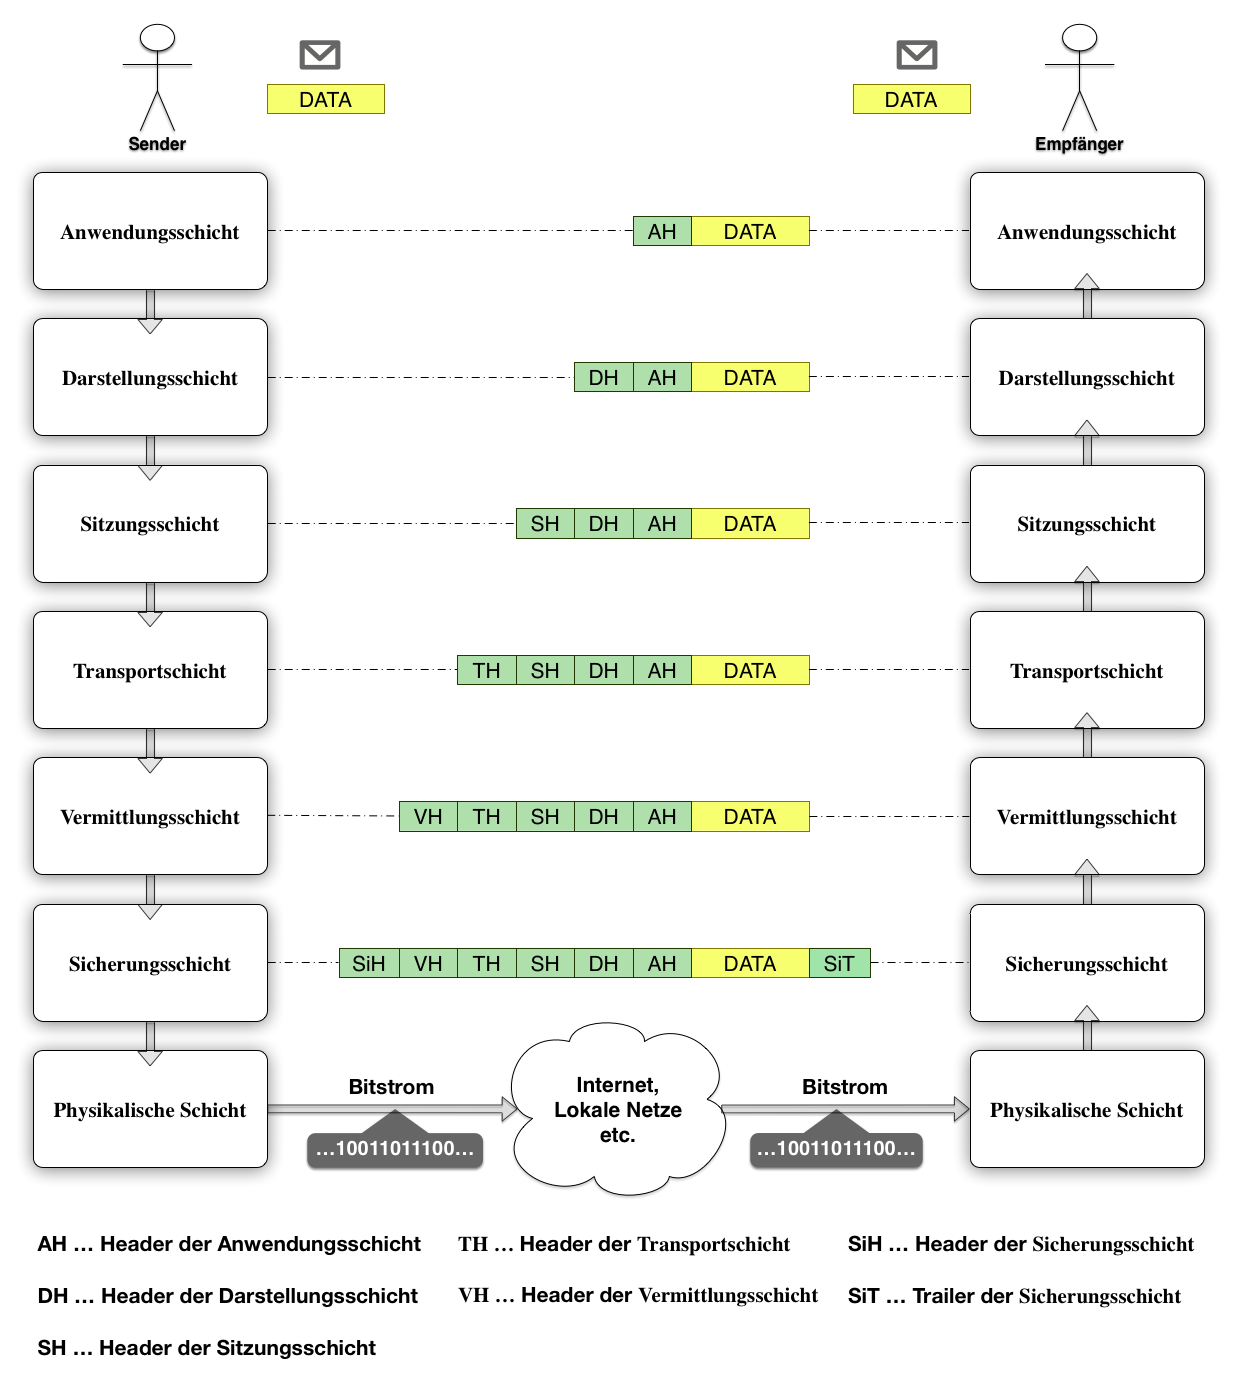
\includegraphics[width=400px,height=445px]{pictures/osi.png}
	}
	\caption[OSI-Schichtenmodell]{OSI-Schichtenmodell}\label{fig:osi}
\end{figure}

\paragraph{Sicherungsschicht (Data Link Layer)} Diese Schicht kann als \textbf{Datenverbindungsschicht} bezeichnet werden. Sie ist zuständig für eine zuverlässige Übertragung der Daten über die physische Verbindungen. Ihre Aufgaben sind
\begin{itemize}
	\item Logical Link Control (LLC)
	\item Media Access Control (MAC)
	\item Datengestaltung
	\item Adressierung
	\item Fehlererkennung und Fehlerbehebung
	\item Physikalische Layerstandardisierung
\end{itemize}
\textit{Beispiel}: Hardwareadressen, Ethernet, ARP etc.

\paragraph{Vermittlungsschicht (Network Layer)} Die Vermittlungsschicht hat die Aufgabe die \textbf{Verbindung aufzubauen}. Diese Schicht bestimmt, wie die Daten an das Empfängergerät gesendet werden sollen. Die Aufgaben sind
\begin{itemize}
	\item Logische Adressierung
	\item Routing
	\item Datagramm-Kapselung
	\item Fehlerbehandlung und Diagnose
\end{itemize}
\textit{Beispiel}: Quality of Service (QoS), Routing, IP-Protokoll, ICMP etc.

\paragraph{Transportschicht (Transport Layer)} Diese Schicht beschreibt die \textbf{Sicherungsmechanismen} für einen zuverlässigen Datentransport und garantiert die fehlerfreie Übertragung durch Fehlererkennungs- und Korrekturverfahren. Ihre wichtigsten Aufgaben sind
\begin{itemize}
	\item Adressierung auf der Prozess-Stufe
	\item Multiplexen und Demultiplexen
	\item Segmentierung, Verpackung, und Zusammenbau
	\item Verbindungsaufbau, Management, und Kündigung
	\item Anerkennung und Weiterleitung
	\item Flusskontrolle
\end{itemize}
\textit{Beispiel}: TCP- und UDP-Protokoll.

\paragraph{Sitzungsschicht (Session Layer)} Die Sitzungsschicht könnte als \textbf{Kommunikationssteuerschicht} bezeichnet werden. Sie beschäftigt sich mit der Verwaltung der Verbindungen zwischen den Anwendungen. Sie stellt ihre Werkzeugsätze bzw. die Befehlssätze als bidirektionale Kommunikation für höhere Protokolle, Anwendungsprogramme oder für die APIs zur Verfügung. Ihre bekanntesten Aufgaben sind
\begin{itemize}
	\item Datenflusssteuerung
	\item Dialogkontrolle und Koordination
	\item Datenzwischenspeicherung
\end{itemize}
\textit{Beispiel}: SMB-Protokoll, AppleTalk etc.

\paragraph{Darstellungsschicht (Presentation Layer)} Die Darstellungsschicht übernimmt die Daten von der Anwendungsschicht und wandelt sie in das Standardformat um (\textbf{Datenkonvertierungen}), um diese Daten für die darunterliegenden Schichten bereitzustellen. Ihre wichtigsten Aufgaben sind standardisierte
\begin{itemize}
	\item Übersetzungsverfahren
	\item Komprimierungsverfahren
	\item Kodierungsverfahren
\end{itemize}
\textit{Beispiel}: Standardisierung wie MPEG, TIFF, GIF und ASCII.

\paragraph{Anwendungsschicht (Application Layer)} Die Anwendungsschicht ist die oberste des OSI-Schichtenmodells. Sie bietet eine Schnittstelle für Benutzer oder für die Betriebssysteme, um Daten zu übertragen bzw. zu empfangen. \smallskip \smallskip

\textit{Beispiel}: Server-Client-Anwendungen, HTTP- und FTP-Client, Mail-Service, Kontroll- und User-Interfaces etc.

%%%%%%%%%%%%%%%%%%%%%%%%%%%%%%%%%%%%%%%%%%%%%%%%%%%%%%%%%%%%%%%%%%%%%%%%%%%%%%%
\subsection{TCP/IP-Schichtenmodell}

Das zweite wichtige Referenzmodell ist \textbf{TCP/IP-Schichtenmodell}, das auf Bedürfnisse der \textit{TCP/IP-Protokollfamilie} zugeschnitten ist. Anders als das OSI- ist das TCP/IP-Schichtenmodell nicht als Standard anerkannt. Dieses Modell wurde ab 1970 vom \textit{Department of Defense (DoD)} in den USA experimentiert. Später wurde das TCP/IP-Referenzmodell im Rahmen des \textit{ARPANET} entwickelt. Im Vergleich zu dem OSI-Schichtenmodell werden bei dem TCP/IP-Schichtenmodell nur vier übereinander liegende Schichten vorgesehen, wie in der \autoref{fig:tcpip} dargestellt wird. Jede Schicht hat mehrere Aufgaben und fügt einige zusätzliche Informationen als \textit{Header} in die gesendete Nachricht ein (\textbf{Einkapselung}). Einige Protokolle (z.B. Ethernet) fügen in der Netzzugangsschicht nicht nur einen Header, sondern auch einen \textit{Trailer} am Ende der gesendeten Nachricht hinzu. TCP/IP ist die heutige Netzwerkprotokollfamilie. \smallskip \smallskip

\begin{figure}[htbp]
	\centering
	\fbox{
		%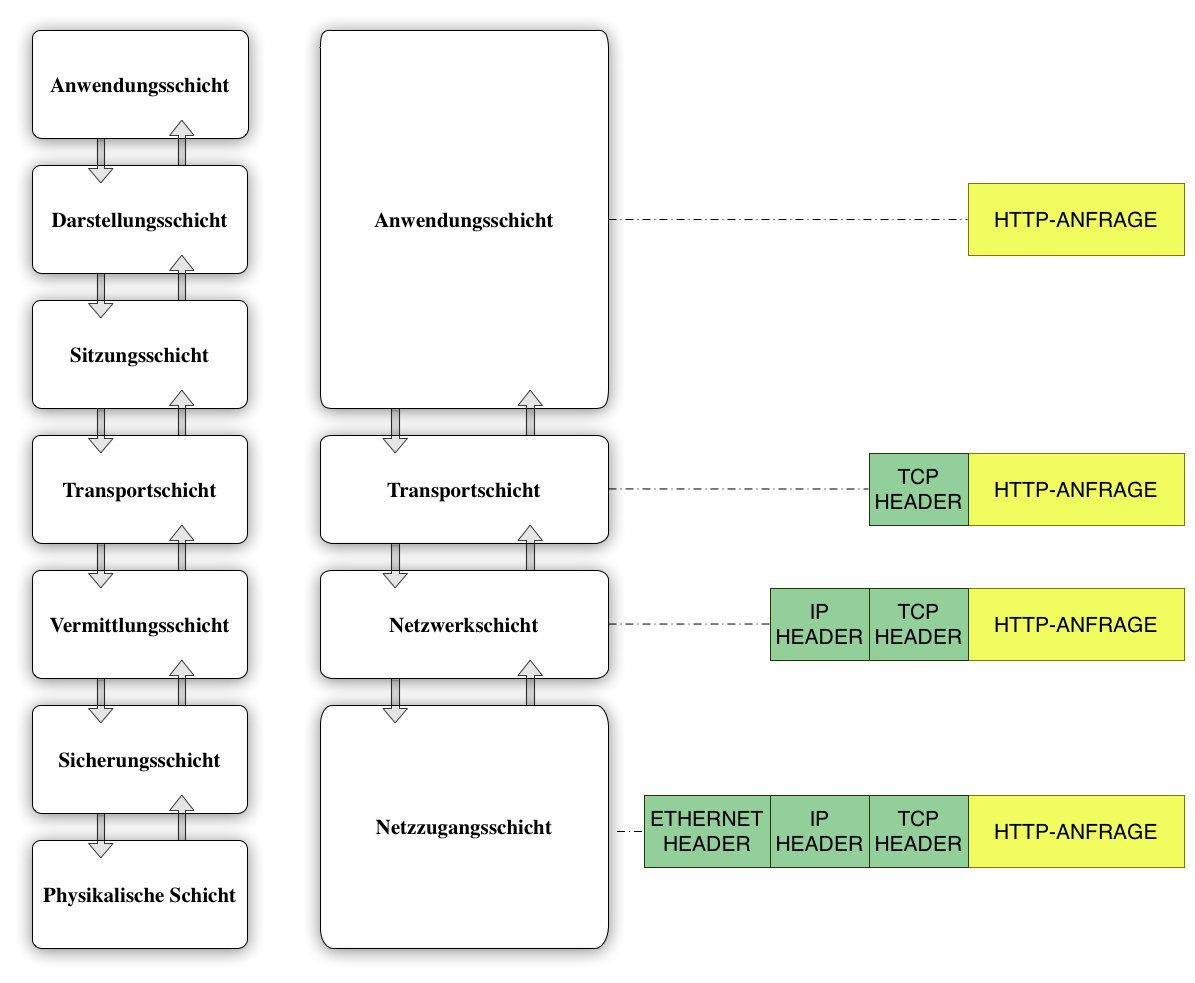
\includegraphics[width=400px,height=329px]{pictures/tcp_ip.png}
		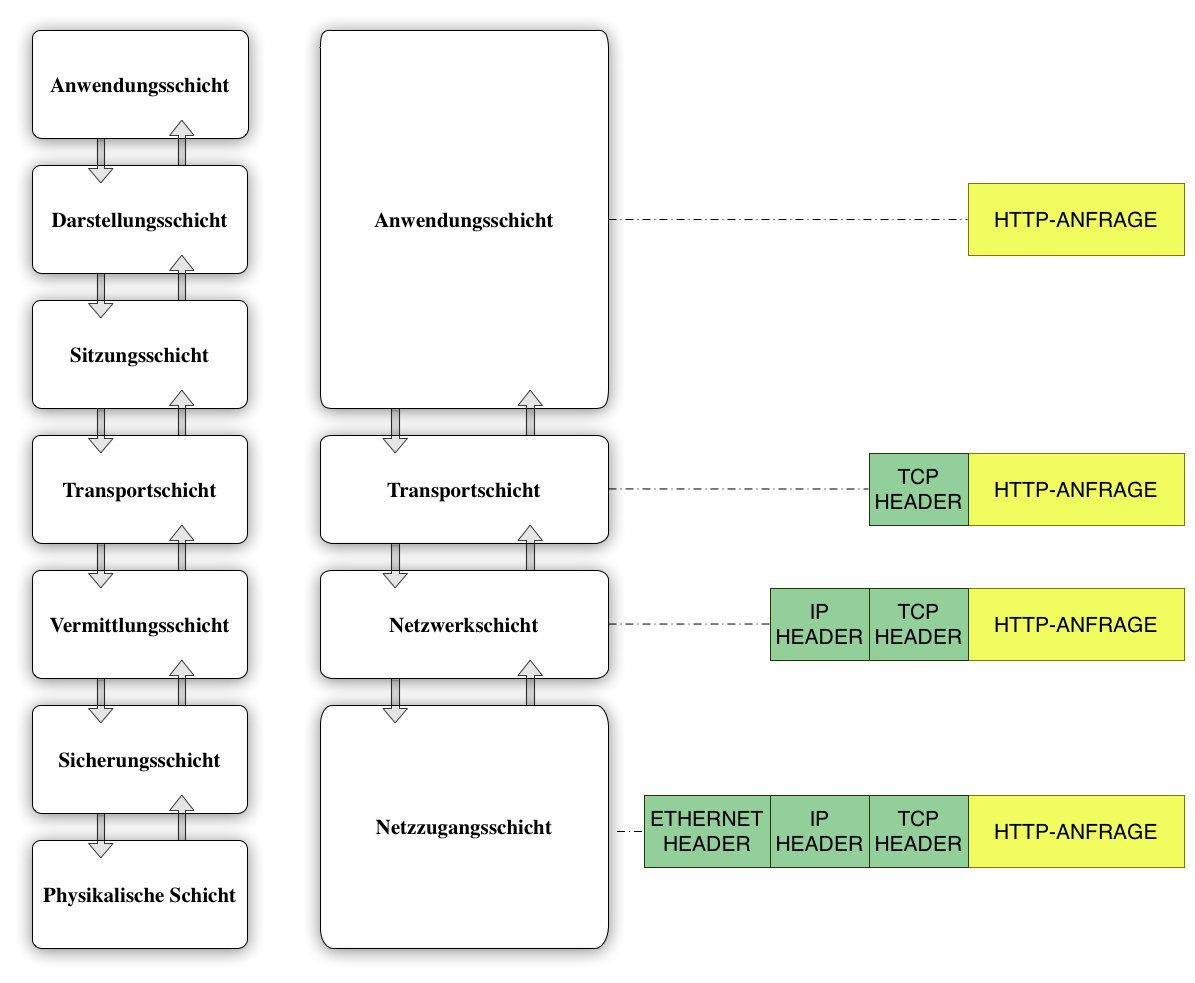
\includegraphics[width=330px,height=270px]{pictures/tcp_ip.png}
	}
	\caption[Vergleich zwischen OSI- und TCP/IP-Schichtenmodell]{Vergleich zwischen OSI- und TCP/IP-Schichtenmodell \cite{Jones:TCPIP} - durch Autor verändert.
	}\label{fig:tcpip}
\end{figure}

Das TCP/IP-Referenzmodell wird in der Literatur als ein 4-Schichtenmodell dargestellt. Andrew S. Tanenbaum hat in seinem Buch ''Computer Networks'' \cite{Tanenbaum:2010:CN:1942194} ein \textit{hybrides Referenzmodell} dargestellt, welches nicht als 4- sondern 5-Schichtenmodell präsentiert wird. In diesem Modell wird die Netzzugangsschicht in zwei Schichten aufgeteillt, die als \textit{Sicherungsschicht} und \textit{Bitübertragungsschicht} bezeichnet werden. \smallskip \smallskip

Die kurze Beschreibung jeder Schicht und dessen Aufgaben werden im Folgenden beschrieben. Die \autoref{fig:musterprotokolle} zeigt, wie beliebige Musterprotokolle in ihren jeweiligen Schichten definiert werden. \smallskip \smallskip

\paragraph{Netzzugangsschicht (Data Link Layer)} Diese Schicht ist die Zusammenlegung der Aufgaben der physikalischen Schicht und der Sicherungsschicht aus dem OSI-Schichtenmodell. Beide Schichten werden in der Netzzugangsschicht vereint. Sie beschäftigt sich mit den Eigenschaften der verschiedenen Übertragungsmedien. Weiters hat sie die Aufgaben von Zugriffsverfahren und zuverlässiger Übertragung der Nachricht über die Übertragungsmedien.

\paragraph{Netzwerkschicht (Network Layer)} Die Aufgaben der Netzwerksschicht sind Aufbau der Verbindung und die Weitervermittlung von Daten in einem logischen Netz. Dies bedeutet, dass das Internet-Protokoll für die Adressierung und Versendung der Datenpakete verantwortlich ist.

\begin{figure}[htbp]
	\centering
	\fbox{
		%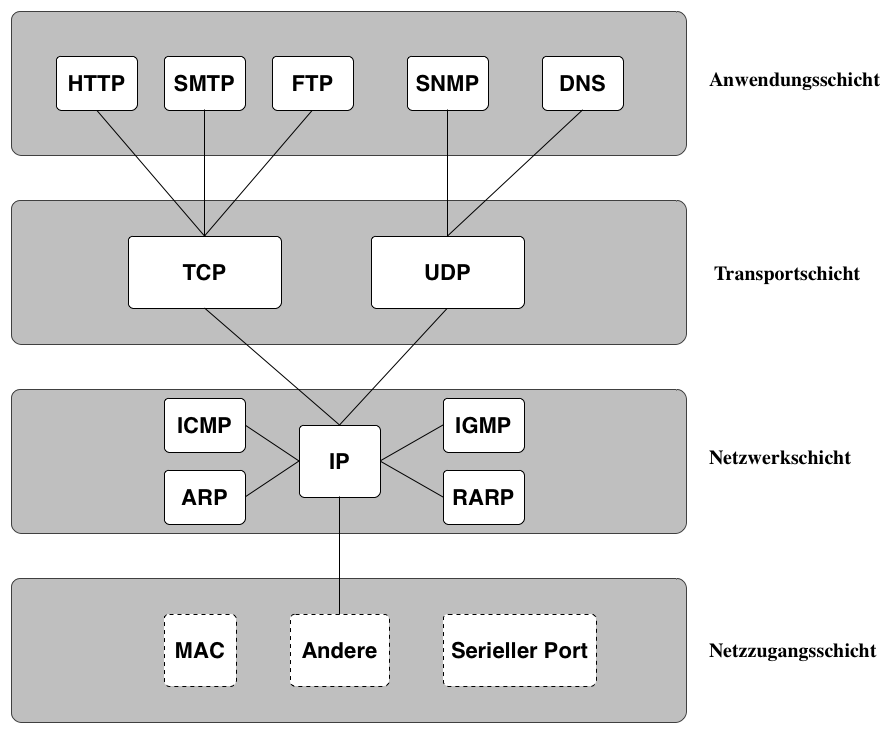
\includegraphics[width=350px,height=285px]{pictures/musterprotokolle.png}
		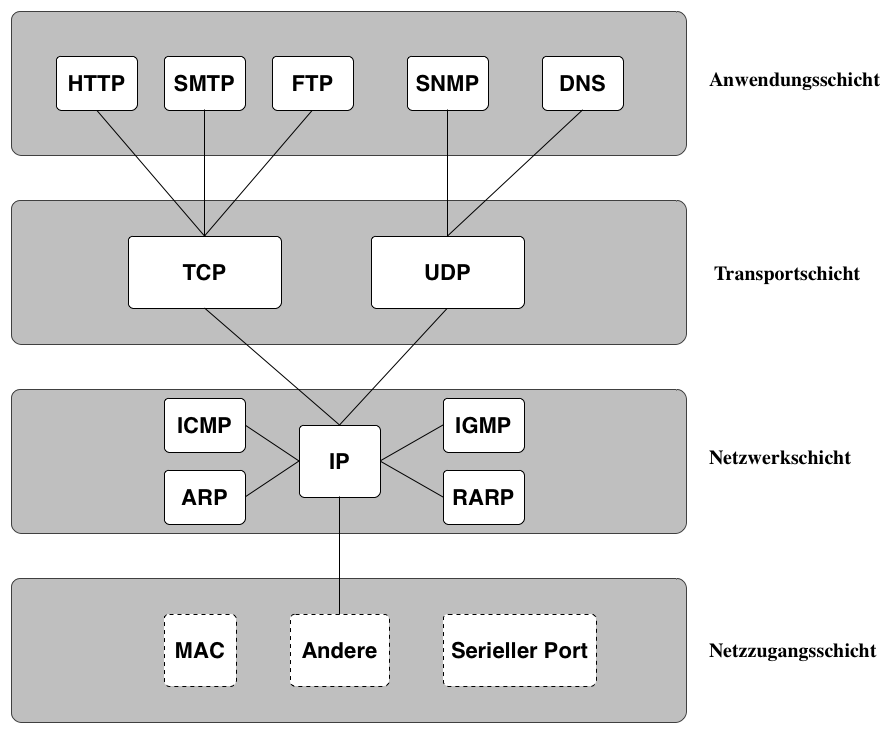
\includegraphics[width=245px,height=200px]{pictures/musterprotokolle.png}
	}
	\caption[Musterprotokolle in ihren jeweiligen Schichten]{Musterprotokolle in ihren jeweiligen Schichten \cite{Jones:TCPIP}}\label{fig:musterprotokolle} - durch Autor verändert.
\end{figure}

\paragraph{Transportschicht (Transport Layer)} Die Transportschicht besteht aus zwei Protokollen, nämlich TCP und UDP. TCP ist ein verbindungsloses Protokoll und stellt Host-zu-Host-Datendienste zur Verfügung. 

\paragraph{Anwendungsschicht (Application Layer)} Die Anwendungsschicht enthält alle möglichen Protokolle, welche von Anwendungsprogrammen, von Betriebssystemen oder von Prozessen um auf das Netzwerk zugreifen zu können, verwendet wird. 

%%%%%%%%%%%%%%%%%%%%%%%%%%%%%%%%%%%%%%%%%%%%%%%%%%%%%%%%%%%%%%%%%%%%%%%%%%%%%%%
\subsection{Internet-Protokolle}

Jede Schicht des OSI- bzw. des TCP/IP-Schichtenmodells hat die Aufgabe, interne Dienste für die benachbarten Schichten anzubieten. Diese Aufgaben sind durch Protokolle geregelt. Die \autoref{fig:internet-protokolle} zeigt an, welche Schicht aus welchen Protokollen besteht. \smallskip \smallskip

Wie schon angeschnitten wurde, findet die Übertragung über das Ethernet-Kanal statt, welches in der Netzzugangsschich liegt. In der darüber liegenden Schicht (Netzwerkschicht) ist das Internet-Protokoll für den Verbindungsaufbau, Adressierung und Vermittlung zwischen den kommunizierenden Hosts verantwortlich. Das ARP befindet sich auch in dieser Schicht. Außerdem ist hier auch das ICMP platziert, welches für Statusinformationen des Zielhosts mittels des Befehls \code{ping}\footnote{ist ein klassisches Werkzeug für die Verbindungsprüfung und wurde von Mike Muuss erst im Jahr 1983 in 4.3BSD entwickelt.} abfragt. \smallskip \smallskip

% internet protocol: http://tools.ietf.org/html/rfc791
\begin{figure}[htbp]
	\centering
%	\fbox{
		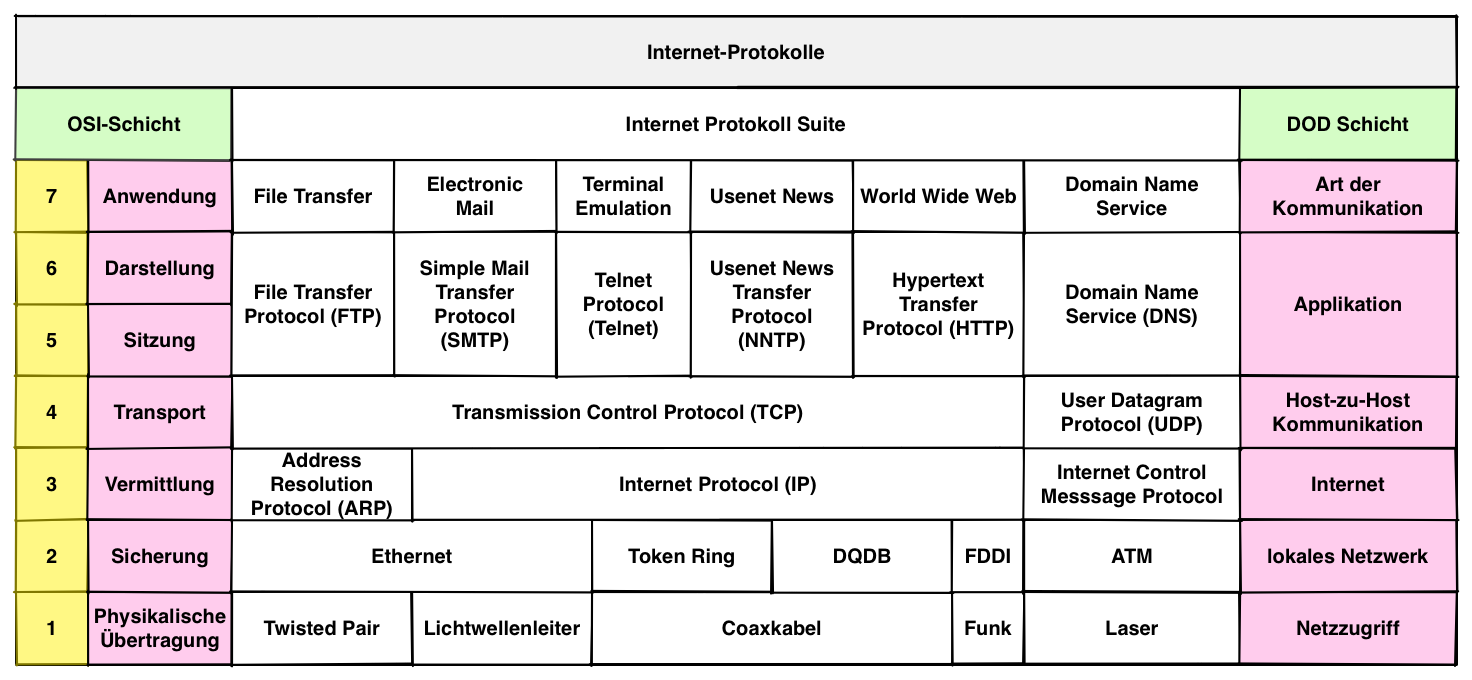
\includegraphics[width=450px,height=250px]{pictures/internet-protokolle.png}
%	}
	\caption[Internet-Protokolle]{Internet-Protokolle \cite{netzmafia}}\label{fig:internet-protokolle}
\end{figure}

Das TCP ist in der vierten OSI-Schicht und verantwortlich für einen zuverlässigen Datentransport. Nebenan ist das UDP für eine kurze Netzwerkmeldung zuständig, welches in dieser Arbeit realisiert wurde. 


%%%%%%%%%%%%%%%%%%%%%%%%%%%%%%%%%%%%%%%%%%%%%%%%%%%%%%%%%%%%%%%%%%%%%%%%%%%%%%%
\subsubsection{Ethernet}

Das Ethernet ist in den 1970er Jahren am \textit{Xerox Palo Alto Research Center} (PARC) entworfen worden. Die erste Version des Ethernets wurde ab 1980 vom IEEE in der Arbeitsgruppe 802 weiterentwickelt. Im Jahr 1982 wurde eine neue Version von Ethernet, nämlich \textbf{Ethernet-II}, herausgegeben, welche in diser Arbeit verwendet wird. Später wurde es durch IEEE 802.3 standardisiert und weiterentwickelt, um wieder zu TCP/IP kompatibel zu werden. In der \autoref{fig:Metcalfe:ethernet} wird der ursprüngliche Ethernet-Entwurf von Robert M. Metcalfe die Netzwerkverbindung als Äther definiert. \smallskip \smallskip

Unter dem Standard-Ethernet wurde die spezifizierte Datenübertragungsrate von maximal 10 MBit/s realisiert. Weiters wurde Fast-Ethernet bis zu 100 MBit/s sowie auch das Gigabit-Ethernet bis zu 1000 MBit/s weiterentwickelt. \smallskip \smallskip

\begin{figure}[htbp]
	\centering
%	\fbox{
		%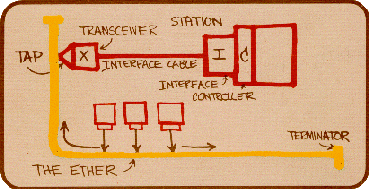
\includegraphics[width=320px,height=164px]{pictures/ethernet73.png}
		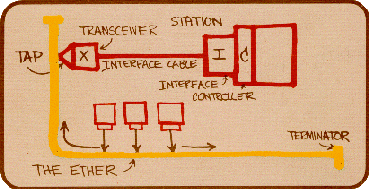
\includegraphics[width=250px,height=130px]{pictures/ethernet73.png}
%	}
	\caption[Ursprüngliche Ethernet-Entwurf von Robert M. Metcalfe]{ursprüngliche Ethernet-Entwurf von Robert M. Metcalfe \cite{IEEE:802.3}}\label{fig:Metcalfe:ethernet}
\end{figure}

Es wird in dem \autoref{sec:network} erwähnt, dass der ENC28J60-Mikrochip eine Schnittstelle vom Standart-Ethernet hat. Aus diesem Grund findet ein Standard-Ethernet in dieser Arbeit Verwendung. Es muss allerdings beachtet werden, dass ein Kabelsegment beim Standard-Ethernet eine Länge von 100 m nicht überschreiten darf. \smallskip \smallskip

\paragraph{Ethernet-II}\label{sub:ethernet-II}

Die gesendeten Daten bzw. Nachrichten werden immer mit Hilfe der Ethernet-Pakete transportiert. Die Ethernet-Pakete werden spezifisch als \textbf{frame} bezeichnet. Der Grundaufbau eines Ethernet-Frames ist bei allen Ethernet-Implementierungen identisch. Das \textbf{Typfeld} ist ein charakteristische Merkmal von Ethernet-II, das aus zwei Bytes im Anschluß an die Start- und Zieladressen besteht. Außerdem verfügt es über ein Kennzeichen, welches mittels eindeutiger zwei Byte-Zahl dargestellt wird, um das verwendete Protokoll bekanntzugeben. Es wird lediglich Ethernet-II-Frame in dieser Arbeit eingesetzt. Der Aufbau eines Ethernet-Datenpakets wird in der \autoref{fig:ethernet-II} dargestellt. 

\begin{figure}[htbp]
	\centering
%	\fbox{
		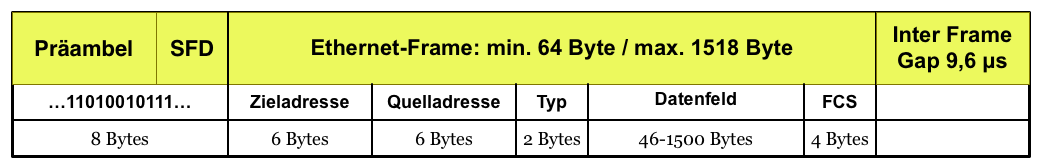
\includegraphics[width=450px,height=73px]{pictures/ethernet-II.png}
%	}
	\caption[Frame-Struktur von Ethernet-II]{Frame-Struktur von Ethernet-II \cite{netzmafia}}\label{fig:ethernet-II} - durch Autor verändert.
\end{figure}

Dem Ethernet-Frame wird eine \textbf{Präambel} vorangestellt. Sie besteht aus beliebigen Bit-Kombinatio-nen aus Nullen und Einsen in sieben Bytes, die für die Synchronisierung mit den Kommunikationspartnern benötigt werden. Der Präambel folgt \textbf{SFD} und dient als Rahmenbegrenzung. SFD führt eine eindeutige Bit-Kombination zur Signalisierung des Anfangs des Datenpakets. \smallskip \smallskip

Die \textbf{Ziel-} und \textbf{Quelladresse} besteht aus ihren MAC-Adressen von jeweils 6 Bytes. Für jede Netzwerkkarte gibt es eine eindeutige MAC-Adresse. \smallskip \smallskip

Das \textbf{Typfeld} dient als Kennzeichnung für den jeweiligen Protokolltyp. Es kann vorkommen, dass die Kennzeichnung keiner bekannten Type verweist. Genau in diesem Fall wird die Größe des Datenfeldes mittels dieser Zahl bekanntgegeben, da es keine Verpflichtung gibt, ein standardisiertes Protokoll zu verwenden. Einige Kennzeichen für zugehörige Protokolle sind in der folgenden \autoref{kennzeichen} beschrieben. Eine komplette öffentliche Liste befindet sich auf der Webseite von ''IANA'' \cite{Ethertypes}. 

\begin{table}[htbp]
	\centering
	\begin{tabular}{|c|c|}\hline
	   Kennzeichen & Protokoll \\ \hline \hline
	   0x0800 & IPv4 \\ \hline
	   0x0806 & ARP \\ \hline
	   0x8138 & Novell \\ \hline
	   0x86dd & IPv6 \\ \hline
	   0x809b & Appletalk \\ \hline
	 \end{tabular}
	 \caption{Kennzeichen für einige Protokolle}\label{kennzeichen}
\end{table}

Das \textbf{Datenfeld} besteht aus einigen Informationen, wie beispielsweise der TCP/IP-Header und beinhaltet gesendete Benutzerdaten. Die Länge des Datenfelds zum Datentransport beträgt zwischen 64 Bytes und 1518 Bytes. \smallskip \smallskip

Von der Zieladresse bis zum Ende des Datenfeldes wird ein \textbf{CRC} durchgeführt, die eine 32-Bit-Prüfsumme ist. Die Präambel und der SFD sind nicht in der Prüfsumme enthalten. Sie dient der Fehlererkennung durch die Anwendung eines speziellen Generatorpolynoms. Anschließend wird der CRC-Wert in das \textbf{FCS-Feld} des Ethernet-II-Frames gespeichert. Der Empfänger errechnet auch die Prüfsumme aus den empfangenen Daten und vergleicht diese mit den empfangenen FCS-Bytes. Nach dem Senden eines Frames erfolgt eine kurze Pause von 9,6 $\mu s$, die als \textbf{Inter Frame GAP} bezeichnet wird. 

%%%%%%%%%%%%%%%%%%%%%%%%%%%%%%%%%%%%%%%%%%%%%%%%%%%%%%%%%%%%%%%%%%%%%%%%%%%%%%%
\subsubsection{MAC-Adresse}\label{subsection:mac}

Jede Netzwerkkarte hat eine eindeutige \textbf{MAC-Adresse} und wird auch als \textit{physikalische Adresse} bezeichnet, beispielsweise ''00:23:32:cc:ff:1a''. Ihre Aufgabe ist, die miteinander kommunizierenden Hosts zu identifizieren. Die MAC-Adresse besteht aus einer Reihenfolge mit sechs Bytes (also 48 Bits\footnote{ermöglicht insgesamt $2^{48}$ MAC-Adressen.}) und wird mit dem hexadezimalen Zahlensystem dargestellt. In UNIX basierten Systemen erscheinen die MAC-Adresse der Netzwerkgeräte sowie Ethernet oder WiFi mit dem Befehl \code{ifconfig}\footnote{In manchen GNU/Linux-Systemen befindet sich kein Befehl \code{ifconfig}, sondern es gibt eigene Befehle sowie \code{ip} bzw. \code{netstat -ia} oder eigene vorhandene Systemdatei unter dem ''/etc''-Verzeichnis, in der die Netzwerkspezifikationen dargestellt werden.} und können manuell geändert werden. Das Format der MAC-Adresse ist in der \autoref{fig:mac_adress} zu sehen. \smallskip \smallskip

\begin{itemize}
	\item \textbf{I/G = 0:} Individual-Adresse (Unicast Address), das Ziel ist ein einzelnes Gerät bzw. ein Host
\end{itemize}

\begin{figure}[htbp]
	\centering
%	\fbox{
		%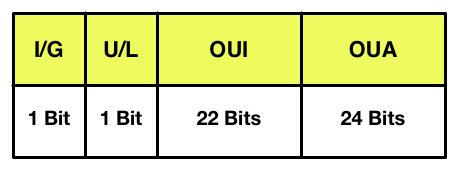
\includegraphics[width=250px,height=93px]{pictures/mac_adress.png}
		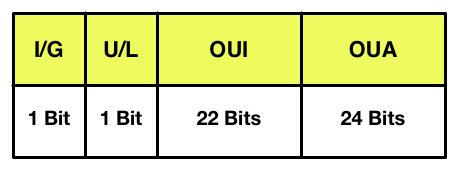
\includegraphics[width=190px,height=70px]{pictures/mac_adress.png}
%	}
	\caption[Format der MAC-Adress]{Format der MAC-Adress \cite{netzmafia}}\label{fig:mac_adress}
\end{figure}

\begin{itemize}
	\item \textbf{I/G = 1:} Gruppen-Adresse (Multicast Address), das Ziel ist eine Gruppe im LAN (Multicast- oder Broadcast-Adresse) 
	\item \textbf{U/L = 0:} universelle eindeutige und veränderbare Adresse bzw. MAC-Adresse
	\item \textbf{U/L = 1:} lokale veränderbare Adresse bzw. logische Adresse
	\item \textbf{OUI (Organizationally Unique Identifier):} Herstellererkennung, die von IEEE vergeben wird
	\item \textbf{OUA (Organizationally Unique Address):} Private Kennzeichnung, die vom Hersteller vergeben wird
\end{itemize}

%%%%%%%%%%%%%%%%%%%%%%%%%%%%%%%%%%%%%%%%%%%%%%%%%%%%%%%%%%%%%%%%%%%%%%%%%%%%%%%
\subsubsection{Adressierung}
Um die Daten zwischen zwei kommunizierenden Hosts zu übertragen, muss eine eindeutige Adresse indentifiziert werden, damit die gesendeten Daten an den richtigen Zielhost zugestellt wird. Aus diesem Grund hat jeder Rechner, der an einen TCP/IP-Netzwerk angeschlossen ist, eine bestimmte Adresse, nämlich eine \textbf{IP-Adresse}. \smallskip \smallskip

Die IP-Adressen bestehen aus einer 32 Bit langen Zahl und werden in Form von vier Dezimalzahlen geschrieben, jeweils zu 8 Bit gruppiert und durch einen Punkt (.) getrennt, beispielsweise ''128.130.40.232''. Daher können maximal $2^{32} = 4.294.967.296$ Adressen dargestellt werden. Ursprünglich wurden die IP-Adressen in drei Klassen, A, B und C, unterteilt. Jede Klasse besteht aus den Teilen von Netzadresse (Network Identifier) und Hostadresse (Host Identifier). Um die IP-Adresse in die Netzadresse und Hostadresse zu zerlegen, wird eine \textbf{Netzmask} verwendet. %Die Netzmask besteht immer aus einem \textbf{Präfix}- und einem \textbf{Suffix}-Teil. Je nach Netzwerkklasse wird die Länge der gesamten Adresse (32 Bit) nach Präfix und Suffix unterteilt.

\paragraph{Klasse A} In dieser Klasse gibt es 8 Bits, davon 1 Bit für Präfix und 7 freie Bit für Netzadresse. Die restlichen 24 Bit sind für die Hostadresse verwendbar. Das heißt, dass es sich in Klasse-A-Netzen maximal $2^7 = 128$ Netze und jeweils maximal $2^{24} = 16.777.216$ Hostadressen befinden können.

\paragraph{Klasse B} In der Klasse-B gibt es 16 Bits, davon 2 Bit für Präfix und 14 freie Bit für die Netzadresse. Die übrigen 16 Bit werden wieder für die Hostadresse verwendet. Es gibt maximal $2^{14} = 16.384$ Netzadresse mit jeweils höchstens $2^{16} = 65.536$ Hostadressen.

\paragraph{Klasse C} In Klasse-C-Netzen gibt es 24 Bit, davon 3 Bits für Präfix und 21 freie Bit für die Netzadresse. 8 Bits finden wie andere Klassen für die Hostadresse Verwendung. Es gibt maximal $2^{21} = 2.097.152$ Netzadressen mit jeweils höchstens $2^8 = 256$ Hostsadresse.

\begin{table}[htbp]
	\centering
	\begin{tabular}{|c|c|r|}\hline
	   Klasse & Präfix & Adressbereich \\ \hline \hline
	   A & 0 & 0.0.0.0 - 127.255.255.255 \\ \hline
	   B & 10 & 128.0.0.0 - 191.255.255.255 \\ \hline
	   C & 110 & 192.0.0.0 - 223.255.255.255 \\ \hline
	 \end{tabular}
	 \caption[Präfixe und Adressbereiche der Netzklassen]{Präfixe und Adressbereiche der Netzklassen \cite{Computernetze:kompakt}}
\end{table}

In der folgenden \autoref{klasse-c} ist ein Beispiel zur Klasse-C-Netzen mit der IP-Adresse 192.168.0.3 zu erkennen. Die UND-Verknüpfung der IP-Adresse mit der Netzmask ergibt die Netzadresse. Wiederum die UND-Verknüpfung zwischen der IP-Adresse und der invertierten Netzmask ergibt sich die Hostadresse. \smallskip \smallskip

\begin{table}[htbp]
	\centering
	\begin{tabular}{|c|c|c|c|c|c|}\hline
	   IP-Adresse 	& 192.168.0.3 	& 11000000 & 10101000 & 00000000 & 00000011 \\ \hline
	   Netzmask 	& 255.255.255.0 & 11111111 & 11111111 & 11111111 & 00000000 \\ \hline
	   inv. Netzmask 	& 0.0.0.255 & 00000000 & 00000000 & 00000000 & 11111111 \\ \hline
	   Netzadresse 	& 192.168.0.0 	& 11000000 & 10101000 & 00000000 & 00000000 \\ \hline
	   Hostadresse 	& 0.0.0.3		& 00000000 & 00000000 & 00000000 & 00000011 \\ \hline
	 \end{tabular}
	 \caption{Beispiel im Klasse-C}\label{klasse-c}
\end{table}

%%%%%%%%%%%%%%%%%%%%%%%%%%%%%%%%%%%%%%%%%%%%%%%%%%%%%%%%%%%%%%%%%%%%%%%%%%%%%%%
\subsubsection{ARP}

Wenn ein Datenpaket aus den oberen Schichten angekommen ist, muss es an die MAC-Adresse des Zielhosts adressiert werden. Das heißt, dass die MAC-Adresse des Zielhosts bekannt sein muss, damit die gesendeten Datenpakete beim Host zugestellt werden können. Aus diesem Grund hat ARP die Aufgabe, die IP-Adresse der Vermittlungsschicht in Hardware- und in MAC-Adressen der Sicherungsschicht umzusetzen. An dieser Stelle stellt ARP eine Tabelle, in der die logischen und physikalischen Adressen von lokalen Netzwerkgeräten gespeichert werden. Die ARP-Tabelle enthält drei Spalten, die aus IP-, MAC-Adresse und Typ bestehen. In UNIX basierten Systemen können die IP- und MAC-Adressen vom den beteiligten Rechnern im lokalen Netzwerk mit dem Befehl \code{arp -a} angezeigt werden. Die \autoref{fig:arp_protokoll} zeigt, welche Informationen das ARP-Protokoll beinhaltet. \smallskip \smallskip

Um die physikalischen Adressen der lokalen Rechnern zu ermitteln, wird eine ARP-Anforderung (ARP Request Broadcast) mit der Broadcast-Adresse von ''\textbf{FF:FF:FF:FF:FF:FF}'' gesendet. Danach aktualisiert jeder Empfänger seine Tabelle und sendet seine IP- und MAC-Adresse in die Quelladresse, welche in der Quell-Hardwareadresse der gesendeten ARP-Anforderung verfügbar ist, zurück. Diese Beantwortung der ARP-Anforderung heißt ARP Reply. \smallskip \smallskip

\begin{figure}[htbp]
	\centering
%	\fbox{
		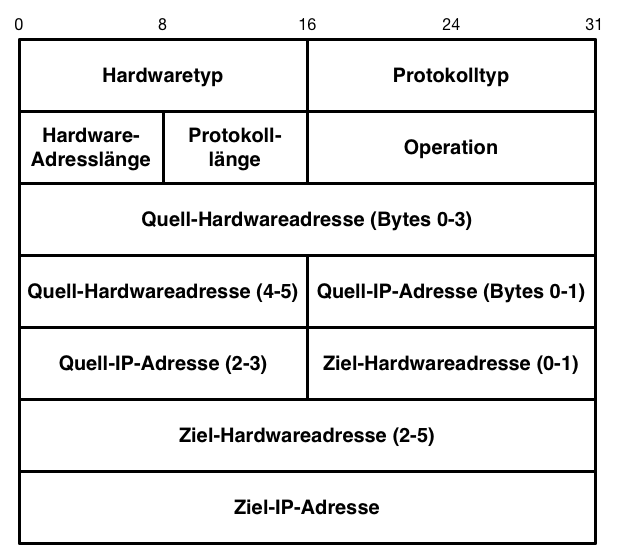
\includegraphics[width=235px,height=210px]{pictures/arp-protokoll.png}
		%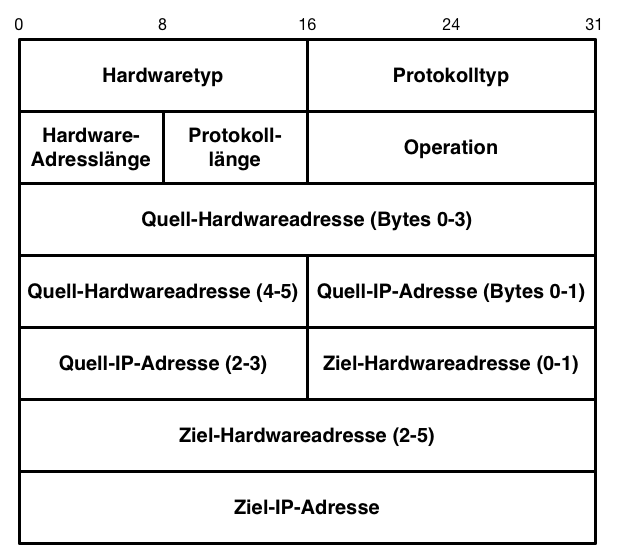
\includegraphics[width=200px,height=180px]{pictures/arp-protokoll.png}
%	}
	\caption[ARP-Protokoll]{ARP-Protokoll \cite{netzmafia}}\label{fig:arp_protokoll}
\end{figure}

%%%%%%%%%%%%%%%%%%%%%%%%%%%%%%%%%%%%%%%%%%%%%%%%%%%%%%%%%%%%%%%%%%%%%%%%%%%%%%%
\subsubsection{Internet Protokoll}

In der Vermittlungsschicht des OSI-Schichtenmodells und auch in der Netzwerkschicht des TCP/IP-Schichtenmodells befindet sich das Internet-Protokoll (kurz \textbf{IP}), um einen grundlegenden Netzdienst zur Verfügung zu stellen. IP hat auch ein eigenes Paketformat, das als \textbf{Datagramm} bezeichnet wird, bestehend aus dem Datenpaket und seinem eigenen Header. IP-Header ist der Bereich vom Anfangsbit bis zum Anfang des Datenbereichs. Die \autoref{fig:ip_protokoll} zeigt an, wie das Format von IP-Version-4 (IPv4) beschrieben wird. \smallskip \smallskip

\begin{figure}[htbp]
	\centering
%	\fbox{
		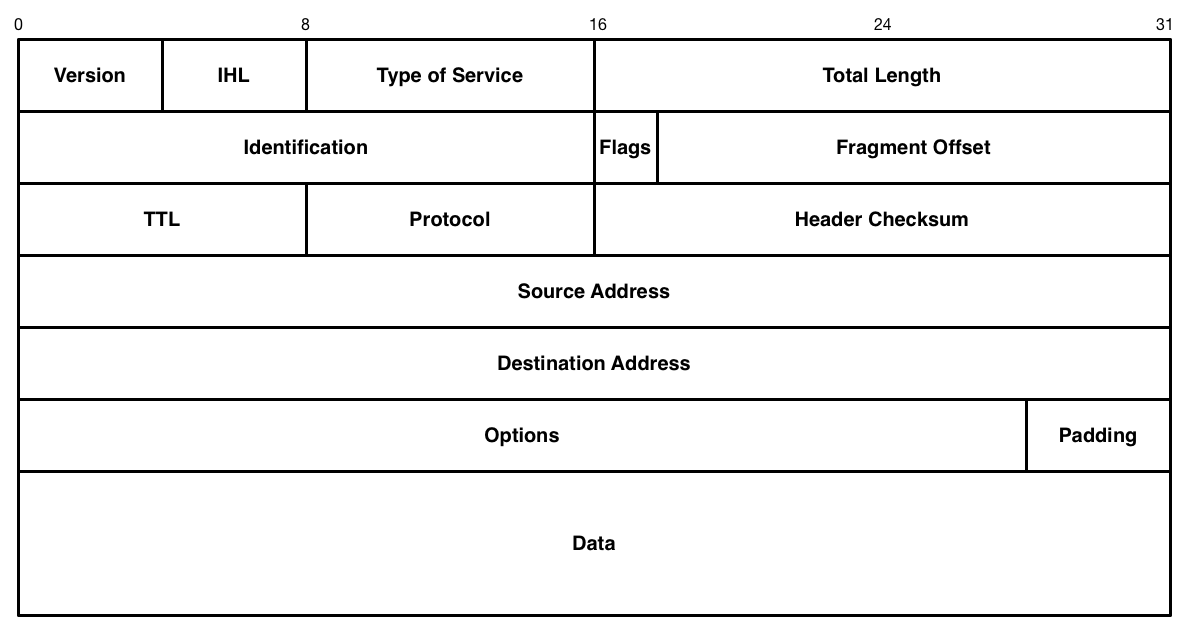
\includegraphics[width=450px,height=215px]{pictures/ip-protokoll.png}
		%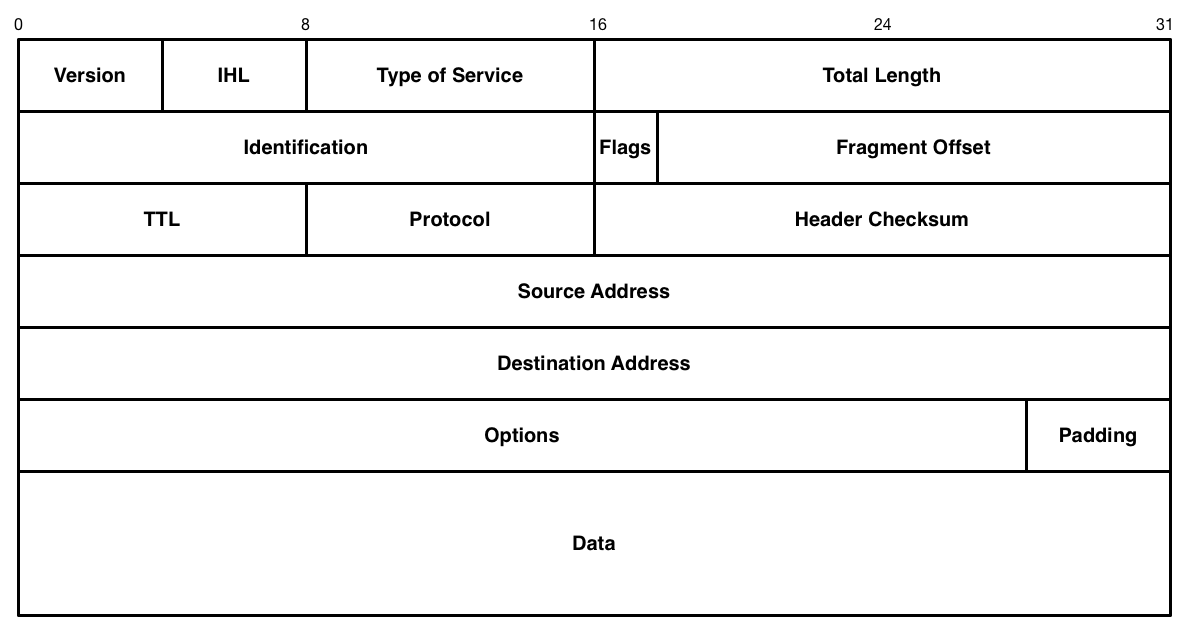
\includegraphics[width=400px,height=210px]{pictures/ip-protokoll.png}
%	}
	\caption[Internet Header Format]{Internet Header Format \cite{RFC:791}}\label{fig:ip_protokoll}
\end{figure}

Die Felder des Internet-Protokolls werden im Folgenden beschrieben:

\begin{itemize}
	\item \textbf{Version:} Kennzeichnung von verwendeten Internet-Protokoll-Version\footnote{Für IPv4 wird 4 verwendet.} (4 Bits)
	\item \textbf{IHL:} Länge des Internet-Protokoll-Headers (4 Bits)
	\item \textbf{Type of Service:} Steuerinformation sowie Priorisierung des Datagramms (8 Bits)\footnote{Dies Feld wurde in vergangenene Jahren unterschiedlich interpretiert. Es kann zwischen RFC-Nummern von 791, 2474 und 3168 verglichen werden.}
	\item \textbf{Total Length:} Länge des gesammten Datagramms (inkl. Kopfdaten, 16 Bits) ergibt eine maximale Länge von 64 KB\footnote{$2^{16}$ Bits = 64 KB.}
	\item \textbf{Identification:} Eindeutige Kennung eines Datagramms (16 Bits)
	\item \textbf{Flags:} Die Flags haben folgende Bedeutung:
		\begin{itemize}
			\item \textbf{Bit 0:} reserviert (immer $0$)
			\item \textbf{Bit 1:} DF (Don't Fragment), das Paket darf nicht fragmentiert werden, wenn das Bit logisch $1$ gesetzt ist
			\item \textbf{Bit 2:} MF (More Fragments), wenn er logisch $0$ ist, ist das Paket die letzte Fragmentierung
		\end{itemize}
	\item \textbf{Fragment Offset:} Anfangsadresse des fragmentierten Datagramms (13 Bits)
	\item \textbf{Time to Live:} Maximale Lebensdauer eines Datagramms (8 Bits)
	\item \textbf{Protocol:} Kennzeichnung des Protokolls (8 Bits)
	\item \textbf{Header Checksum:} Prüfsumme der Kopfdaten (16 Bits)
	\item \textbf{Source Address:} Internet-Adresse des Quellhosts des Datagramms (32 Bits)
	\item \textbf{Destination Address}: Internet-Adresse des Zielhosts des Datagramms (32 Bits)
	\item \textbf{Options:} Optionale Verwendung für weitere Informationen (24 Bits)
	\item \textbf{Padding:} Füllbits, damit unbenutzte Bytes mit Nullen ausgefüllt werden (8 Bits)
	\item \textbf{Data:} Beliebig gesendete bzw. empfangene Nachrichten
\end{itemize}

%%%%%%%%%%%%%%%%%%%%%%%%%%%%%%%%%%%%%%%%%%%%%%%%%%%%%%%%%%%%%%%%%%%%%%%%%%%%%%%
\subsubsection{ICMP}

Das Internet Control Message Protocol (ICMP) liegt beim Internet-Protokoll in der Vermittlungsschicht und ist ein Bestandteil des IP-Diagramms, wie in der \autoref{fig:icmp} dargestellt wird. Aus diesem Grund muss ICMP in IP-Pakete bzw. -Datagramme verpackt werden. Die Aufgabe von ICMP ist es, einen Bericht von Fehlermeldungen und Kontrollnachrichten über das Internet-Protokoll zu erstatten. \smallskip \smallskip

\begin{figure}[htbp]
	\centering
%	\fbox{
		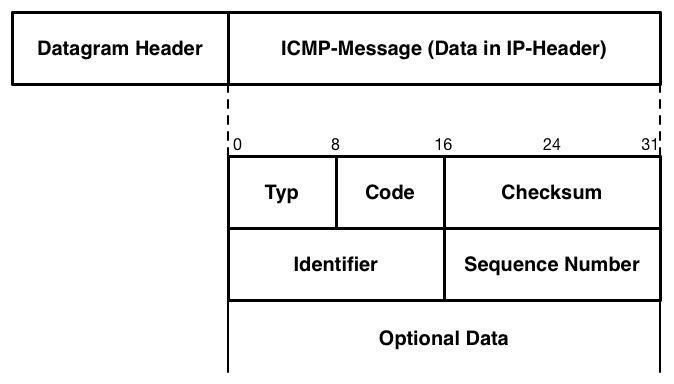
\includegraphics[width=260px,height=150px]{pictures/icmp.png}
		%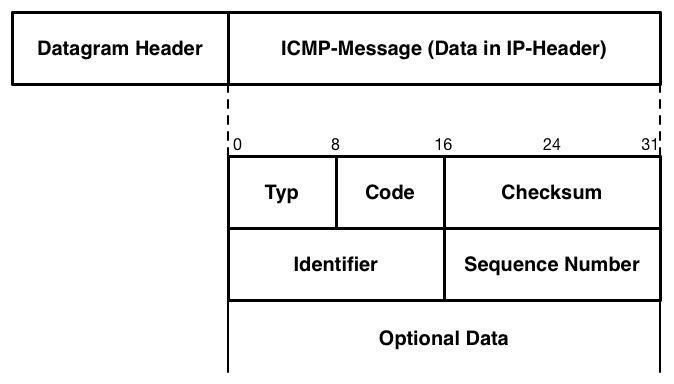
\includegraphics[width=200px,height=114px]{pictures/icmp.png}
%	}
	\caption[Internet Control Message Protocol]{ICMP-Header \cite{RFC:792}}\label{fig:icmp} - durch Autor verändert.
\end{figure}

Das Typ-Feld gibt an, zu welcher Klasse die ICMP-Nachricht gehört. Anbei spezifiziert das Code-Feld die Art der Nachricht. Checksum ist die Prüfsumme des kompletten Datagramms inklusive Header. Identifier ist ein Wert, um die Datagramme zuzuordnen. Die Sequenznummer unterscheidet die Datagramme. Die folgende \autoref{icmp} gibt eine genauere Beschreibung von Typ-Code-Kombinationen an. 

\begin{table}[htbp]
	\centering
	\begin{tabular}{|l|l|l|p{9cm}|}\hline
		Typ & Typname & Code & Bedeutung \\ \hline \hline
		0 & Echo-Antwort & 0 & Echo-Antwort (Anwort auf \code{ping}-Anfrage) \\ \hline
		3 & Ziel nicht erreichbar & 0 & Netzwerk nicht erreichbar \\

		\multirow{3}{*}{} 
			&  & 1 & Host nicht erreichbar \\
			&  & 2 & Protokoll nicht erreichbar \\ 
			&  & 3 & Port nicht erreichbar \\
	    	&  & 4 & Fragmentierung benötigt, aber nicht erlaubt (Don't Fragment gesetzt) \\
	    	&  & 5 & Source-Route fehlgeschlagen \\ 
	    	&  & 6 & Zielnetzwerk unbekannt \\
	    	&  & 7 & Ziel-Host unbekannt \tabularnewline \hline
%	    	&  & 8 & Quell-Host isoliert \\ 
%	    	&  & 9 & Kommunikation mit dem Zielnetzwerk ist verboten \\ 
%	    	&  & 10 & Kommunikation mit dem Zielhost ist verboten 
%	    	&  & 11 & Zielnetzwerk ist für den gegebenen Service-Typ nicht erreichbar \\ 
%	    	&  & 12 & Ziel-Host ist für den angegebenen Service-Typ nicht erreichbar \\ 
%	    	&  & 13 & Kommunikation verboten (durch Firewall) \\ \hline
		8 & \code{ping} (Echo-Anfrage) & 0 & Echo-Anfrage \\ \hline
		10 & Router Selection & 0 & (Router-Auswahl) \\ \hline
		11 & Zeitlimit überschritten & 0 & TTL (Time To Live) abgelaufen \\ \hline
	 	30 & Traceroute & 0 & Weg zum Ziel ermitteln \\ \hline
	\end{tabular}\caption[Typ-Code-Kombinationen von ICMP]{Typ-Code-Kombinationen von ICMP}\label{icmp}
\end{table}

%%%%%%%%%%%%%%%%%%%%%%%%%%%%%%%%%%%%%%%%%%%%%%%%%%%%%%%%%%%%%%%%%%%%%%%%%%%%%%%
\subsubsection{TCP}

Das Transmission Control Protocol (TCP) wird in der Transportsschicht des OSI-Schichtenmodells lokalisiert und bietet eine verbindungsorientierte, sichere Übertragung zwischen zwei kommunizierenden Hosts, im Prinzip eine Host-zu-Host-Verbindung. Die verbindungsorientierte Übertragung bedeutet, dass eine Kontrollfunktion während der Datenübertragung zwischen den Hosts ausgeführt wird, wodurch es sehr zuverlässig ist, weil die verlorengegangenen Daten erneut versendet werden können; das heißt, dass keine Daten verloren gehen. \smallskip \smallskip

Das TCP-Paket wird auch als \textbf{Segment} bezeichnet und enthält keine IP-Adresse, sondern Port-Nummer des Senders oder Empfängers, weil die IP-Adressen von kommunizierenden Hosts bereits im IP-Header angegeben werden (siehe \autoref{fig:ip_protokoll}). Daher findet die Kommunikation über Ports statt. Die folgende \autoref{fig:tcp} zeigt die Struktur eines Segments an. 

\begin{figure}[htbp]
	\centering
%	\fbox{
		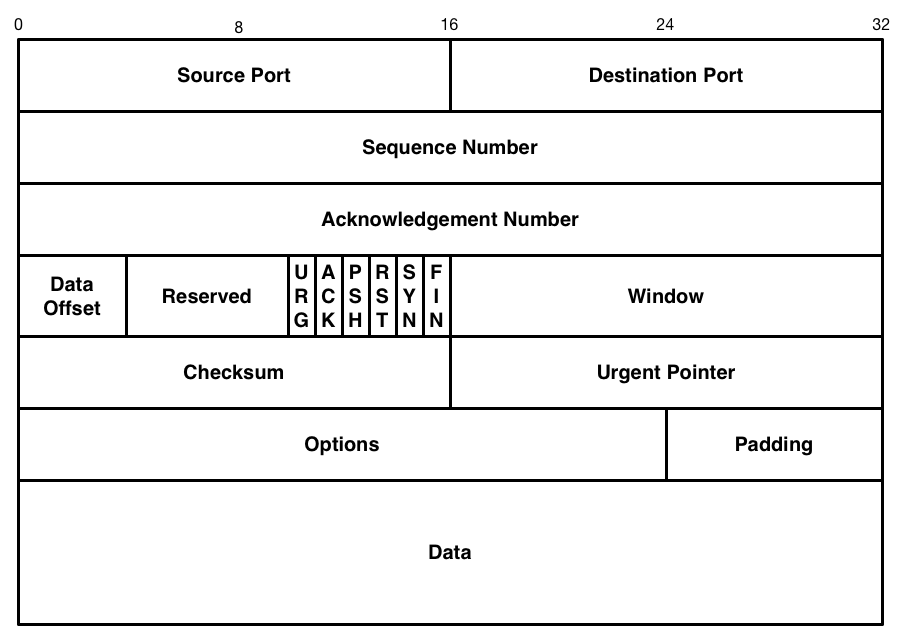
\includegraphics[width=356px,height=250px]{pictures/tcp.png}
		%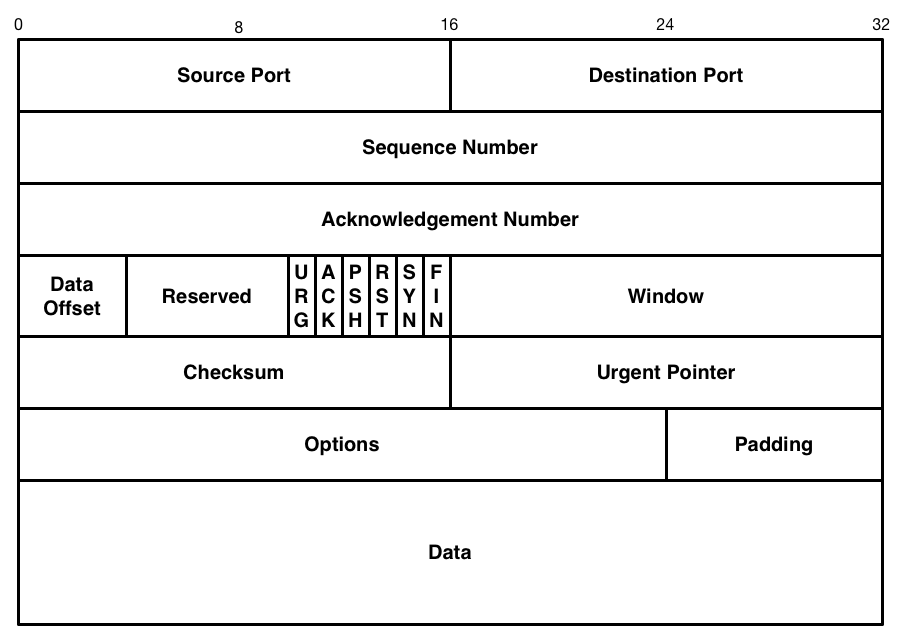
\includegraphics[width=300px,height=210px]{pictures/tcp.png}
%	}
	\caption[TCP Header Format]{TCP Header Format \cite{RFC:793}}\label{fig:tcp}
\end{figure}

Die Felder des TCP-Headers werden im Folgenden beschrieben:

\begin{itemize}
	\item \textbf{Source Port:} Die Portnummer des Senders besitzt eine Größe von 16 Bits und es stehen $2^{16} = 65536$ Ports zur Verfügung.
	\item \textbf{Destination Port:} Die Portnummer des Empfängers hat die Größe von 16 Bits und ermöglicht also 65536 Ports.
	\item \textbf{Sequence Number:} Die Nummer des aktuellen Segments innerhalb des Datenstromes.
	\item \textbf{Acknowledgement Number :} Die Sequenznummer des nächsten erwarteten Segments.
	\item \textbf{Data Offset:} Ist die Länge des Headers und enthält die Länge des TCP-Headers in 32-Bit Blöcken, damit der Empfänger weiß, wo die Nutzdaten im TCP-Segment anfangen.
	\item \textbf{Reserved:} Dieses Feld ist für zukünftige Entwicklungen reserviert und muss Null sein.
	\item \textbf{Control Bits:} Die folgenden sechs je 1 Bit große Felder werden für den Verbindungsaufbau, Datenaustausch und Verbindungsabbau benötigt. Jedes Bit erfüllt zwei unterschiedliche Funktionen, je nach dem ob es gesetzt ist oder nicht.
	\begin{itemize}
		\item \textbf{URG (Urgent):} Es wird gesetzt, wenn Urgent Pointer einen gültigen Wert enthält. 
		\item \textbf{ACK (Acknowledge):} ACK bestätigt die Gültigkeit der Bestätigungsnummer (ACK Number). 
		\item \textbf{PSH (Push):} PSH weist darauf hin, dass das Segment sofort in den Empfangspuffer übermittelt und direkt zur Anwendung gelangen kann.
		\item \textbf{RST (Reset):} Die Verbindung wird abgebrochen, wenn der Reset-Bit gesetzt ist.
		\item \textbf{SYN (Synchronize):} Der SYN-Bit ist gesetzt, während eine Verbindung aufgebaut wird. 
		\item \textbf{FIN (Finish):} Der Sender setzt das FIN-Bit, wenn die Übermittlung beendet ist.
	\end{itemize}
	\item \textbf{Window:} Das Window-Feld hat eine Anzahl der Bytes, die der Sender übermitteln darf, damit ein zuverlässiger Datentransport ohne Überlaufen des Empfangspuffers erledigt werden kann.
	\item \textbf{Checksum:} Die Prüfsumme des Datagramms (inkl. TCP-Header und Data) ist für die Fehlererkennung zuständig.
	\item \textbf{Urgent Pointer:} Wenn das URG-Bit des Control-Bits gesetzt ist, dann bekommt der Urgent-Pointer eine Bedeutung und wird interpretiert. Er gibt die Position des letzten Bytes der Urgent-Daten im Datenstrom an.
	\item \textbf{Options:} Das Option-Feld enthält Zusatzinformationen. TCP kennt drei Optionen, die NOP, End of Option List und die Festlegung der maximalen Segmentgröße.
	\item \textbf{Padding:} Padding wird verwendet, um den Anfang und das Ende des 32-Bit TCP-Headers sicherzustellen, wenn es nötig ist. Das Padding besteht aus Nullen.
	\item \textbf{Data:} Die Nutzdaten, welche für Anwendungen gedacht sind.
\end{itemize}

%%%%%%%%%%%%%%%%%%%%%%%%%%%%%%%%%%%%%%%%%%%%%%%%%%%%%%%%%%%%%%%%%%%%%%%%%%%%%%%
\subsubsection{UDP}

Das User Datagram Protocol (UDP) ist ein minimales Protokoll in der Transportschicht des OSI-Schichtenmodells. Im Gegensatz zu TCP ist UDP kein zuverlässiger, verbindungsloser Dienst, weil hier keine Flußkontrolle zur Verfügung gestellt wird. Es gibt keine Garantie, dass ein gesendetes Datanpaket an der Empfängerseite ankommt. Die versendeten Daten gehen auf gut Glück auf die Reise ins Netz. Der Vorteil bei UDP ist, dass die Größe des UDP-Segments ziemlich klein und die Geschwindigkeit des Datentransports sehr hoch sind. Aus diesem Grund wird in dieser Arbeit ein UDP-Datagramm verwendet, weil die abgefragete Information nur aus einer kommastelligen Zahl besteht. Der Aufbau eines UDP-Datagramms ist ganz einfach, wie in der folgenden \autoref{fig:udp} zu sehen ist. \smallskip \smallskip

\begin{figure}[htbp]
	\centering
%	\fbox{
		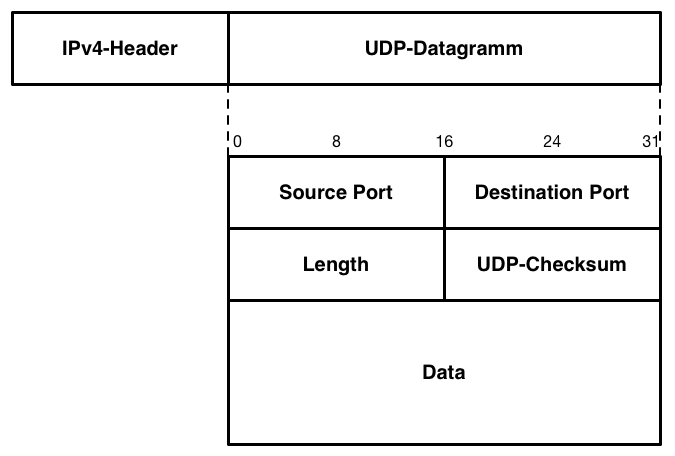
\includegraphics[width=300px,height=200px]{pictures/udp.png}
		%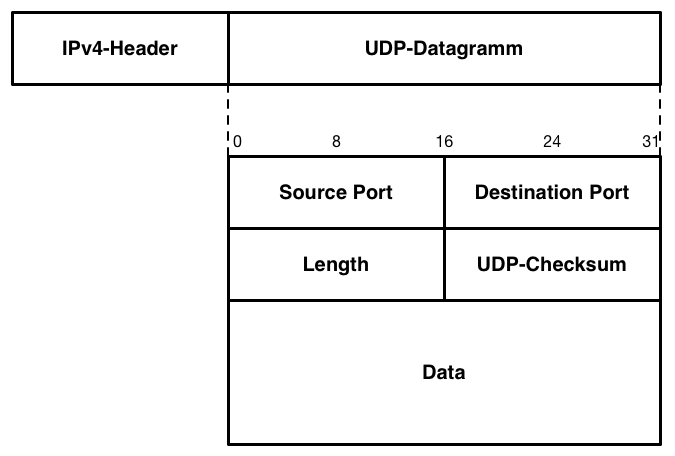
\includegraphics[width=200px,height=165px]{pictures/udp.png}
%	}
	\caption[User Datagram Protocol Header]{User Datagram Header Format \cite{Stevens:2009:TIP:1550778} - durch Autor verändert.
	}\label{fig:udp}
\end{figure}

Die Felder des UDP-Headers werden im Folgenden beschrieben:

\begin{itemize}
	\item \textbf{Source Port:} Die Portnummer des Senders, welche Werte von 0 bis 65536 annehmen kann.
	\item \textbf{Destination Port:} Die Portnummer des Empfänger.
	\item \textbf{Length:} Die Länge des UDP-Datagramms (inkl. UDP-Header).
	\item \textbf{Checksum:} Prüffsumme wird optional verwendet. Falls es nicht verwendet wird, wird der Inhalt mit Nullen dargestellt.
	\item \textbf{Data:} Benutzerdaten.
\end{itemize}

%%%%%%%%%%%%%%%%%%%%%%%%%%%%%%%%%%%%%%%%%%%%%%%%%%%%%%%%%%%%%%%%%%%%%%%%%%%%%%%
\subsection{RFC-Dokumente}

In der \autoref{rfcs} werden einige wichtigste und nützlichste RFC-Dokumente mit ihrer RFC-Nummer dargestellt. Für nützliche Informationen werden zwei unterschiedliche Webseiten angeboten: 

\begin{itemize}
	\item Die ganze Liste der RFC-Dokumente befinden sich auf der Webseite \textbf{rfc-editor} \cite{RFC-Editor}
	\item Häufig gestellte Fragen ist auf der Webseite \textbf{FAQs} \cite{FAQs} aufrufbar
\end{itemize} 

\begin{table}[htbp]
	\centering
	\begin{tabular}{|c|l|}\hline
	   RFC-Nummer & Beschreibung\\ \hline \hline
	   RFC 768 & User Datagram Protocol (UDP) \\ \hline
	   RFC 791 & Internet Protocol (IP) \\ \hline
	   RFC 792 & Internet Control Message Protocol (ICMP) \\ \hline
	   RFC 793 & Transmission Control Protocol (TCP) \\ \hline	   
	   RFC 821 & Simple Mail Transfer Protocol (SMTP) \\ \hline
	   RFC 826 & Ethernet Address Resolution Protocol (ARP) \\ \hline
	   RFC 854 & Telnet Protocol (Telnet) \\ \hline
	   RFC 959 & File Transfer Protocol (FTP) \\ \hline
	   RFC 977 & Usenet News Transfer Protocol (NNTP) \\ \hline
	   RFC 1034 & Domain Name Service (DNS) \\ \hline
	   RFC 1055 & Serial Line Internet Protocol (SLIP) \\ \hline
	   RFC 1533 & DHCP Options \\ \hline
	   RFC 1541 & Dynamic Host Configuration Protocol (DHCP) \\ \hline
%	   RFC 1866 & Hypertext Markup Language (HTML 2.0) \\ \hline
%	   RFC 2616 & Hypertext Transfer Protocol (HTTP 1.1) \\ \hline
	 \end{tabular}
	 \caption{RFC-Dokumente und ihre Beschreibungen}\label{rfcs}
\end{table}

%%%%%%%%%%%%%%%%%%%%%%%%%%%%%%%%%%%%%%%%%%%%%%%%%%%%%%%%%%%%%%%%%%%%%%%%%%%%%%%
\section{BSD-Sockets}

Der Aufbau eines Netzwerkens wurde im \autoref{chapter:protokoll} theoretisch beschrieben. Dieses Kapitel klärt auf, wie ein Netzwekaufbau mittels Betriebssystemfunktionen, sowie Socket-APIs erstellt werden kann. \smallskip \smallskip

Wie schon oben erwähnt wurde, muss ein Kanal zwischen kommunizierenden Hosts erstellt werden, wenn sie Nachrichten gegenseitig austauschen wollen. Dieser Kanal wird als \textbf{Socket}, sowie in UNIX-Systemen als \textbf{BSD-Socket}\footnote{wurde ertmal im Jahr 1983 für 4.2BSD auf der Berkeley Universität entwickelt.} bezeichnet. Die Socket-APIs liegen in der Sitzungsschicht des OSI-Schichtenmodells, sowie in der Anwendungsschicht des TCP/IP-Modells. Diese stellt eine Schnittstellt zwischen Anwendungsprogramme und der darunterliegenden Protokolle her.  Die \autoref{fig:tcp_udp} zeigt an, wie die Szenarien für TCP- und UDP-Verbindungen mittels BSD-APIs  sind. 

\subsection{Anlegen eines Sockets}

Beim Anlegen eines Sockets gibt es die \textbf{socket(2)}-Funktion, die im Erfolgsfall einen speziellen Datei- bzw. Socketdeskriptor zurückliefert, oder im Fehlerfall $-1$. Wenn die socket()-Funktion einen Socket erstellt, dann können die Nachrichten mit Hilfe des Socketdeskriptors ins Socket geschrieben oder aus dem Socket gelesen werden. 

\begin{minted}[linenos=false, frame=single, fontsize=\scriptsize]{c}
#include <sys/types.h>
#include <sys/socket.h>

int 
socket(int domain, int type, int protocol);
\end{minted} 
\smallskip \smallskip

\begin{figure}[htbp]
	\centering
	\fbox{
		%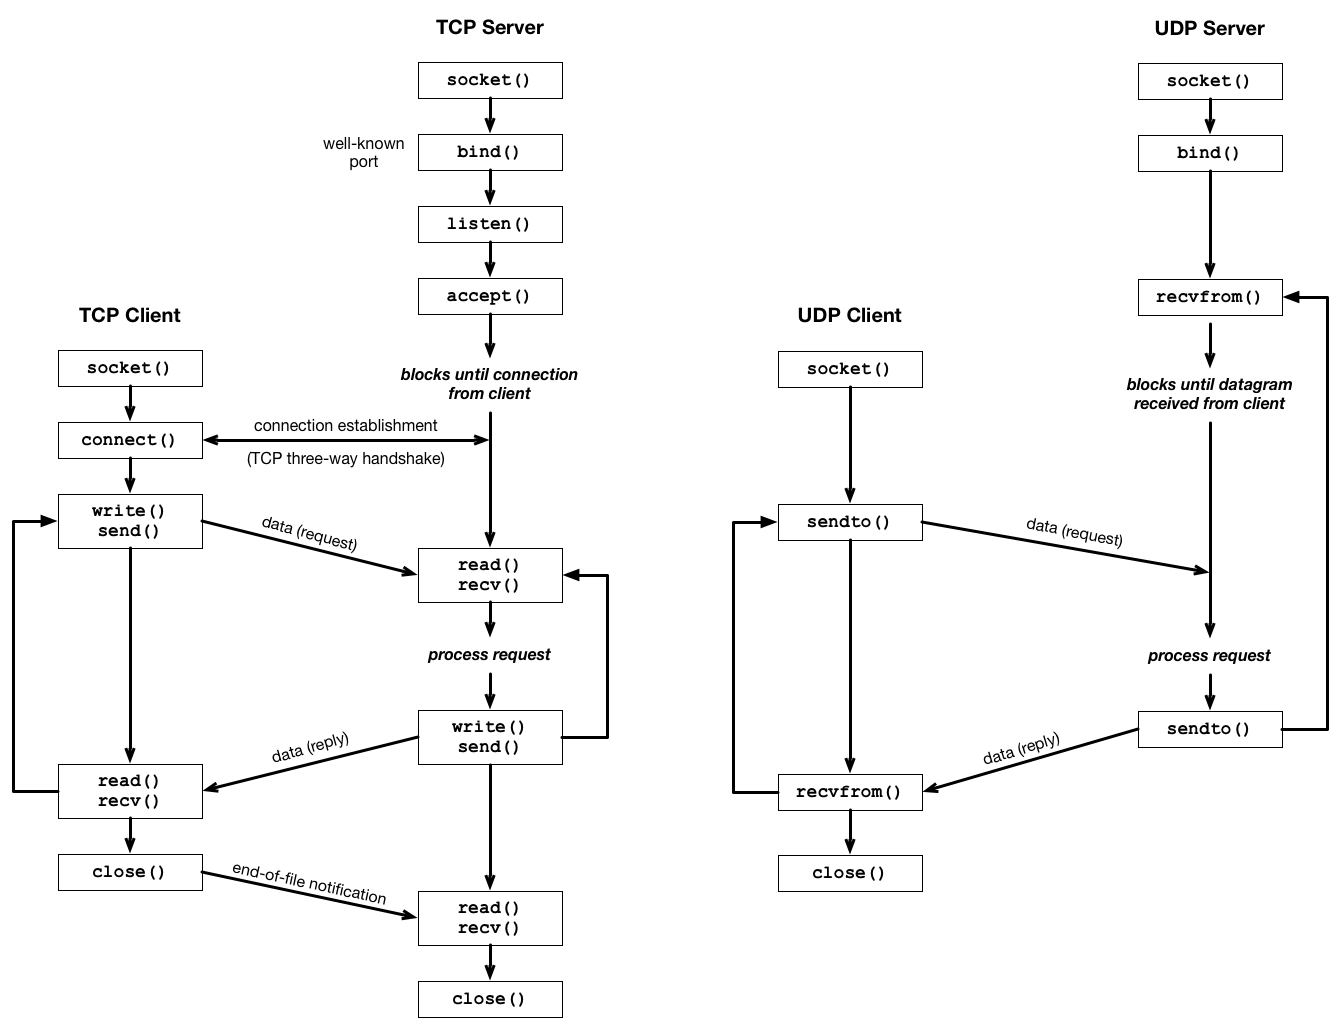
\includegraphics[width=400px,height=370px]{pictures/tcp_udp_szenarien.png}
		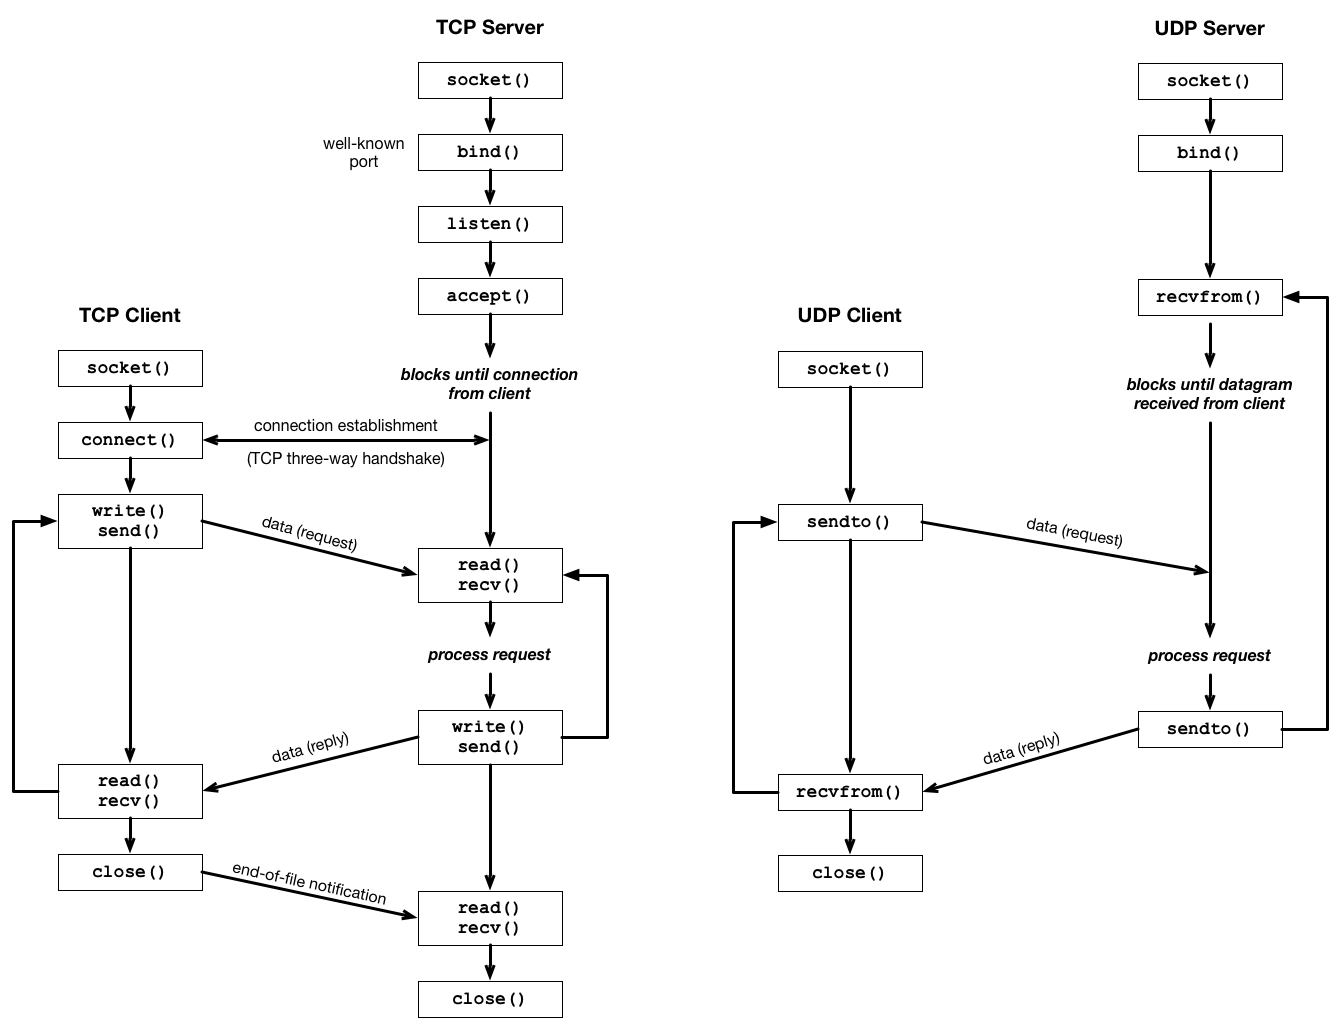
\includegraphics[width=450px,height=360px]{pictures/tcp_udp_szenarien.png}
	}
	\caption[Szenarien von TCP- und UDP-Kommunikationen]{Szenarien von TCP- und UDP-Kommunikationen \cite{Stevens:2004:UNP1}}\label{fig:tcp_udp} 
\end{figure}

Der Parameter \textit{domain} beschreibt die Art der Kommunikation sowie die gewünschte Adress- oder Protokollfamilie, mit der der neu angelegte Socket assoziiert wird. Diese Familien sind in der \textit{<sys/socket.h>} definiert, welche von POSIX.1 bekannt gegeben werden, wie einige Domains in der \autoref{socket:domain} beschrieben werden. \textbf{PF\_} steht hier für ''Protocol Family'' und \textbf{AF\_} für ''Address Family''. \textbf{PF\_} und \textbf{AF\_} haben dieselbe Konstante, weil sie aus historischen Gründen dieselben Implementierungen haben. \smallskip \smallskip

\begin{table}[htbp]
	\centering
	\begin{tabular}{|l|l|}\hline
	   Domain & Beschreibung \\ \hline \hline
	   AF\_INET & IPv4 Internet-Domain \\ \hline
	   AF\_UNIX & UNIX-Domain \\ \hline
	   PF\_LOCAL & Interne Host-Protokoll \\ \hline
	   AF\_UNSPEC & nicht spezifiert (unspecified) \\ \hline
	 \end{tabular}
	 \caption[Domäne der socket()-Funktion]{Domäne der socket()-Funktion}\label{socket:domain}
\end{table} \smallskip \smallskip

Der zweite Parameter der socket()-Funktion \textit{type} setzt das Sockettyp ein, um die Semantik der Kommunikation im Rahmen der zuvor definierten Domains zu bestimmen. Die von POSIX.1 definierten Sockettypen werden in der \autoref{socket:typ} dargestellt. \smallskip \smallskip

\begin{table}[htbp]
	\centering
	\begin{tabular}{|l|l|}\hline
	   Sockettyp & Beschreibung \\ \hline \hline
	   SOCK\_STREAM & Byte-Stream Socket \\ \hline
	   SOCK\_DGRAM & Datagram Socket \\ \hline
	   SOCK\_RAW & Raw Protocol Interface \\ \hline
	   SOCK\_SEQPACKET & Sequenced-Packet Socket \\ \hline
	 \end{tabular}
	 \caption[Soykettypen der socket()-Funktion]{Soykettypen der socket()-Funktion}\label{socket:typ}
\end{table} \smallskip \smallskip

Der letzte Parameter der socket()-Funktion \textit{protocol} bestimmt, welches Protokoll zwischen kommunizierenden Hosts eingestzt werden soll. Es wird oft \textit{NULL} gesetzt, um das Standardprotokoll für das angegebene Domain und Sockettyp zu verwenden. \smallskip \smallskip

Beispielsweise die Standardprotokolle: Es wird ein Sockettyp von SOCK\_STREAM und ein Domain von AF\_INET für ein Kommunikationsprotoll als TCP bestimmt. Oder es wird ein Sockettyp von SOCK\_DGRAM und ein Domain von AF\_INET für ein Kommunikationsprotokoll als UDP verwendet. Die verschiedenen definierten Möglichkeiten des \textit{protocol}-Parameters werden in der folgenden \autoref{socket:protocol} beschrieben. \smallskip \smallskip

\begin{table}[htbp]
	\centering
	\begin{tabular}{|l|l|}\hline
	   Protokoll & Beschreibung \\ \hline \hline
	   IPPROTO\_IP & IPv4 Internet-Protokoll \\ \hline
	   IPPROTO\_ICMP & Internet Control Message Protokoll \\ \hline
	   IPPROTO\_RAW & Raw IP-Pakete Protokoll \\ \hline
	   IPPROTO\_TCP &  Transmission Control Protokoll \\ \hline
	   IPPROTO\_UDP & User Datagram Protokoll \\ \hline
	 \end{tabular}
	 \caption[Protokolle der socket()-Funktion]{Protokolle der socket()-Funktion}\label{socket:protocol}
\end{table}

\subsection{Bindung eines Sockets}

Nach dem Anlegen eines Sockets wird es als \textit{unbenanntes Socket} bezeichnet, da es keine Protokoll-Adresse besitzt. Um die Nachrichten über einen Port mit Hilfe eines bestimmten Protokolls\footnote{Die einzigen von IANA bekanntegegebenen Portnummern für TCP und UDP mit den jeweiligen Beschreibungen werden in der Systemdatei ''/etc/services'' zugeordnet.} zu versenden, muss das Socket mit einer lokalen Protokoll-Adresse und Portnummer verbunden werden. Um die IP-Adresse und Portnummer an das Socket zuzuweisen, wird die \textbf{bind(2)}-Funktion verwendet. Wie die anderen Systemaufrufe, liefert die bind()-Funktion die Zahl $0$, wenn sie erfolgreich ist. Ansonsten wird im Fehlerfall $-1$ geliefert. \smallskip \smallskip

\begin{minted}[linenos=false, frame=single, fontsize=\scriptsize]{c}
#include <sys/types.h>
#include <sys/socket.h>

int
bind(int sockfd, const struct sockaddr *addr, socklen_t addrlen);
\end{minted}
\smallskip \smallskip

Der erste Parameter \textit{sockfd} ist der Socketdeskriptor, welcher mit der socket()-Funktion erzeugt wurde. Der zweite Parameter \textit{addr} ist ein Zeiger auf eine Socket-Adressstruktur \textit{struct sockaddr} (siehe \nameref{sec:datenstrukturen}). \textit{addrlen} ist die Länge der verwendeten Socket-Adressstruktur.

\subsection{Auflösung von Hostnamen}

Um die IP-Adresse von den Hostnamen aufzulösen, wird die \textbf{gethostbyname(3)}-Funktion verwendet. Sie bekommt einen Hostnamen und liefert einen Zeiger auf die Struktur \textit{hostent} zurück, welche die IP-Adresse und einige Informationen beinhaltet, wie im \nameref{sec:datenstrukturen} näher beschrieben wird. \smallskip \smallskip

\begin{minted}[linenos=false, frame=single, fontsize=\scriptsize]{c}
#include <netdb.h>

struct 
hostent *gethostbyname(const char *name);
\end{minted}

\subsection{Verbindungsaufbau}

Bis jetzt wurde ein Socket erstellt und mit der lokalen Protokoll-Adresse und Portnummer verbunden. Nun wird die Kommunikation zweiseitig, also erfolgt die Server- und die Client-Seite getrennt. 

\subsubsection{Verbindunganforderung}

Um eine Verbindungsanforderung aus der Client-Seite zu senden, steht \textbf{connect(2)}-Funktion zur Verfügung. Sie liefert im Erfolgsfall eine $0$, im Fehlerfall eine $-1$. \smallskip \smallskip

\begin{minted}[linenos=false, frame=single, fontsize=\scriptsize]{c}
#include <sys/types.h>
#include <sys/socket.h>

int
connect(int sockfd, const struct sockaddr *addr, socklen_t len);
\end{minted}
\smallskip \smallskip

Der erste Parameter ist \textit{sockfd}, der mittels \textit{socket()}-Funktion erzeugt wurde. Der zweite Parameter ist ein Zeiger auf der \textit{sockaddr}-Struktur, in der sich die Adresse des Servers befindet. \textit{len} ist die Länge der Struktur, die übergeben wird.

\subsubsection{Horchen}

Auf der Server-Seite wird eine am erzeugten Socket einkommende Verbindunganforderung mit der \textbf{listen(2)}-Funktion abgehorcht. Im Erfolgsfall liefert die listen()-Funktion den Wert $0$, ansonsten $-1$. \smallskip \smallskip

\begin{minted}[linenos=false, frame=single, fontsize=\scriptsize]{c}
#include <sys/types.h>
#include <sys/socket.h>

int
listen(int sockfd, int backlog);
\end{minted}
\smallskip \smallskip

Das erste Argument ist das horchende Socket, und das zweite bietet einen Hinweis auf die Anzahl der Verbindungsanforderungen. Dafür bildet das Betriebssystem eine Warteschlange. In der Header-Datei \textit{<sys/socket.h>} wurde \textit{SOMAXCONN} für die maximale Warteschlange als 128 vordefiniert. 

\subsubsection{Verbindungsannahme}

Nachdem eine Verbindungsanforderung an das erzeugte Socket mit der voreingestellten Portnummer angekommen ist, muss an der Server-Seite eine Akzeptierung dieser Anforderung mit Hilfe der \textbf{accept(2)}-Funktion angenommen werden. Diese Funktion nimmt eine Verbindungsanforderung aus der Warteschlange der listen()-Funktion, dann wird ein neues Socket mit dem gleichen Sockettyp, dem gleichen Protokoll und der gleichen Adressfamilie erstellt. Anschließend legt sie den neuen Socketdeskriptor für das neue Socket an. \smallskip \smallskip

\begin{minted}[linenos=false, frame=single, fontsize=\scriptsize]{c}
#include <sys/types.h>
#include <sys/socket.h>

int
accept(int sockfd, struct sockaddr *restrict addr, 
       socklen_t *restrict addrlen);
\end{minted}
\smallskip \smallskip

Das erste Argument ist der Socketdeskriptor aus der Warteschlange der listen()-Funktion. Der zweite Parameter ist der Zeiger auf eine \textit{sockaddr}-Struktur, in der die Socket-Informationen von \textit{sockfd}-Deskriptor für das neu angelegte Socket kopiert werden. \textit{addrlen} ist die Länge der kopierten Socket-Information. Im Erfolgsfall liefert die accept()-Funktion den Socketdeskriptor des akzeptierten Sockets, ansonsten $-1$.

\subsection{Datenübertragung}

Wenn eine Verbindung zwischen dem Server und dem Client aufgebaut wurde, dann erfolgt die Datenübertragung bzw. Nachrichtenaustausch zwischen kommunizierenden Hosts. 

\subsubsection{Datensendung}\label{sub:datensendung}

Um die Daten zu versenden, stehten drei Systemaufrufe zur Verfügung, also \textbf{send(2)}, \textbf{sendto(2)} und \textbf{sendmsg(2)}. Die \textit{send()}-Funktion darf nur verwendet werden, wenn das Socket in einem verbundenen Zustand ist. Jedoch die \textit{sendto()}- und \textit{sendmsg()}-Funktionen können jeder Zeit eine Nachricht versenden. Aus diesem Grund werden die \textit{sendto()}- und \textit{sendmsg()}-Funktionen üblicherweise für UDP-Sockets eingesetzt. Am Ende liefern diese drei Systemaufrufe die Anzahl der erfolgreich gesendeten Bytes, oder $-1$ im Fehlerfall. \smallskip \smallskip

\begin{minted}[linenos=false, frame=single, fontsize=\scriptsize]{c}
#include <sys/types.h>
#include <sys/socket.h>

ssize_t
send(int sockfd, const void *buf, size_t nbytes, int flags);

ssize_t
sendto(int sockfd, const void *buf, size_t nbytes, int flags,
       const struct sockaddr *destaddr, socklen_t destlen);

ssize_t
sendmsg(int sockfd, const struct msghdr *msg, int flags);
\end{minted}
\smallskip \smallskip

Der erste Parameter der \textit{send()}-Funktion ist der Socketdeskriptor, über den die Nachricht versendet wird. \textit{buf} ist ein Zeiger auf einen Puffer, der die zu versendenden Daten enthält. Die Länge dieser Daten wird mit \textit{len} angegeben. \textit{flags}\footnote{werden in der Header-Datei ''<sys/socket.h>'' definiert.} spezifiziert die Art der Datenübertragung, wie im folgenden Code-Feld beschrieben wird. \smallskip \smallskip

\begin{minted}[linenos=false, frame=single, fontsize=\scriptsize]{c}
#define MSG_OOB         0x1
#define MSG_PEEK        0x2  
#define MSG_DONTROUTE   0x4  
#define MSG_EOR         0x8 
... 
#define MSG_WAITALL     0x40 
...
#define MSG_EOF         0x100 
...
...
\end{minted}
\smallskip \smallskip

Die ersten vier Parameter der \textit{sendto()}-Funktion sind gleich wie die Parameter der \textit{send()}-Funktion. Der fünfte Parameter \textit{destaddr} ist der Zeiger auf die Zieladresse des Datagramms, während \textit{destlen} die Länge der Struktur der Zieladresse festlegt. \smallskip \smallskip

Die \textit{sendmsg()}-Funktion sendet eine spezifische Nachrichtenstruktur mit den oben beschriebenen Flag-Codes über \textit{flags} an den Socketdeskriptor \textit{sockfd}. Die Datenstruktur \textit{msghdr} wird im folgenden Code-Feld dargestellt. \smallskip \smallskip

\begin{minted}[linenos=false, frame=single, fontsize=\scriptsize]{c}
struct msghdr {
  void         *msg_name;       /* optinale Adresse                  */
  socklen_t     msg_namelen;    /* Laenge der Adresse                */
  struct iovec *msg_iov;        /* Datenfeld von Ein-/Ausgang-Puffer */
  int           msg_iovlen;     /* Anzahl der Elementen im Datenfeld */
  void         *msg_control;    /* nebenbetriebene Data              */
  socklen_t     msg_controllen; /* Anzahl von Data                   */
  int           msg_flags;      /* Flags fuer Empfangsdaten          */
};
\end{minted}

\subsubsection{Datenempfang}

Um die ankommenden Daten von einem verbundenen Socket einzulesen, stehen drei Systemaufrufe zur Verfügung, nämlich \textbf{recv(2)}, \textbf{recvfrom(2)} und \textbf{recvmsg(2)}. Die \textit{recv()}-Funktion arbeitet nur mit den verbundenen Sockets, jedoch die \textit{recvfrom()}- und \textit{recvmsg()}-Funktionen sind für nicht-verbundene Sockets geeignet. Die drei Funktionen liefern eine Anzahl der erfolgreich eingelesenen Bytes, ansonsten $-1$ im Fehlerfall. \smallskip \smallskip

\begin{minted}[linenos=false, frame=single, fontsize=\scriptsize]{c}
#include <sys/types.h>
#include <sys/socket.h>

ssize_t
recv(int sockfd, void *buf, size_t nbytes, int flags);

ssize_t
recvfrom(int sockfd, void *buf, size_t len, int flags,
         struct sockaddr *restrict addr, socklen_t *restrict addrlen);

ssize_t
recvmsg(int sockfd, struct msghdr *msg, int flags);
\end{minted}
%\smallskip \smallskip

Die \textit{recv()}-Funktion liest mit der gegebenen Länge von Bytes \textit{nbytes} aus dem Socketdeskriptor \textit{sockfd} ein und speichert sie in den Puffer \textit{buf}. Der Parameter \textit{flags} spezifiziert die Art der Datenübertragung, wie im obigen Code-Feld beschrieben wurde. \smallskip \smallskip

Die ersten vier Parameter der \textit{recvfrom()}-Funktion sind gleich wie die \textit{recv()}-Funktion. Der Parameter \textit{addr} enthält die Quelladresse des Datagramms, während \textit{addrlen} die Länge der Struktur darstellt. \smallskip \smallskip

Die \textit{recvmsg()}-Funktion empfängt eine spezifische Nachrichtenstruktur mit den oben beschriebenen Flag-Codes \textit{flags} aus dem Socketdeskriptor \textit{sockfd}. Die Datenstruktur \textit{msghdr} wurde oben beschrieben.

\subsection{Abschluss der Kommunikation}

Wenn die Datenübertragung erfolgreich ist, dann sollten die geöffnete Sockets geschlossen werden. In diesem Erfolgsfall wird die \textbf{close(2)}-Funktion verwendet, um den File- bzw. Socketdesckriptor zu löschen. Um ihn zu entfernen, wird dafür der Parameter \textit{fildes} verwendet. Im Erfolgsfall liefert die \textit{close()}-Funktion eine $0$ zurück, ansonsten $-1$ im Fehlerfall. \smallskip \smallskip

\begin{minted}[linenos=false, frame=single, fontsize=\scriptsize]{c}
#include <unistd.h>

int
close(int fildes);
\end{minted}
%\smallskip \smallskip

Wenn ein Kommunikationsfehler bei der Datenübertragung auftritt, bleiben die Sockets immer noch offen. In diesem Fehlerfall wird die \textbf{shutdown(2)}-Funktion vom Betriebssystem verwendet. Sie dient dazu, den Socket \textit{sockfd} mit dem Parameter \textit{how} zu deaktivieren. \smallskip \smallskip

\begin{minted}[linenos=false, frame=single, fontsize=\scriptsize]{c}
#include <sys/types.h>
#include <sys/socket.h>

int
shutdown(int sockfd, int how);
\end{minted}
%\smallskip \smallskip

Der Parameter \textit{how} sagt, wie der Socket deaktiviert wurde. Die möglichen Werte werden in der folgenden \autoref{shutdown:how} beschrieben. \smallskip \smallskip

\begin{table}[htbp]
	\centering
	\begin{tabular}{|l|l|}\hline
	   \textit{how}-Wert & Beschreibung \\ \hline \hline
	   SHUT\_RD & Weitere Empfang nicht anerkannt \\ \hline
	   SHUT\_WR & Weitere Sendung nicht anerkannt \\ \hline
	   SHUT\_RDWR & Weitere Empfang und Sendung nicht erkannt, impliziert SHUT\_WR \\ \hline
	 \end{tabular}
	 \caption[how-Werte der shutdown()-Funktion]{how-Werte der shutdown()-Funktion}\label{shutdown:how}
\end{table}

%%%%%%%%%%%%%%%%%%%%%%%%%%%%%%%%%%%%%%%%%%%%%%%%%%%%%%%%%%%%%%%%%%%%%%%%%%%%%%%
\subsection{Datenstrukturen von Socket}\label{sec:datenstrukturen}

Die oben beschriebenen BSD-Socket-Funktionen bekommen einige Zeiger auf die Datenstruktur \textbf{sockaddr}, welche die Adress-Familien sowie verwendete Protokoll-Adresse enthält, um ein Verbindungsaufbau auf den richtigen Rechner herzustellen. Für die Internet-Protokolle wurde auch eine Datenstruktur \textbf{sockaddr\_in} weiter entwickelt, welche zusätzlich die IP-Adresse und Port-Nummer beinhaltet. \smallskip \smallskip

\begin{minted}[linenos=false, frame=single, fontsize=\scriptsize]{c}
#include <sys/socket.h>

struct sockaddr {
	unsigned char   sa_len;
	sa_family_t     sa_family;
	char            sa_data[14];
};
\end{minted}
\smallskip \smallskip

\begin{minted}[linenos=false, frame=single, fontsize=\scriptsize]{c}
#include <netinet/in.h>

struct sockaddr_in {
	uint8_t         sin_len;
	sa_family_t     sin_family;
	in_port_t       sin_port;
	struct in_addr  sin_addr;
	char            sin_zero[8];
};
\end{minted}
\smallskip \smallskip

Die Struktur \textit{sockaddr} besteht aus einer verwendeten Adress-Familie \textit{sa\_family} sowie einem Adress-Wert \textit{sa\_data} und der gesamten Länge der Struktur \textit{sa\_len}. Die möglichen Werte der Adress-Familie wurden in der \autoref{socket:domain} dargestellt. \smallskip \smallskip

\begin{minted}[linenos=false, frame=single, fontsize=\scriptsize]{c}
#include <netdb.h>

struct hostent {
	char            *h_name;
	char            **h_aliases;
	int             h_addrtype;
	int             h_length;
	char            **h_addr_list;
#define h_addr          h_addr_list[0]
};
\end{minted}
\smallskip \smallskip

Die Socket-Adressstruktur \textbf{sockaddr\_in} für IPv4 enthält die Adress-Familie \textit{sin\_family}, eine Portnummer \textit{sin\_port} sowie die IP-Adresse des Sockets \textit{sin\_addr} und die gesamte Länge der Struktur \textit{sin\_len}. Zusätzlich spielt das Element \textit{sin\_zero} eine Rolle, um die Größe der Struktur \textit{sockaddr\_in} zu der Größe der Struktur \textit{sockaddr} zu entsprechen. Es ist eine gute Idee, die gesamte Struktur mit der \textbf{memset(3)}-Funktion zu entleeren bzw. mit $0$ zu überschreiben, damit die Probleme von \textit{sin\_len} zu vermeiden. \smallskip \smallskip

Wie oben erwähnt, liefert die \textit{gethostbyname()}-Funktion einen Zeiger auf die Struktur \textbf{hostent} als Netzwerkdatenbankbibliothek zurück, wenn \textbf{h\_addr}\footnote{ist der erste Element des Arrays \textbf{h\_addr\_list}.} gültig ist. In manchen UNIX basierten Systemen wird die Element \textit{h\_addr} in der Struktur \textit{hostent} nicht definiert. Aus diesem Grund gibt der C-Compiler immer Fehlermeldungen zurück. Um dies zu vermeiden, kann in einer verwendeten Header-Datei die folgende Zeile geschrieben werden. \smallskip \smallskip


\begin{minted}[linenos=false, frame=single, fontsize=\scriptsize]{c}
#ifndef h_addr
#define h_addr h_addr_list[0]
#endif
\end{minted}




\chapter{Überblick}

Die Gesamtaufgabe wurde in mehrere Subaufgaben geteilt, damit jeder Schritt einzeln bearbeitet und analysiert werden kann. Somit wird gewährleistet, dass die Übersichtlichkeit auch bei größeren Schaltungen nicht verloren geht. Sollte jedoch trotz der Aufteilung in kleinere Teilschritte ein Problem auftreten, kann dank der Überschaubarkeit schnell und effizient der Fehler gefunden und behoben werden. \smallskip \smallskip

\begin{figure}[htbp]
	\centering
	\fbox{
		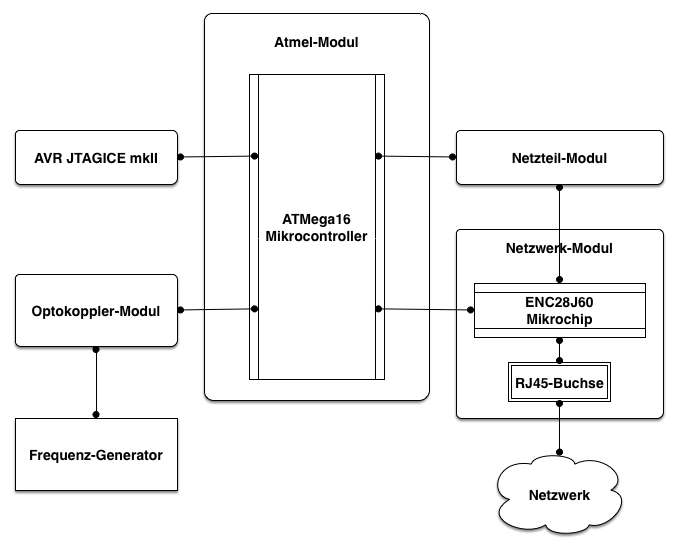
\includegraphics[width=310px,height=250px]{pictures/entwurf.png}
	}
	\caption{Zusammenbau von allen Modulen}\label{fig:aufbau}
\end{figure}

Die \autoref{fig:aufbau} zeigt, wie die einzelnen Module im Gesamtsystem miteinander verbunden sind. Danach wurde der Schaltplan laut dem obigen Gesamtsystem im Eagle\footnote{ist ein Program der Firma CadSoft zur Erstellung von Leiterplatte zur Entwurfsautomatisierung elektronischer Systeme.}-Schaltplaneditor \cite{Cadsoft:Eagle} erstellt. Die Gesamtschaltung ist im \autoref{anhang:schaltung} zu sehen. \smallskip \smallskip

Es wird eine Schnittstelle, sog. \textbf{AVR JTAGICE mkII}, zwischen dem Atmel-Modul und dem verwendeten Rechner angeschlossen. Dieses Modul ermöglicht die Programmierung des ATmega16-Mikrocontrollers. \smallskip \smallskip

Das \textbf{Optokoppler-Modul} liest ein kontinuierlich-sinusförmiges Signal aus dem Frequenzgenerator aus und digitalisiert dieses Signal. Anschließend wird das kontinuerlich-digitalisierte Signal an den Eingangspin des Atmel-Moduls weitergeleitet. \smallskip \smallskip

Das \textbf{Atmel-Modul} liest das Eingangssignal aus dem Pin und sogleich beschäftigt es sich mit der Abarbeitung der Frequenzmessung des Signals mittels eines internen Timers. Nachfolgend werden die Messungswerte dem Netzwerk-Modul abgegeben, wenn sie abgefragt werden. \smallskip \smallskip

Das \textbf{Netzwerk-Modul} ist eine Kommunikationsschnittstelle für das UDP-Protokoll zwischen dem Atmel-Modul und einem beliebigen UNIX-Server. Die Frequenzwerten werden nach Anforderung des Servers über das Netzwerk-Modul weitergegeben. Für die Abfrage wird ein Dämon zum Laufen auf UNIX basierten Systemen programmiert. \smallskip \smallskip

Jedes Modul des Gesamtsystems wird im nächsten Kapitel näher beschrieben. Im \autoref{chapter:protokoll} wurde das Kommunikationsprotokoll näher unter die Lupe genommen. Außerdem ist im \autoref{anhang:software} auch das programmierte Kommunikationsprotokoll zu lesen.


\chapter{Entwurf}\label{chapter:entwurf}

Dieses Kapitel beschäftigt sich mit allen Modulen des Projektes. Unter anderem wird sowohl der Aufbau als auch die Zusammenschaltung mehrerer Module aus der elektrotechnischen Sicht beschrieben, welche in der \autoref{fig:aufbau} grafisch dargestellt wurde.

%%%%%%%%%%%%%%%%%%%%%%%%%%%%%%%%%%%%%%%%%%%%%%%%%%%%%%%%%%%%%%%%%%%%%%%%%%%%%%%
\section{Optokoppler-Modul}

Eine einfache Methode zur Messung der Frequenz eines kontinuierlich-sinusförmigen Signals mit Hilfe eines Mikrocontrollers ist die Digitalisierung dieses Signals, damit die steigenden bzw. fallenden Flanken aufgezählt werden kann. Um dieses sinusförmige Signal zu digitalisieren, wird hier ein \textbf{Optokoppler} benutzt, der ein (Halbleiter-)Bauelement und vor allem in der Nachrichten-Übertragungstechnik sehr nutzbar ist. \smallskip \smallskip

% !!! http://www.renesas.eu/products/opto/technology/ac/index.jsp
Der Optokoppler dient der Signalübertragung zwischen zwei galvanisch vollständig getrennten Stromkreisen in einem gemeinsamen Gehäuse \cite{Mikrocontroller:Optokoppler}. In einem Optokoppler bzw. Gabelkoppler befinden sich ein Lichtsender (\textit{Led}) und ein Lichtempfänger (\textit{Fototransistor}). Die Funktionsweise des Optokopplers ist die Übersetzung von einer sinusförmigen Eingangsspannung zu einer rechteckförmigen Ausgangsspannung \cite{Tietze2002}. Das heißt, dass der Strom am Ausgang über den Fototransistor nur dann fließt, wenn die positive Halbwelle den Lichtsender erreicht. Zusätzlich zu dieser Diode für die positive Halbwelle wird eine Diode für die negative Halbwelle im Eingangsbereich benötigt. In dieser Arbeit findet eine Spannungsquelle im Eingangsbereich mit 10 V (AC) und eine Spannungsquelle im Ausgangsbereich mit 5 V (DC), wie in der \autoref{fig:optokoppler} zu sehen ist.  

\begin{figure}[htbp]
	\centering
	\fbox{
		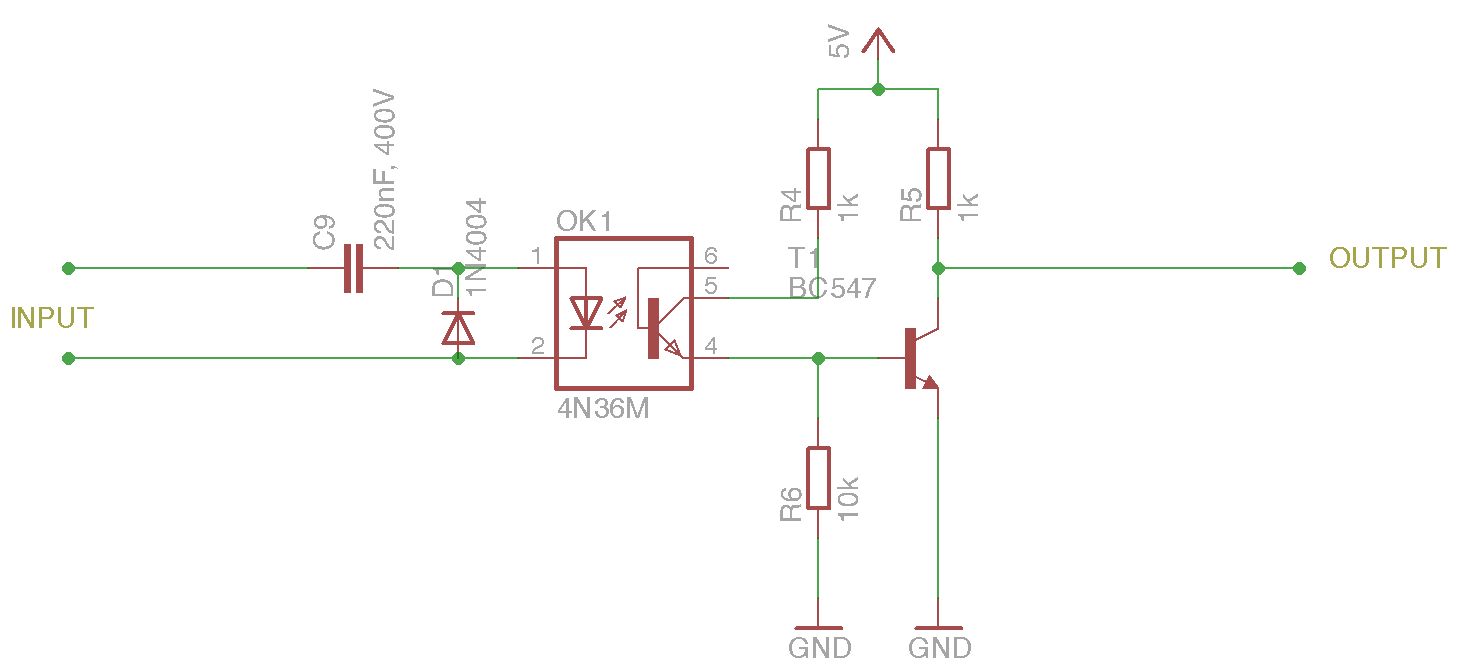
\includegraphics[width=450px,height=203px]{pictures/optokoppler.png}
	}
	\caption{Optokoppler-Modul}\label{fig:optokoppler}
\end{figure}

%%%%%%%%%%%%%%%%%%%%%%%%%%%%%%%%%%%%%%%%%%%%%%%%%%%%%%%%%%%%%%%%%%%%%%%%%%%%%%%
\section{Netzteil-Modul}

Sowohl für das Atmel-Modul als auch für das Netzwerk-Modul wird ein Netzteil benötigt, damit diese an das Netz angeschlossen werden können. Jedes Modul hat eine spezifische Versorgungsspannung. Die Versorgungsspannung beim Atmel-Modul liegt bei $5$ Volt ($\pm 10 \%$) und beim Netzwerk-Modul bei $3.3$ Volt ($\pm 10 \%$). \smallskip \smallskip

Wie in der \autoref{fig:netzteil} zu sehen ist, wird das Atmel-Modul mit $5$ Volt Spannung und das Netzwerk-Modul mit $3.3$ Volt Spannung verbunden.

\begin{figure}[htbp]
	\centering
	\fbox{
		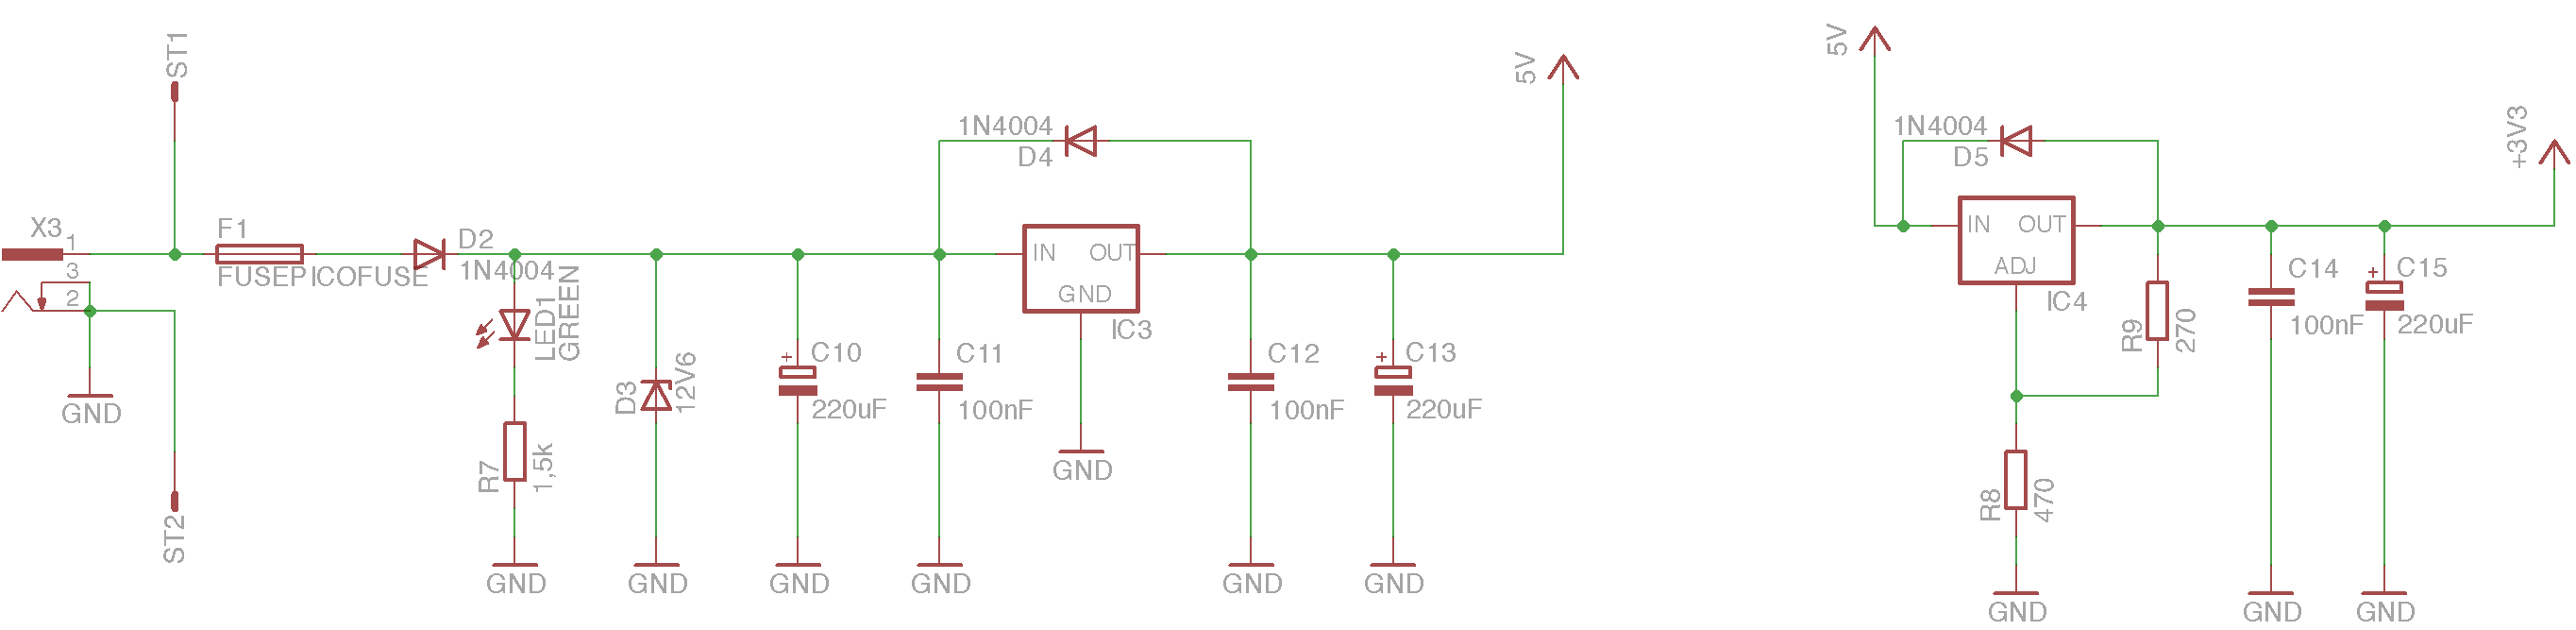
\includegraphics[width=450px,height=110px]{pictures/netzteil.png}
	}
	\caption{Netzteil-Modul}\label{fig:netzteil}
\end{figure}

%%%%%%%%%%%%%%%%%%%%%%%%%%%%%%%%%%%%%%%%%%%%%%%%%%%%%%%%%%%%%%%%%%%%%%%%%%%%%%%
\section{AVR JTAGICE mkII}\label{sec:atmel:jtag}

Um einen funktionierenden Mikrocontroller zu erzielen, muss dieser Mikrocontroller mit einem Entwicklungswerkzeug bzw. mit einem Programmer programmiert werden. Es wurde für diese Arbeit ein Entwicklungswerkzeug vom Firma \textit{ATMEL Corporation} ausgewählt, nämlich \textbf{AVR JTAGICE mkII} \cite{Mikrocontroller:JTAGICEmkII} (siehe \autoref{fig:jtagicemkII}). Dieses Entwicklungswerkzeug bietet die Möglichkeit für das ''On-Chip-Debugging\footnote{On-Chip-Debugging dient die Möglichkeit, mögliche Fehler im Programmcode direkt auf dem Chip zur Laufzeit zu debuggen bzw. zu finden.}'' und die Programmierung über JTAG für alle AVR 8-bit RISC-Mikrocontrollern. Die JTAG-Schnittstelle wurde für ein Test-Access-Port (\textit{TAP}) entwickelt und als \textit{IEEE 1149.1} im Jahr 1990 standardisiert. 

\begin{figure}[htbp]
	\centering
	\fbox{
		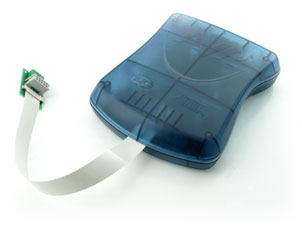
\includegraphics[width=266px,height=200px]{pictures/JTAGICEmkII.jpg}
	}
	\caption[AVR JTAGICE mkII]{AVR JTAGICE mkII \cite{Mikrocontroller:JTAGICE:guide}}\label{fig:jtagicemkII}
\end{figure}

Der JTAGICE-Programmer wird zwischen Entwicklungs- und Zielplattform geschaltet. Er übermittelt somit die Kommunikation zwischen dem Rechner und dem AVR-Mikrocontroller. An den Rechner wird der JTAG-Programmer über ein USB-Kabel angeschlossen und verbraucht keine zusätzliche Versorgungsspannung. An den Mikrocontroller wird der JTAG-Programmer direkt zu den AVR-Pins angeschlossen. Die Pinbelegungen und ihre Beschreibungen sind in der \autoref{fig:jtag}, die Verdrahtung zwischen dem AVR JTAGICE mkII und dem ATMEL-Mikrocontroller in der \autoref{fig:jtag_atmel} beschrieben. 

\begin{table}[htbp]
	\centering
	\begin{tabular}{ |c|c|c|p{9cm}| } \hline
		\textbf{Pin} & \textbf{Signal} & \textbf{I/O} & \textbf{Beschreibung} \\
		\hline
		1 & TCK & Output & Test-Clock, Taktsignal aus JTAGICE mkII zu JTAG-PORT des Ziel-Controllers \\ \hline
		2 & GND & - & Erde \\ \hline
		3 & TDO & Input & Test-Data-Output, Data-Signal aus JTAG-Port des Ziel-Controllers zu JTAGICE mkII \\ \hline
		4 & $V_{ref}$ & Input & Referenzspannung  \\ \hline
		5 & TMS & Output & Auswahl des Testmodes aus JTAGICE mkII zu JTAG-PORT des Ziel-Controllers \\ \hline
		6 & nSRST & OUT-/Input & Zur Steuerung und zur Überwachung über RESET-Pin des Ziel-Controllers\\ \hline
		7 & - & - & nicht verbunden \\ \hline
		8 & nTRST & NC (Output) & nicht verbunden \\ \hline
		9 & TDI & Output &  Test-Data-Input, Data-Signal aus JTAGICE mkII zu JTAG-PORT des Ziel-Controllers \\ \hline
		10 & GND & - & Erde \\ \hline
	\end{tabular}
	\caption{PIN-Belegungen von JTAG-Schnittstelle und ihre Beschreibungen}\label{fig:jtag}
\end{table}

\begin{table}[htbp]
\centering
\begin{tabular}{ |c|c|c|c| }
  \hline
  \multicolumn{2}{|c|}{\textbf{JTAGICE mkII}} & \multicolumn{2}{|c|}{\textbf{ATMega16}}\\ 
  \hline
  TCK & PIN 1& PC2 (PIN 24) & TCK \\
  GND & PIN 2 & GND (PIN 11) & GND \\
  TDO & PIN 3 & PC4 (PIN 26) & TDO \\
  $V_{ref}$ & PIN 4 & VCC (PIN 10) & $V_{ref}$ \\
  TMS & PIN 5 & PC3 (PIN 25) & TMS \\
  nSRST & PIN 6 & RESET (PIN 9) & nSRST \\
  nicht verbunden & PIN 7 & nicht verbunden & nicht verbunden \\
  nTRST & PIN 8 & nicht verbunden & nicht verbunden \\
  TDI & PIN 9 & PC5 (PIN 27) & TDI\\
  GND & PIN 10 & GND (PIN 11) & GND \\
  \hline
\end{tabular}
\caption{Verdrahtung zwischen JTAGICE mkII und ATMega16-Mikrocontroller}\label{fig:jtag_atmel}
\end{table}

%%%%%%%%%%%%%%%%%%%%%%%%%%%%%%%%%%%%%%%%%%%%%%%%%%%%%%%%%%%%%%%%%%%%%%%%%%%%%%%
\section{Atmel-Modul}\label{sec:atmel}

Bei der AVR-Mikrocontroller-Familie von Atmel \cite{Atmel} handelt es sich um 8-Bit Mikrocontroller. Damit die maximale Leistung und die Parallelität erreicht werden kann, verwenden AVR-Mikrocontroller eine Harvard-Architektur\footnote{bezeichnet ein Architekturprinzip zur Realisierung besonders schneller CPUs und Signalprozessoren und erst im Jahr 1959 von \textit{Harvard Mark I} an der Harvard-Universität Cabridge (USA) gestellt.}, in welcher der Befehls- und der Datenspeicher \textit{logisch} und \textit{physisch} von einander getrennt sind (siehe \autoref{fig:avr}). Der Vorteil der Harvard-Architektur liegt darin, dass Befehle und Daten mit einem einzigen Taktzyklus geladen bzw. geschrieben werden. Daher wird diese Architektur in den RISC-Kernen verwendet. Die logische und arithmetische Befehle kommen beim RISC-Kern ein \textit{Dreiadressbefehlsformat}\footnote{Bei Dreiadressbefehlsformat gibt es den Operationscode, die Quelladresse und anschließlich eine Zieladresse.} vor. \smallskip \smallskip

Es wird in dieser Arbeit der AVR-Mikrocontroller-Type \textbf{ATMega16} verwendet, welcher ausreichend genug Leistung für eine einfache Laboranwendung bereitstellt. Der ATMega16-Mikro- controller verfügt über einen 16 KB großen Flashspeicher, in dem die Programme abgelegt werden, und über einen 512 Byte großen EEPROM, das sich in einem separaten Datenbereich befindet, sowie über einen 1 KB großen SRAM-Speicher. Die CPU-Taktfrequenz ist bis zu 16 MHz begrenzt. Es gibt einen 8-Bit bereiten Bus für Daten und einen 16-Bit bereiten Bus für Befehle. Weiterhin bietet der ATMega16 Ein-/Ausgangsschnittstellen, Analog/Digital-Umwandler und 8- bzw. 16-Bit Timers. Zur Kommunikation mit der Außenwelt befinden sich SPI-, U(S)ART-, I$^2$C und JTAG-Schnittstelle. \smallskip \smallskip

Zum Konfigurieren eines AVR-Mikrocontrollers werden \textit{Fuse-Bits} benutzt. Es gibt zwei Bytes (\textit{low} und \textit{high}) zum Konfigurieren von Fuse-Bits. Diese werden beim System-Start des Mikrocontrollers und während dem Betrieb verwendet. Bei einem neuen AVR-Mikrocontroller werden die Fuse-Bits nach der Auslieferung vorkonfiguriert. Die vorkonfigurierten Fuse-Bits werden werksseitig so eingestellt, dass sie den internen RC-Oszillator mit einem 1 $MHZ$ verwenden. Die Fuse-Bits sollen eigentlich nur einmal oder für die notwendigen Anwendungen konfiguriert werden. Die \autoref{tab:fuse-low} und die \autoref{tab:fuse-high} zeigen, welche Aufgaben die jeweiligen Bits von Low- bzw. High-Byte haben. Die Spalte \textit{Konfiguration} zeigt, ob für diese Arbeit die jeweilige Bit programmiert wird oder nicht. Die wichtige Anmerkungen zu den Fuse-Bits sind: 

\begin{itemize}
	\item ''unprogrammiert'' bedeutet, dass der Wert $1$ auf den Fuse-Bit geschrieben ist.
	\item ''programmiert''  bedeutet, dass der Wert $0$ auf den Fuse-Bit geschrieben ist.
\end{itemize}

\begin{table}[htbp]
	\centering
	\begin{tabular}{ |c|c|p{9cm}|c| } \hline
		\textbf{Bit} & \textbf{Fuse Low Byte} & \textbf{Beschreibung} & \textbf{Konfiguration} \\ \hline
		7 & BODLEVEL & Trigger für Brown-Out-Detector\tablefootnote{überwacht die $V_{cc}$ Spannung.}. Wenn der Bit gesetzt ist, ist der minimale Schwellenwert $4.0$ Volt, sonst $2.7$ Volt. & unprogrammiert \\ \hline
		6 & BODEN & Brown-Out Detector aktivieren. Falls BODEN gesetzt ist, wird der AVR-Mikrocontroller mit dem Trigger-Signal neugestartet, wenn $V_{cc}$ unter den Schwellenwert fällt.  & unprogrammiert \\ \hline
		5 & SUT1 & Start-Up-Zeit. Regeln das Bootverhalten des AVR-Mikrocontrollers. & unprogrammiert \\ \hline
		4 & SUT0 & Start-Up-Zeit. Regeln das Bootverhalten des AVR-Mikrocontrollers. & unprogrammiert \\ \hline
		3 & CKSEL3 & Die Taktquelle des Controllers bestimmen. & unprogrammiert \\ \hline
		2 & CKSEL2 & Die Taktquelle des Controllers bestimmen. & unprogrammiert \\ \hline
		1 & CKSEL1 & Die Taktquelle des Controllers bestimmen. & unprogrammiert \\ \hline
		0 & CKSEL0 & Die Taktquelle des Controllers bestimmen. & unprogrammiert \\ \hline
	\end{tabular}
	\caption{Fuse-Bits Low Byte}\label{tab:fuse-low}
\end{table}

\begin{table}[htbp]
	\centering
	\begin{tabular}{ |c|c|p{9cm}|c| } \hline
		\textbf{Bit} & \textbf{Fuse High Byte} & \textbf{Beschreibung} & \textbf{Konfiguration} \\ \hline
		7 & OCDEN & On-Chip-Debugging. Bietet die Möglichekeit ein Echtzeit-Debugging des Mikrocontrollers bei der Aüsführung im Zielsystem. & programmiert \\ \hline
		6 & JTAGEN &  JTAG-Schnittstelle für Debugging. & programmiert \\ \hline
		5 & SPIEN & Serielle Programmierung. & programmiert \\ \hline
		4 & CKOPT & Oszillator-Verstärkung. & programmiert \\ \hline
		3 & EESAVE & Löschen des EEPROM-Speichers beim Programmieren. & unprogrammiert \\ \hline
		2 & BOOTSZ1 & Setzen der Bootloader-Größe. & programmiert \\ \hline
		1 & BOOTSZ0 & Setzen der Bootloader-Größe. & programmiert \\ \hline
		0 & BOOTRST & Falls BOOTRST gesetzt ist, wird das Programm nach dem RESET auf erste Adress des Bootloaders gesprungen. & unprogrammiert \\ \hline
	\end{tabular}
	\caption{Fuse-Bits High Byte}\label{tab:fuse-high}
\end{table}

Die Webseite \textit{engbedded} \cite{Engbedded:Fusecalc} bietet die Möglichkeit auf schnellsten Wege die Konfiguration von Fuse-Bits zu erstellen bzw. zu berechnen. Durch Auswahl des ATMega16-Mikrocontrollers und der benötigten Einstellungen auf der Webseite, gibt sie das High- und das Low-Byte zurück. Für diese Arbeit ist das High-Byte $\mathbf{0x09}$ und das Low-Byte $\mathbf{0xFF}$. Aus diesen zwei Bytes ergibt sich die Spalte ''Konfiguration'' in \autoref{tab:fuse-low} und \autoref{tab:fuse-high}. Nun können die zwei Bytes in den ATMega16-Mikrocontroller geschrieben werden. Um diese Konfiguration zu schreiben, wird das Programm \textit{avrdude} \cite{GNU:Avrdude} mittels der folgenden Kommandozeile im UNIX-Terminal verwendet: %\smallskip \smallskip

%\textbf{\code{avrdude -c PROGRAMMER -P PORT -p PART -U lfuse:w:0xff:m -U hfuse:w:0x09:m\smallskip \smallskip}} 

\begin{minted}[linenos=false, frame=single, fontsize=\scriptsize]{bash}
avrdude -c PROGRAMMER -P PORT -p PART -U lfuse:w:0xff:m -U hfuse:w:0x09:m
\end{minted} 
%\smallskip \smallskip

Für eine ausführliche Erläuterung kann das Benutzerhandbuch \cite{AVRDUDE:Manual} des Programms \textit{avrdude} gelesen werden. \smallskip \smallskip

\begin{figure}[htbp]
	\centering
	\fbox{
		%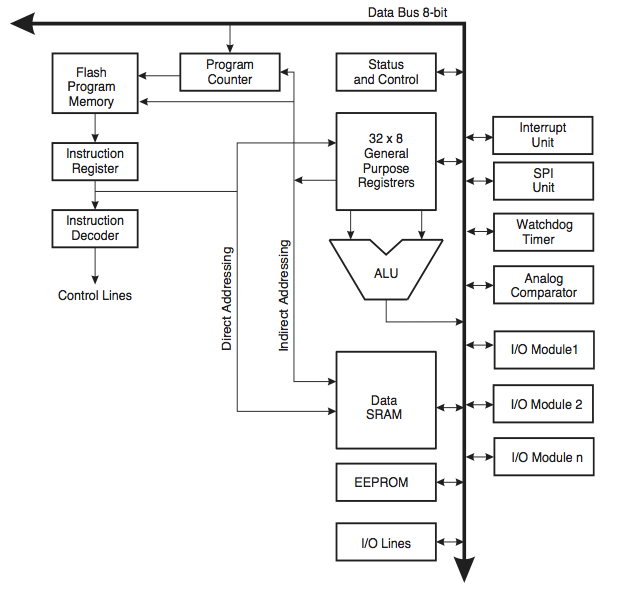
\includegraphics[width=400px,height=385px]{pictures/avr.png}
		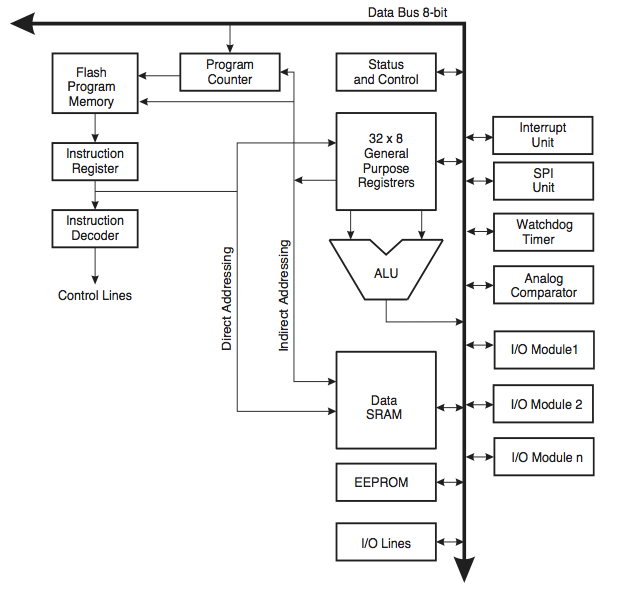
\includegraphics[width=360px,height=355px]{pictures/avr.png}
	}
	\caption[AVR-Architektur]{AVR-Architektur \cite{Atmel:ATMega16}}\label{fig:avr}
\end{figure}

%%%%%%%%%%%%%%%%%%%%%%%%%%%%%%%%%%%%%%%%%%%%%%%%%%%%%%%%%%%%%%%%%%%%%%%%%%%%%%%
\subsection{Timer-Einheit}

Der Timer ist eine Einheit im Mikrocontroller, die einen Zähler enthält und diesen Zähler periodisch inkrementiert und/oder dekrementiert. Unmittelbar nach dem Auftreten eines Ereignisses wird das Hauptprogramm unterbrochen, wobei diese Unterbrechung meist mit dem englischen Begriff \textit{Interrupt} bezeichnet wird. Eine spezielle Art des Interrupts ist das Timer-Interrupt, weil speziell eingestellt werden kann, wann der Interrupt ausgelöst werden soll. Genau genommen ist ein Timer-Interrupt auch ein Zustand\footnote{Wenn der Interrupt auslöst, wird diese Stelle markiert, wobei diese Markierung als \textit{Zeitstempel} in Echtzeit bezeichnet wird.} des Zählers. Grundsätzlich wird der Timer-Interrupt genau dann ausgelöst, wenn der Wert des Zählers einen vordefinierten Wert erreicht oder ein externes Ereignis an einem Pin des Mikrocontrollers auftritt. Der ATMega16-Mikrocontroller hat drei verschiedene unabhängige Timer-Einheiten, wobei zwei mit 8-Bit und ein mit 16-Bit-Auflösung. 

%%%%%%%%%%%%%%%%%%%%%%%%%%%%%%%%%%%%%%%%%%%%%%%%%%%%%%%%%%%%%%%%%%%%%%%%%%%%%%%
\subsubsection{CTC-Modus}

In dieser Arbeit wurde der 16-Bit Timer/Counter1 ausgewählt und dieser wurde im CTC-Modus konfiguriert. In diesem Modus wird der Timer-Interrupt nur dann ausgelöst, wenn der Zähler (\textit{TCNT1}\footnote{Der Timer/Counter\textbf{1}-Zähler ist ein 16-Bit Register und enthält untereinander geschachtelte \textbf{LOW} (\textit{TCNT1L}) und \textbf{HIGH} (\textit{TCNT1H}) Bytes.}) den maximalen Wert (\textit{TOP}) erreicht. Anschließend fängt er wieder bei dem Wert (\textit{BOTTOM}) an (siehe \autoref{fig:timer}). \smallskip \smallskip

\begin{figure}[htbp]
	\centering
	\fbox{
		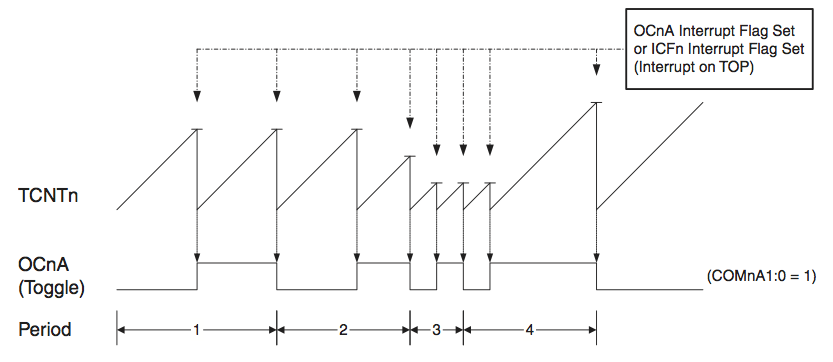
\includegraphics[width=450px,height=195px]{pictures/timer.png}
	}
	\caption[Timer-Diagramm für CTC-Mode]{Timer-Diagramm für CTC-Mode \cite{Atmel:ATMega16}}\label{fig:timer}
\end{figure}
\smallskip \smallskip

%\newpage
Zum Konfigurieren des Timer/Counter1 gibt es zwei Steuerregister, wie in \autoref{tab:tccr1a} und \autoref{tab:tccr1b} beschrieben wird. \smallskip \smallskip

\begin{table}[htbp]
	\centering
	\begin{tabular}{ |c|c|c|c|c|c|c|c|} \hline
		COM1A1 & COM1A0 & COM1B1 & COM1B0 & FOC1A & FOC1B & WGM11 & WGM10 \\ \hline
	\end{tabular}
	\caption{Timer/Counter1 Controler Register A (TCCR1A)}\label{tab:tccr1a}
\end{table}

\begin{table}[htbp]
	\centering
	\begin{tabular}{ |c|c|c|c|c|c|c|c|} \hline
		ICNC1 & ICES1 & (reserviert) & WGM13 & WGM12 & CS12 & CS11 & CS10 \\ \hline
	\end{tabular}
	\caption{Timer/Counter1 Controler Register B (TCCR1B)}\label{tab:tccr1b}
\end{table}

Jedes Bit an den Steuerregistern hat eine spezifische Aufgabe. Änderungen an diesen Bits rufen verschiedene Timer-Modi auf. Bei einem Timer sind verschiedenste Kombinationen möglich, welche im Datenblatt vom ATMega16 zu entnehmen ist. \smallskip \smallskip

Die zwei Byte Steuerregister des Timer/Counter1 sind wie folgt konfiguriert:

\begin{itemize}
	\item CTC-Modus
	\item Der Zähler wurde periodisch in 1 $HZ$ beschränkt.
	\item Input-Capture Noise Canceler
	\item Der Vorteiler wurde mit \textit{256}\footnote{Dies bedeutet, dass der Systemtakt um den Faktor $256$ geteilt wird.} gewählt.
\end{itemize}

%%%%%%%%%%%%%%%%%%%%%%%%%%%%%%%%%%%%%%%%%%%%%%%%%%%%%%%%%%%%%%%%%%%%%%%%%%%%%%%
\subsubsection{Input Capture}

Input Capture ist ein Hardwareteil, der zur genaueren Zeitmessung dient. Das Eingangssignal muss an den ICP angeschlossen werden, um eine Messung durchzuführen. Angewendet wird der Input Capture zwischen zwei aufeinanderfolgende Flanken, wobei die Erkennung entweder auf steigende oder fallende Flanken basiert. \smallskip \smallskip

Der Zähler läuft genau wie im CTC-Modus vom BOTTOM- zum TOP-Wert. Wenn eine eingestellte Zustandsänderung (fallende oder steigende Flanken) am ICP auftritt, wird der aktuelle Zählerwert auf eine Variable übergeben. Bei der nächsten Zustandsänderung wird die Differenz zwischen dem aktuellen Zählerwert und dem zuvor kopierten Zählerwert ermittelt. Diese Differenz ist die Messung zwischen zwei aufeinanderfolgenden Zustandsänderungen. Dieses Szenario findet bei jeder positiven bzw. negativen Flanke fortlaufend statt. 

%%%%%%%%%%%%%%%%%%%%%%%%%%%%%%%%%%%%%%%%%%%%%%%%%%%%%%%%%%%%%%%%%%%%%%%%%%%%%%%
\subsection{SPI-Schnittstelle}
% http://www.uni-koblenz.de/~physik/informatik/MCU/SPI.pdf
% http://www.weigu.lu/a/pdf/MICEL_C4_SPI.pdf
% http://www.netzmafia.de/skripten/hardware/Control/schnittstellen.pdf
% http://wiki.attraktor.org/images/d/d4/Arduino_stammtisch-serielle_kommunikation_spi.pdf
% http://gedankenlyrik.bplaced.net/www/studium/seminararbeit_2008.pdf
% http://avrbeginners.net/architecture/spi/spi.html

Die SPI-Schnittstelle ist ein Bus-System, welches synchron serielle Daten überträgt und von der Firma Motorola entwickelt wurde. Die Funktionsweise basiert auf dem Master-Slave-Prinzip. Die SPI-Schnittstelle unterstützt den richtungsunabhängigen (Full Duplex\footnote{Daten können in beide Richtungen gleichzeitig übertragen werden.}) Nachrichtenaustausch. Die einfache Master-Slave-Verbindung kann wie in der \autoref{fig:spi} hergestellt werden. \smallskip \smallskip

Das Master-Slave-Prinzip ist eine Zugriffsform, bei welcher die höchste Priorität am Bus zu schreiben beim Master liegt. Außerdem entscheidet der Master über den gemeinsam genutzten Übertragungskanal, bei welcher ein oder mehrere Slaves auch angeschlossen sind. Dies führt dazu, dass wenn der Slave den Bus verwenden möchte, muss er warten, dass der Master ihn auffordert, Daten zu senden bzw. zu empfangen. Dieses Prinzip wird sehr oft auch \textit{zentrales Polling}\footnote{Der Master fragt ununterbrochen die Slaves an, ob sie den Bus benötigen.} genannt. \smallskip \smallskip

\begin{figure}[htbp]
	\centering
	\fbox{
		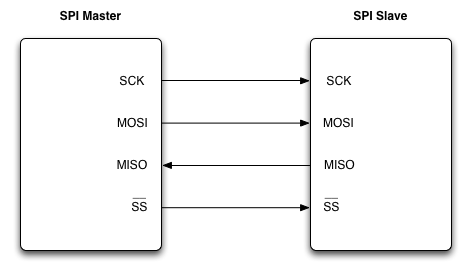
\includegraphics[width=345px,height=200px]{pictures/spi.png}
	}
	\caption{SPI-Verbindung zwichen einem Master und einem Slave}\label{fig:spi}
\end{figure}

Der Übertragungstakt wird vom Master erzeugt und über die Ausgangsleitung (\textit{SCK}-Pin) an alle Slaves geleitet. Im Master-Betrieb muss der SCK-Pin (\textit{PB7}) des ATMega16-Mikrocontrollers als Ausgang eingestellt werden. Im Gegensatz muss der SCK-Pin im Slave-Betrieb als Eingang konfiguriert werden. Dabei wird der $\overline{SS}$-Pin \textbf{LOW} gesetzt, damit der Slave zum Empfangen bereit gestellt wird. Die wichtigste Pins und deren Initialisierungen im Master- und Slave-Betrib werden in der folgenden \autoref{spi:pins} beschrieben: \smallskip \smallskip

\begin{table}[htbp]
	\centering
	\begin{tabular}{ |c|c|c| } \hline
		Pin & Master-Betrieb & Slave-Betrieb \\ \hline \hline
		MOSI & als Ausgang zu initialisieren & automatisch Eingang \\ \hline
		MISO & automatisch Eingang & als Ausgang zu initialisieren \\ \hline
		SCK & als Ausgang zu initialisieren & automatisch Eingang \\ \hline
		$\overline{SS}$ & als Ausgang zu initialisieren & automatisch Eingang \\ \hline
	\end{tabular}
	\caption{Initialisierung von SPI-Pins}\label{spi:pins}
\end{table}

%%%%%%%%%%%%%%%%%%%%%%%%%%%%%%%%%%%%%%%%%%%%%%%%%%%%%%%%%%%%%%%%%%%%%%%%%%%%%%%
\subsection{Debugging}

Bei der Programmierung ist es sehr wichtig zu wissen, in welchem Zustand das Programm sich gerade befindet. Dies erleichtert das Debugging erheblich, da bei jeder Programmabzweigung beispielsweise eine Led eingeschaltet werden kann. Durch das gezielte Ein- bzw. Ausschalten der Leds wird genau erkannt, welchen Pfad das Programm durchläuft. In dieser Arbeit wurde PORTA zum Debugging ausgewählt, an den die Leds verbunden sind. Es können nur so viele Leds als Ausgang dienen, so viele auch als Ausgänge definiert werden. Beispielsweise ist es sehr hilfreich, wenn eine Led für ein bestimmtes Ereignis (z.B. Timer-Interrupt) abwechselnd ein- bzw. ausgeschaltet wird (\textit{toggle}). 

%%%%%%%%%%%%%%%%%%%%%%%%%%%%%%%%%%%%%%%%%%%%%%%%%%%%%%%%%%%%%%%%%%%%%%%%%%%%%%%
\section{Netzwerk-Modul}\label{sec:network}

Damit zwei oder mehrere Geräte miteinander verbunden werden können, um gegenseitig Daten auszutauschen, wird eine Kommunikationsschnittstelle benötigt. Die Kommunikationsschnittstelle baut ein Übertragungskanal zwischen den kommunizierenden Geräten auf. Heutzutage gibt es viele Kommunikationsprotokolle mit verschiedenen Austauschstrategien auf unterschiedlichen Kommunikationsebene. Die Praxis zeigt, dass zwischen den Computern sehr oft das Ethernet-Kanal in Verwendung kommt. Die Vernetzung, welche auf Ethernet-Kanal basiert, wird als LAN bezeichnet. Dieses wird verwendet, um in einem lokalen Netz höhere Datenraten zu erzielen. \smallskip \smallskip

Im nächsten Kapitel werden mehrere Kommunikationsprotokolle näher beschrieben. Dabei wird sowohl der Aufbau als auch die Funktionsweise der einzelnen Schichten der Kommunikationsprotokolle aufgezählt. Auch die hardwarenahe Realisierung des Aufbaus und die Anordnung des Speichermoduls finden in diesem Unterkapitel Platz. 

%%%%%%%%%%%%%%%%%%%%%%%%%%%%%%%%%%%%%%%%%%%%%%%%%%%%%%%%%%%%%%%%%%%%%%%%%%%%%%%
\subsection{Aufbau}
% http://www.rn-wissen.de/index.php/ENC28J60
Der Hersteller \textit{Mikrochip Technology Inc} \cite{Microchip} produziert sehr effiziente Mikrochips für Ethernets. Auch in dieser Arbeit wurde ein Mikrochip dieses Herstellers verwendet, und zwar das Modell \textbf{ENC28J60} \cite{Microchip:ENC28J60}. Dieser Mikrochip ist ein \textit{IEEE 802.3} \cite{IEEE:802.3} kompatibler Ethernet-Controller. \smallskip \smallskip

\begin{figure}[htbp]
	\centering
	\fbox{
		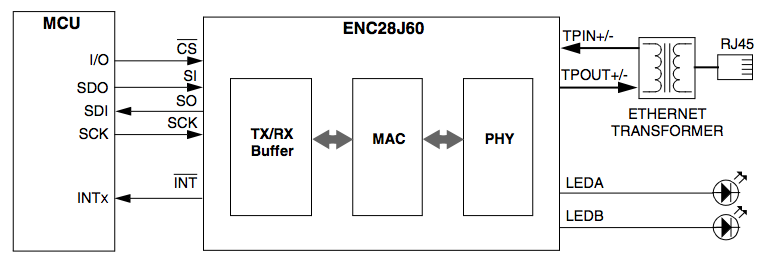
\includegraphics[width=450px,height=155px]{pictures/enc28j60.png}
	}
	\caption[Basisverbindungen zwischen dem ENC28J60 und einem Mikrocontroller]{Basisverbindungen zwischen dem ENC28J60 und einem Mikrocontroller \cite{Microchip:ENC28J60:Datasheet}}\label{fig:enc28j60}
\end{figure}

Der ENC28J60-Mikrochip ist im Gegensatz zu anderen Ethernet-Controllern ein kleiner Chip mit 28-Pins und besitzt einen kleinen Speicher. Es wurde gezielt dieser Mikrochip verwendet, da die Einfachheit und Übersichtlichkeit bei der Laboranwendungen nicht verloren geht. \smallskip \smallskip %Als Nachteil gilt der relativ hohe Stromverbrauch, welche jedoch keine große Relevanz für diese Arbeit hat. \\

Verglichen mit anderen Netzwerk-Mikrochips ist der ENC28J60 klein und dementsprechend auch sehr einfach, ihn in Schaltungen einzubauen. Er enthält eine SPI-Schnittstelle und kann über sie von einem Mikrocontroller leicht angesteuert werden. Die Programmierung der SPI-Schnittstelle ist sowohl im Vollduplex- als auch im Halbduplex-Modus möglich. Allein durch Basisverbindungen des Moduls ist die Funktion gegeben. Wie in der \autoref{fig:enc28j60} zu erkennen ist, handelt sich bei den Basisverbindungen um einige wenige Pins. \smallskip \smallskip

Weiters bietet der ENC28J60 folgende charakteristische Eigenschaften:

\begin{itemize}
	\item integrierten MAC
	\item 10 $MBit/s$ Ethernet-Schnittstelle (10BASE-T Physical Layer)
	\item Voll-/Halb-Dublex Datenverkehr
	\item 8 Kilobytes internen Puffer
	\item SPI-Takt bis zu 25 MHz
\end{itemize}

Um mit einem Rechner im LAN zu kommunizieren, muss der ENC28J60-Mikrochip an eine Ethernet-Buchse angeschlossen werden, wie in der \autoref{fig:enc28j60} dargestellt wurde. Es wird ein festes Kommunikationskabel zwischen dem ENC28J60-Mikrochip und einem Server verlegt. Um das Ethernetkabel an die Buchse anzustecken, wird eine RJ45-Netzwerkstecker benötigt, welcher ein standardisierter Modularstecker ist. Für die \textbf{10BASE-T}-Kommunikation werden nicht alle Adernpaare benötigt. Belegt sind nur zwei Adernpaare, wobei das erste Adernpaar für den Datenausgang und das zweite für den Dateneingang verwendet werden. Diese Adernpaare besitzen je zwei Pins, wobei immer je ein positives und ein negatives Pin für das Eingangs- bzw. Ausgangssignal benötigt werden (siehe \autoref{tab:rj45}). Die Verdrahtung zwischen der RJ45-Buchse und dem ENC28J60-Mikrochip wurde in der \autoref{fig:ethernet} dargestellt. \smallskip \smallskip

\begin{table}[htbp]
	\centering
	\begin{tabular}{ |c|c|c|c| } 
	\hline
		PIN & Signal & Beschreibung & Farbe \\ \hline
		1 & TX+ & positive Sendedaten & weiß/grün \\ \hline
		2 & TX- & negative Sendedaten & grün \\ \hline
		3 & RX+ & positive Empfangsdaten & weiß/orange \\ \hline
		4 & nicht belegt &  & blau \\ \hline
		5 & nicht belegt &  & weiß/blau\\ \hline
		6 & RX- & negative Empfangsdaten & orange \\ \hline
		7 & nicht belegt &  & weiß/orange \\ \hline
		8 & nicht belegt &  & braun \\ \hline
	\end{tabular}
	\caption{Pinbelegung von RJ45-Modularbuchse bzw. -stecker \cite{RJ45:Pins}}\label{tab:rj45}
\end{table}

\begin{table}[htbp]
\centering
\begin{tabular}{ |c|c|c|c| }
  \hline
  \multicolumn{2}{|c|}{\textbf{ENC28J60}} & \multicolumn{2}{|c|}{\textbf{RJ45-Buchse}}\\ 
  \hline
  PIN17 & TPOUT+ & TX+ & 1 \\
  PIN16 & TPOUT- & TX- & 2 \\
  PIN13 & TPIN+ & RX+ & 3 \\
  PIN12 & TPIN- & RX- & 6 \\
  \hline
\end{tabular}
\caption{Verdrahtung zwischen dem RJ45-Buchse und dem ENC28J60-Mikrochip}\label{fig:ethernet}
\end{table}

Wie in der \autoref{fig:enc28j60} zu sehen ist, wird der ENC28J60-Mikrochip nach der Verdrachtung mit dem ATMega16-Mikrocontroller über $\overline{\textbf{CS}}$ ausgewählt werden kann. Die Daten werden über den \textbf{SI}-Pin und über den \textbf{SO}-Pin ein- bzw. ausgelesen, welche mit dem \textbf{SCK} (Takt) von dem Mikrocontroller über die Synchron-Serielle Schnittstelle gesteuert werden können. Mit dem $\overline{\textbf{INT}}$-Pin gibt es eine Möglichkeit zu merken, ob ein passendes Ethernetpaket eingetroffen ist. \smallskip \smallskip

Außerdem besitzt der ENC28J60-Mikrochip zwei Pins (\textit{PIN26} und \textit{PIN27}) für die Leds. Während dem Datenempfang blinkt die \textit{LEDB} und die \textit{LEDA} während der Datensendung. Diese Funktion ist gegeben, wenn die Buchse sie unterstützt. Ansonsten können diese zwei Leds seperat verdrahtet werden, damit das Debugging beim Datenaustausch erleichtert wird. 

%%%%%%%%%%%%%%%%%%%%%%%%%%%%%%%%%%%%%%%%%%%%%%%%%%%%%%%%%%%%%%%%%%%%%%%%%%%%%%%
\subsection{Speicheranordnung}
Der Gesamtspeicher des ENC28J60-Mikrochips wird als statisches RAM implementiert. Der Speicher wurde in drei Teile unterteilt, welche \textbf{Steuerregister}, \textbf{Ethernet-Puffer} und \textbf{PHY-Register} genannt werden, wie in der \autoref{fig:enc28j60_memory} zu sehen ist.  \smallskip \smallskip

\begin{figure}[htbp]
	\centering
	\fbox{
		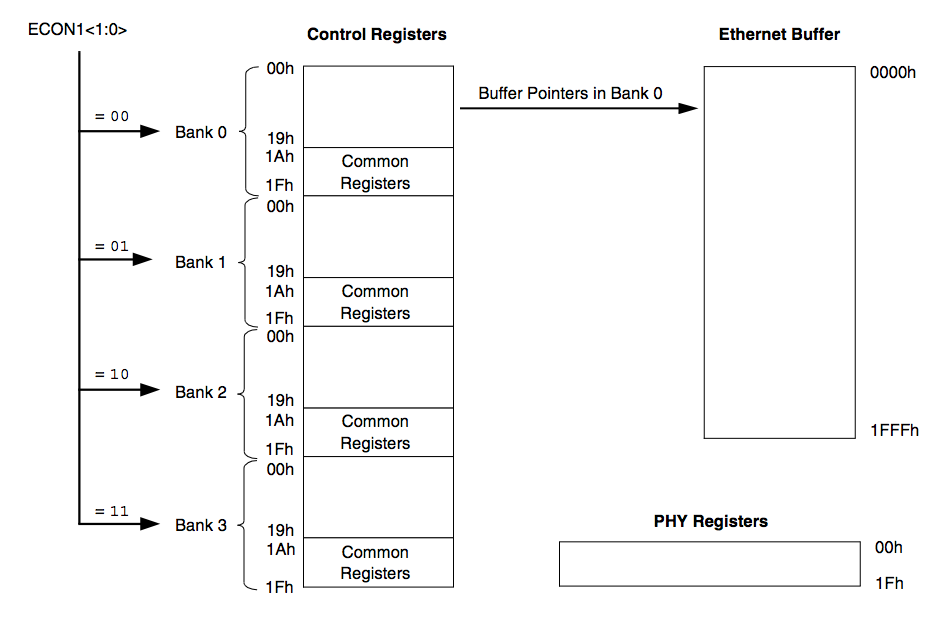
\includegraphics[width=425px,height=280px]{pictures/enc28j60_memory.png}
	}
	\caption[Speicheranordnung des ENC28J60-Mikrochips]{Speicheranordnung des ENC28J60-Mikrochips \cite{Microchip:ENC28J60:Datasheet}}\label{fig:enc28j60_memory}
\end{figure}

Das Steuerungsregister (Control Register) bildet die wichtigste Schnittstelle zwischen dem Mikrocontroller und ENC28J60-Mikrochip. Die Aufgaben des Steuerregisters sind die Konfiguration, die Steuerung und die Überwachung des Mikrochips. Das Steuerregister enthält vier Bänke untereinander. Jede Bank hat eine Größe von 32-Bit. Die letzten fünf Register (von $1B$ bis $1F$) jeder Bank weisen auf die gleichen Registernamen. Sie sind Schlüsselregister, welche als Steuerung bzw. Überwachung des Mikrochips verwendet werden. Um die aktive Bank auszuwählen, wird der \textbf{ECON1<1:0>} (sog. Common Register) eine von vier Kombinationen ($00$, $01$, $10$ oder $11$) für die Bänke gesetzt. \smallskip \smallskip

\begin{figure}[htbp]
	\centering
	\fbox{
		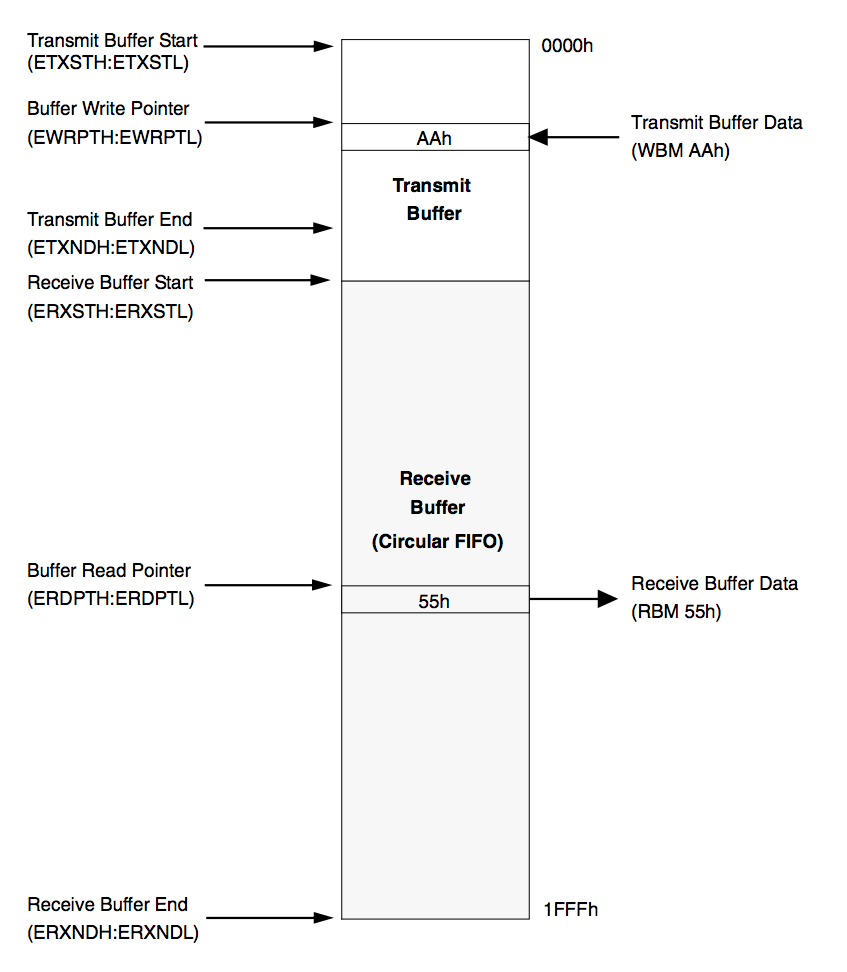
\includegraphics[width=330px,height=380px]{pictures/enc28j60_puffer.png}
	}
	\caption[Pufferanordnung des ENC28J60-Mikrochips]{Pufferanordnung des ENC28J60-Mikrochips \cite{Microchip:ENC28J60:Datasheet}}\label{fig:enc28j60_puffer}
\end{figure}

ENC28J60-Mikrochip hat 8 KB Pufferspeicher. Die erste vier Register der Bank-0 sind Zeiger auf die Adresse des Pufferspeichers, welche zum Lesen und Schreiben gedacht sind. Der Puffer ist unterteilt in zwei, nämlich in Empfangspuffer und Sendepuffer. Die Größe des Sendepuffers ist abhängig von der Größe des Empfangspuffers. Umso größer der Empfangspuffer ist, desto kleiner ist der Sendepuffer. Als Sendepuffer wird dieser Bereich im Speicher bezeichnet, welcher nicht für den Empfang benötigt wird. Die empfangene Daten werden im Empfangspuffer nach dem FIFO-Prinzip (Ringwarteschleife) abarbeitet. Die gesamte Pufferandordung wurde in der \autoref{fig:enc28j60_puffer} dargestellt. \smallskip \smallskip

Um das PHY-Modul zu konfigurieren, wird das \textbf{PHY-Register} verwendet, welches verfügbare 16-Bit beinhaltet. Wegen den Sicherheitsgründen gibt es keinen direkten Zugang über die SPI-Schnittstelle zu diesem Register. Stattdessen wird der Zugang durch einen speziellen Satz von MAC-Steuerregister erzielt.

% http://ww1.microchip.com/downloads/en/AppNotes/00833c.pdf
% http://michaelmoetz.mi.funpic.de/da/datenblaetter/Ethernet_Theory_of_Operation_(Microchip_AN1120)(2008).pdf




\chapter{Ergebnisse}

Zum Abschluss dieser Arbeit wird eine kurze Erklärung von Ergebnissen zusammengefasst. Wie in der \autoref{fig:optocoupler} zu sehen ist, wird ein kontinuierlich-sinusförmiges Signal an den Pin $A$ und Pin $B$ des Optokopplers angeschlossen. Das vom Frequenzgenerator generierte Signal wird in der \autoref{fig:sinus} dargestellt. Die Diode $D1$ spielt hier eine wichtige Rolle, damit der Strom von $B$ nach $A$ fließen kann. Danach wird das Eingangssignal des Optokopplers zwischen den Pin $1$ und Pin $2$ am Oszilloskop gemessen, wie in der \autoref{fig:input} zu sehen ist. Anschließend wird das Eingangssignal mit Hilfe des Optokopplers am Ausgangspin als \textit{digitalisiertes Signal} entnommen, wie in der \autoref{fig:digital} dargestellt wird. \smallskip \smallskip

\begin{figure}[htbp]
	\centering
	\fbox{
		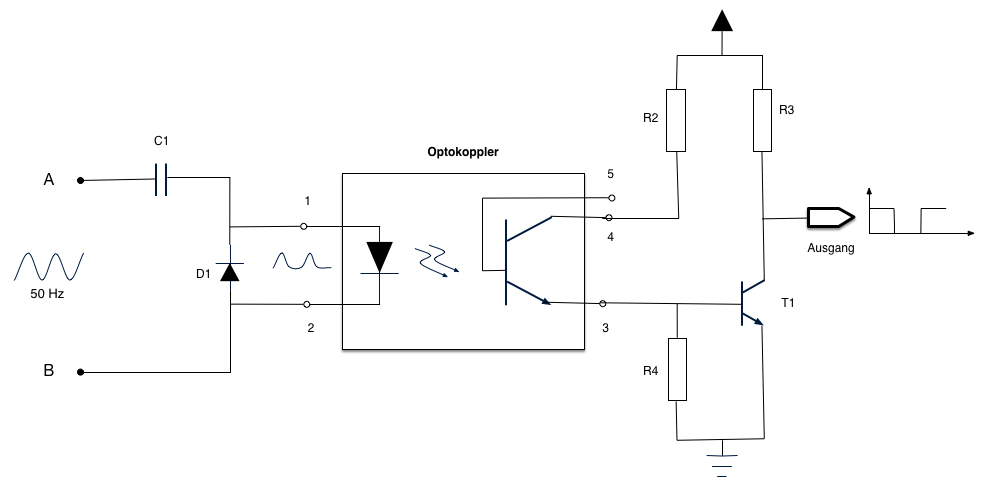
\includegraphics[width=300px,height=160px]{pictures/fazit/optocoupler.png}
	}
	\caption{Schaltplan des Optokopplers}\label{fig:optocoupler}
\end{figure} 

\begin{figure}[ht!]
     \begin{center}
        \subfigure[Sinusförmiges Signal vom Frequenzgenerator]{%
           \label{fig:sinus}
           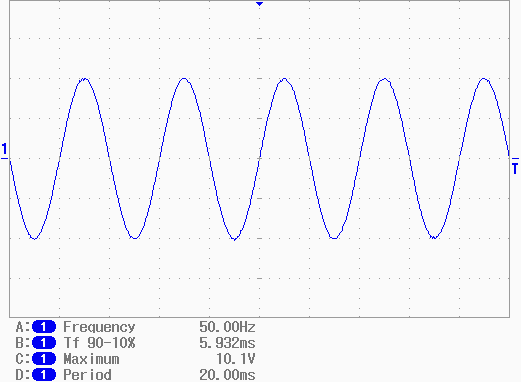
\includegraphics[width=0.45\textwidth]{pictures/fazit/sinus.png}
        }%\\ %  ------- End of the first row ----------------------%
        \subfigure[Eingangssignal des Optokopplers]{%
            \label{fig:input}
            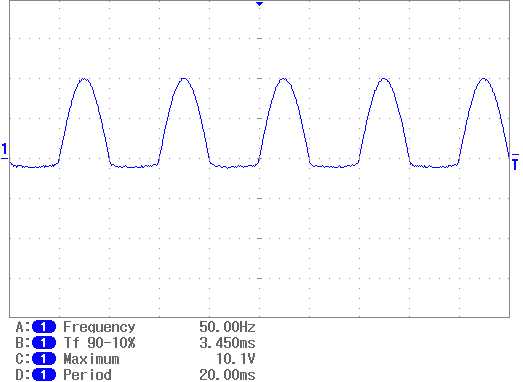
\includegraphics[width=0.45\textwidth]{pictures/fazit/input.png}
        }\\ %
        \subfigure[Digitalisiertes Ausgangssignal des Optokopplers]{%
            \label{fig:digital}
            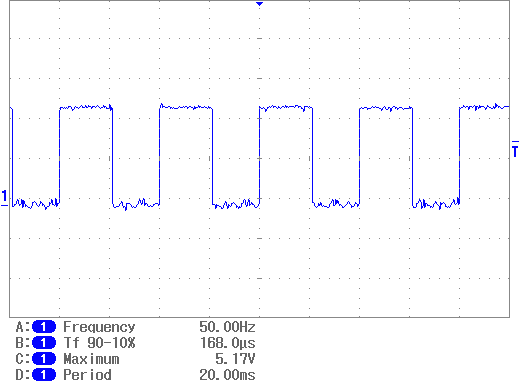
\includegraphics[width=0.45\textwidth]{pictures/fazit/digital.png}
        }%
%
    \end{center}
    \caption{Eingangs- und Ausgangssignale des Optokopplers}%
   \label{fig:signals}
\end{figure}

Am Schluss wird das digitalisierte Signal an den Eingangspin des ATMega16-Mikrocontrollers weitergeleitet. Wenn eine fallende Flanke am Pin des Mikrocontrollers eintrifft, wird der Timer-Interrupt ausgelöst, in dem der Timer-Wert in eine vordefinierte Variable gespeichert wird. Im nächsten Interrupt wird die Differenz zwischen zwei aufeinanderfolgenden fallenden Flanken gespeichert. In der Firmware wird ein Ringpuffer\footnote{ist ein Datenspeicher mit $N$ Datenelementen, wobei der Zeiger ringförmig auf die Datenelemente zeigt.} erstellt, indem die gemessenen Zeitdifferenzen sich befinden. Bei der Abfrage der Frequenz aus dem UNIX-Server werden alle Zeitdifferenzen aus dem Ringpuffer ausgelesen und der Mittelwert berechnet, wie in der folgenden Formel beschrieben wird:

\begin{align}
	Mittelwert = \frac{\sum_{i=1}^{N} Puffer[i]}{N}
\end{align}

wobei $N$ die Länge des Ringpuffers ist. Um die Mittelfrequenz zu berechnen, wird die Taktfrequenz des ATMega16-Mikrocontrollers verwendet, wie in der folgenden Formel beschrieben wird:

\begin{align}
	Mittelfrequenz = \frac{F\_CPU}{Mittelwert * Timer\_Vorteiler}
\end{align}

wobei $F\_CPU$ mit $16$ MHz bestimmt ist, und der $Timer\_Vorteiler$ als $256$ definiert wurde. \smallskip \smallskip 

Nach der Kompilierung der Firmware sieht die Ausgabe folgendemaßen aus:

\begin{minted}[linenos=false, frame=single, fontsize=\scriptsize]{text}
 --- --- --- Target  Information --- --- --- 
      AVR Model       : atmega16
      Board           : Frequenzmessung
      MCU Frequency   : 16000000 Hz
 --- --- --- --- --- --- --- --- --- --- --- 

Size after:
===========================
main.elf  :
section           size      addr
.text             5970         0
.data               12   8388704
.bss               211   8388716
.comment            17         0
.debug_aranges     456         0
.debug_info       9127         0
.debug_abbrev     2740         0
.debug_line       2493         0
.debug_frame      1600         0
.debug_str        1127         0
.debug_loc        5429         0
.debug_ranges       48         0
Total            29230

AVR Memory Usage
----------------
Device: atmega16

Program:    5982 bytes (36.5% Full)
(.text + .data + .bootloader)

Data:        223 bytes (21.8% Full)
(.data + .bss + .noinit)
\end{minted} 

Mit dem \code{ping}-Programm wird eine Abfrage aus dem UNIX-Server an den ENC28J60-Mikrochip gesendet, ob er im Netz verfügbar ist. Es wurde in dieser Arbeit kein DHCP-Protokoll erstellt. Aus diesem Grund muss die IP-Adresse des Mikrochips in der Firmware manual eingetragen werden. Die IP-Adresse ist in der \code{main}-Datei als ''192.168.0.3'' definiert. Wenn der Mikrochip eine richtige IP-Adresse im lokalen Netz besitzt, dann liefert der Mikrochip nach der \code{ping}-Abfrage folgende Antwort zurück: 

\begin{minted}[linenos=false, frame=single, fontsize=\scriptsize]{bash}
$ ping -c 5 192.168.0.3
PING 192.168.0.3 (192.168.0.3): 56 data bytes
64 bytes from 192.168.0.3: icmp_seq=0 ttl=64 time=0.788 ms
64 bytes from 192.168.0.3: icmp_seq=1 ttl=64 time=0.438 ms
64 bytes from 192.168.0.3: icmp_seq=2 ttl=64 time=0.464 ms
64 bytes from 192.168.0.3: icmp_seq=3 ttl=64 time=0.529 ms
64 bytes from 192.168.0.3: icmp_seq=4 ttl=64 time=0.587 ms

--- 192.168.0.3 ping statistics ---
5 packets transmitted, 5 packets received, 0.0% packet loss
round-trip min/avg/max/stddev = 0.438/0.561/0.788/0.125 ms
\end{minted}

Wenn aber der Mikrochip keine gültige lokale IP-Adresse definiert hat, liefert der Mikrochip nach der \code{ping}-Abfrage folgende \textit{Zeitüberschreitungsmeldung}:  \smallskip \smallskip

\begin{minted}[linenos=false, frame=single, fontsize=\scriptsize]{bash}
$ ping -c 5 192.168.0.3
PING 192.168.0.3 (192.168.0.3): 56 data bytes
Request timeout for icmp_seq 0
Request timeout for icmp_seq 1
Request timeout for icmp_seq 2
Request timeout for icmp_seq 3
Request timeout for icmp_seq 4

--- 192.168.0.3 ping statistics ---
5 packets transmitted, 0 packets received, 100.0% packet loss
\end{minted}

Mit dem UNIX-Dämon wird eine Abfrage über das UDP-Protokoll gesendet, um die Mittelfrequenz aus dem ENC28J60-Mikrochip zu erhalten. Der Dämon hat zwei Argumente, IP-Adresse und die Portnummer. Die Argumentbehandlung wird im folgenden Code-Feld beschrieben:  \smallskip \smallskip

\begin{minted}[linenos=false, frame=single, fontsize=\scriptsize]{bash}
$ ./daemon 
Usage: 
	./daemon -h <hostname> -p <port>
	Example: ./daemon -h FreeBSD.local -p 32000
\end{minted}

Wie schon beschrieben wurde, wurde in der Firmware die IP-Adresse ''192.168.0.3'' und die Portnummer ''1200'' definiert. Aus diesem Grund wird der UNIX-Dämon wie in dem folgenden Code-Feld verwendet:

\begin{minted}[linenos=false, frame=single, fontsize=\scriptsize]{bash}
$ ./daemon -h 192.168.0.3 -p 1200
hostname: 192.168.0.3
port number: 1200
sending: start
waiting for packet ...
received packet from 192.168.0.3: 50.153 Hz
\end{minted}

Wie in der letzten Zeile des obigen Code-Felds zu sehen ist, hat der Mikrochip nach der Abfrage die Mittelfrequenz als \textit{50.153 Hz} gesendet bzw. beantwortet.



\chapter{Fazit}

Es werden sowohl elektrotechnische als auch hardwarenahe Kentnisse für diese Arbeit vorausgesetzt. Außerdem werden spezifische Kentnisse über Funktionalität von Computer-Netzwerken benötigt. \smallskip \smallskip

Das Thema war sehr interessant. Nachdem jedoch die unterste Ebene angesprochen wird, wie beispielsweise die TCP/IP-Stacks für die Kommunikationsprotokolle, war die Umsetzung umso komplizierter. Eine große Hilfe bieten die RFC-Dokumente für die Kommunikationsprotokolle. \smallskip \smallskip

Die erste Hürde dieser Arbeit war der Entwurf des Boards, das auf einem Optokoppler, dem ATmega16-Mikrocontroller und auf dem ENC28J60-Mikrochip basiert. Danach wurde das kontinu-ierlich-sinusförmige Signal mit Hilfe des Optokopplers digitalisiert. Um die Frequenzen vom digitalisierten Signal zu messen, wurde der Timer-Treiber im CTC-Modus mit Input-Capture-Betrieb für den Mikrocontroller geschrieben. Der ENC28J60-Mikrochip wurde über die SPI-Schnittstelle angesteuert. Anschließend wurden ARP-, MAC- bzw. TCP/IP-Stacks realisiert. Die Eingangs- bzw. Ausgangssignale wurden schrittweise nach jeder Operation mit dem Osziloskop gemessen. Zur Fehlerbehebung bzw. zum Debuggen wurden Leds verwendet, um zu sehen, ob das Programm bzw. die Firmware auf dem richrigen Pfad läuft. Nach der Abfrage, wie groß der Frequenzwert ist, wurde der mittlere Frequenzwert von letzten zehn Frequentwerte ausgerechnet und als Antwort an den Server übermittelt. \smallskip \smallskip

\chapter{Zukünftige Entwicklung}

Das Projekt ist so umfangreich, dass es mit Zusatzfunktionen ausgestattet werden kann. Beispielsweise könnte ein DHCP-Dienst realisiert werden, sodass der ENC28J60-Mikrochip eine automatische Beziehung der IP-Adresse vom DHCP-Server annimmt, um eine manuelle Eingabe der IP-Adresse zu automatisieren. \smallskip \smallskip

Eine weitere Entwicklung wäre ein NTP-Client. Dieser ermöglicht die Sammlung der Datenpakete von verschiedenen Standorten. Jedes Datenpaket wird mit einem lokalen Zeitstempel versehen. Anhand des Zeitstempels kann der Standort des Datenpakets eruiert werden. Sollten jedoch Datenpakete aus mehreren Standorte in der gleichen Zeitzone ankommen, müssen die Datenpakete mit einer weiteren Kennung gestempelt werden, damit der Server eindeutig identifizieren kann, aus welchem Standort das Datenpaket stammt. Um dieses zu realisieren, müsste jedes Board an verschiedenen Standorten mit einem RTC-Chip ausgestattet sein. \smallskip \smallskip



\makeatletter
\cleardoublepage
\phantomsection

%\chapter{Literaturverzeichnis}
%\addcontentsline{toc}{chapter}{Literatureverzeichnis}

% Publications
\renewcommand\bibname{Literature}
\addcontentsline{toc}{chapter}{Literature}
\label{lite}
\nociteliteratur{*}
\bibliographystyleliteratur{alphadin}
%\bibliographystyleliteratur{plain}
\bibliographyliteratur{bib/literatur}

% Weblinks
\addcontentsline{toc}{chapter}{Weblinks}
\label{web}
\nociteweblink{*}
\bibliographystyleweblink{abbrv}
\bibliographyweblink{bib/weblink}

% Appendix
%\begin{landspace}
%	\begin{multicols}{2}
%		\appendix\label{anhang:a}
%		\chapter{Anhang}
%		\section{Quell-Code}
%		% ---
%	\end{multicols}
%\end{landspace}

\appendix
\begin{landscape}
	\chapter{Anhang}\label{anhang:schaltung}
	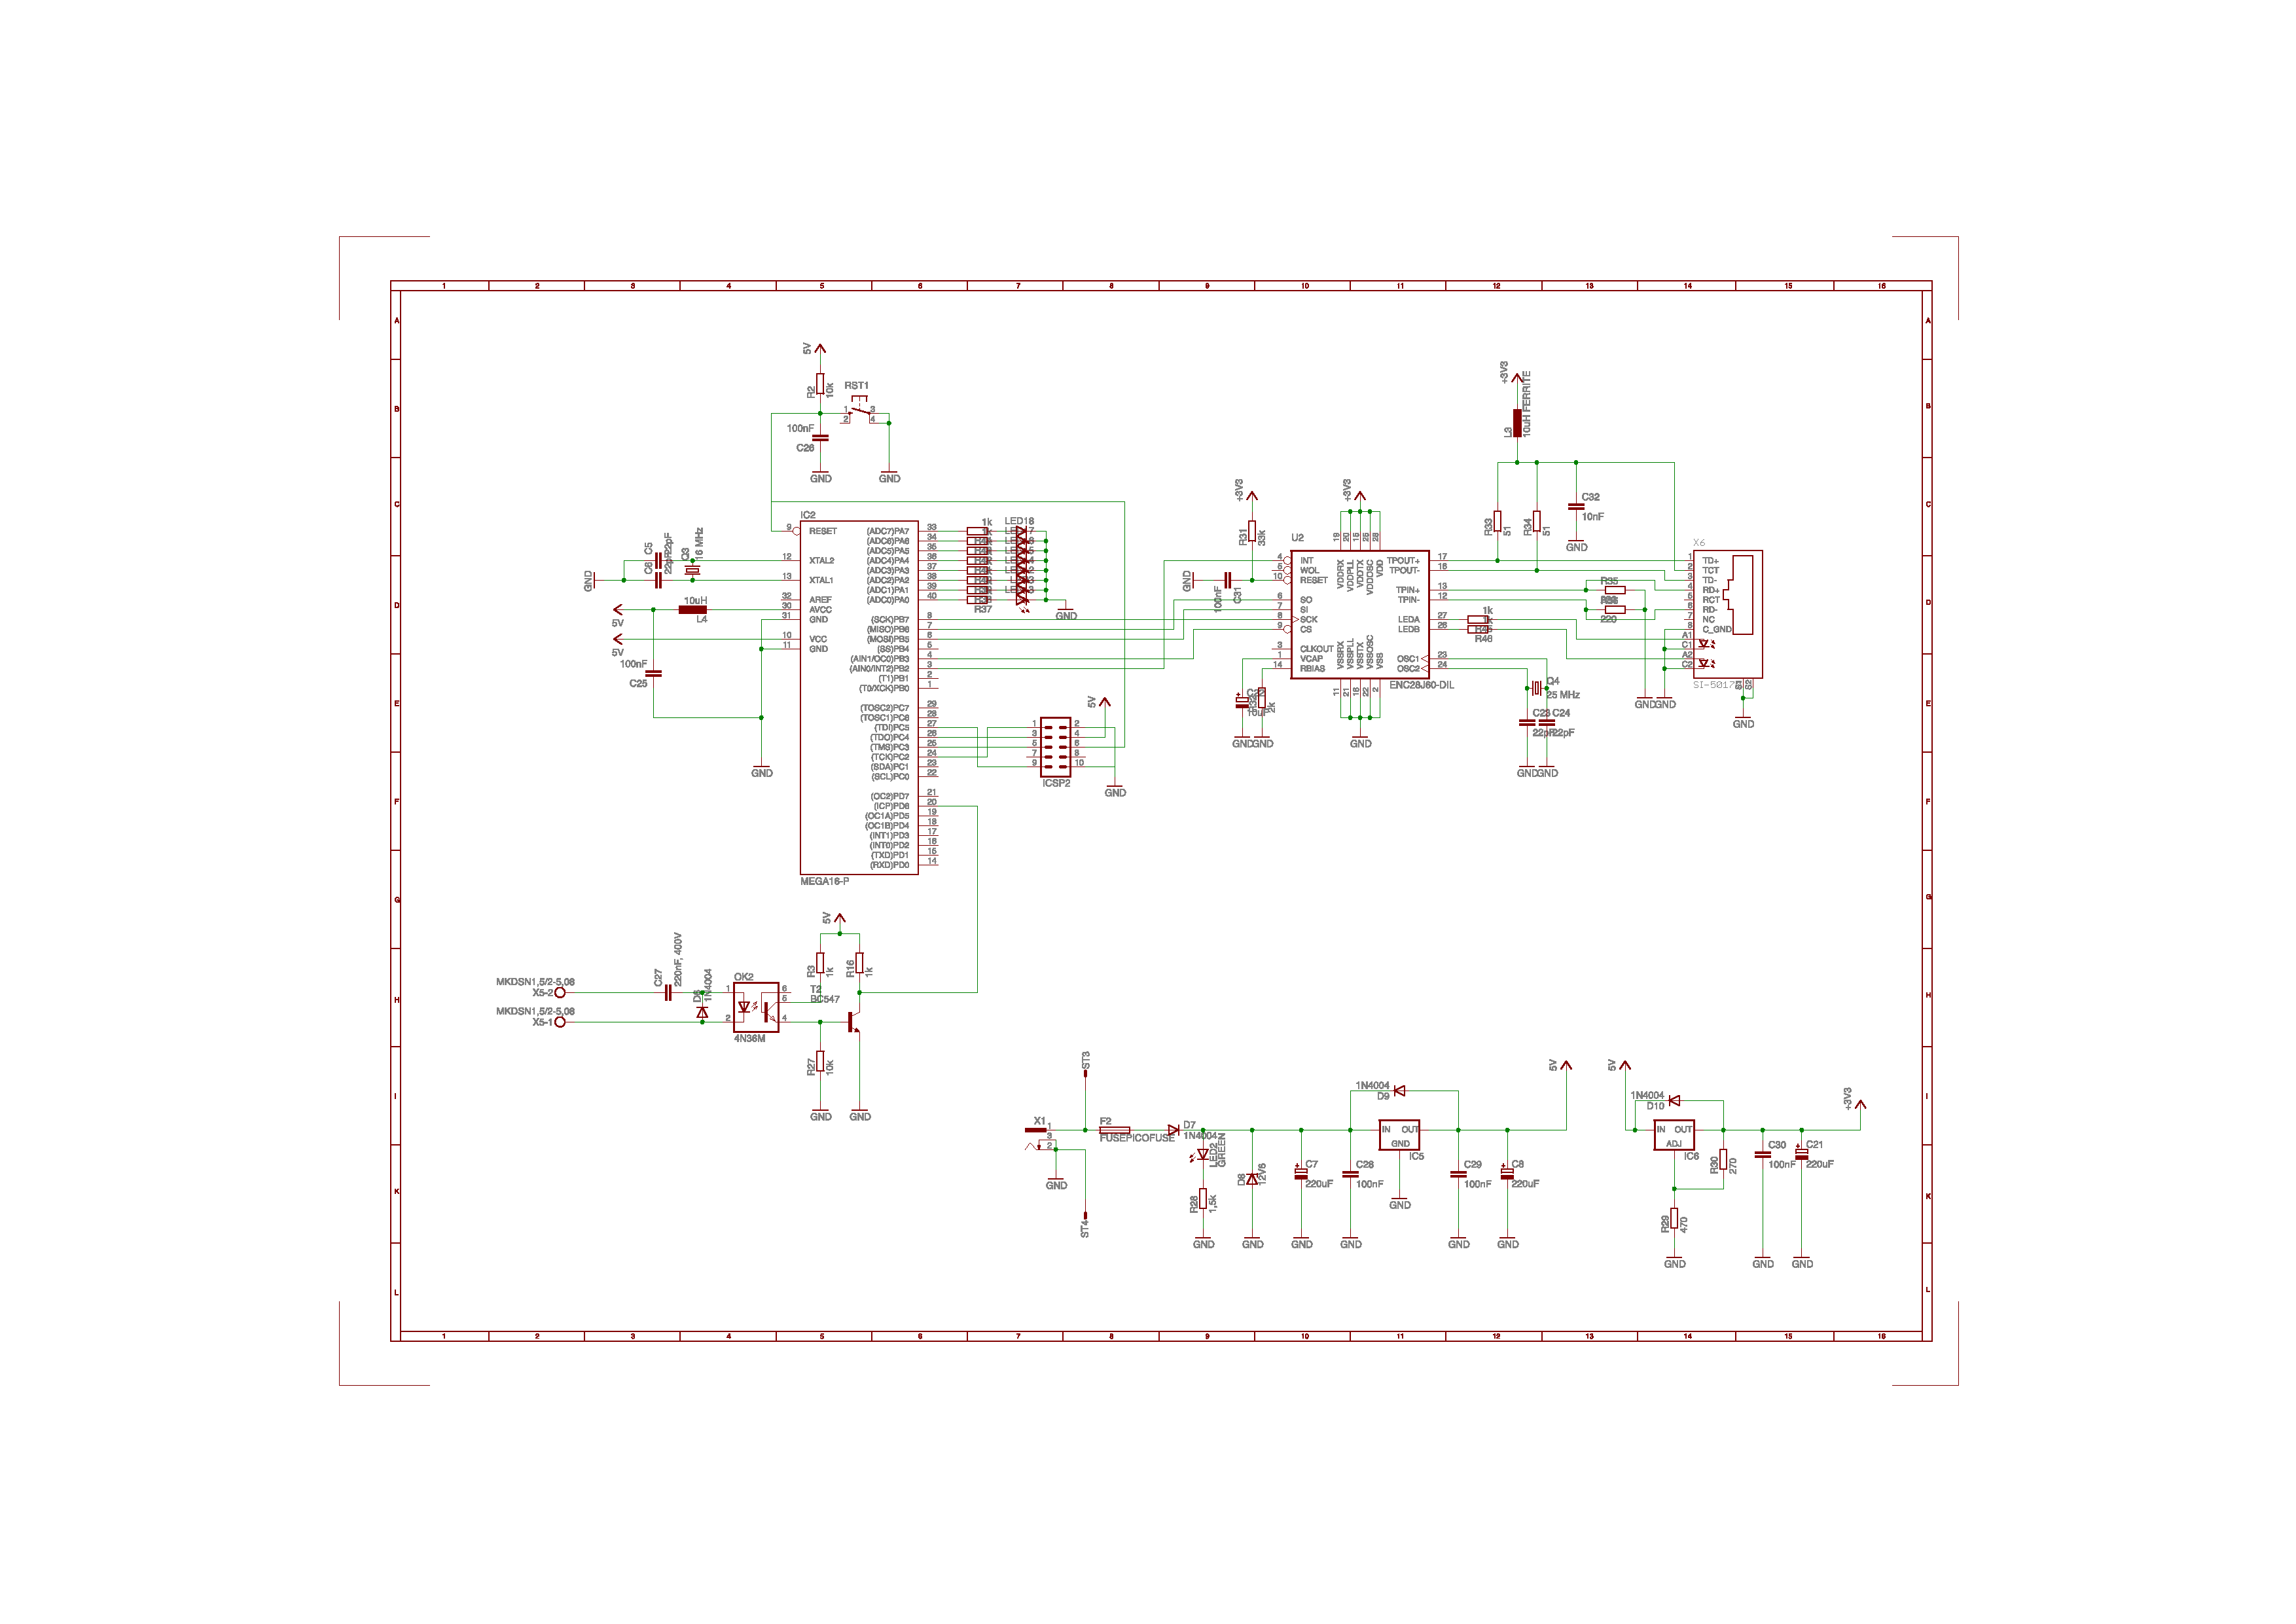
\includepdf[pages=-, landscape]{./pictures/eagle/bachelorarbeit.pdf}
\end{landscape}


%%%%%%%%%%%%%%%%%%%%%%%%%%%%%%%%%%%%%%%%%%%%%%%%%%%%%%%%%%%%%%%%%%%%%%%%%%%%%%%
\begin{landscape}
	\begin{multicols}{2}
		\chapter{Anhang}\label{anhang:software}

		Der Firmware-Code befindet sich in mehreren Verzeichnissen, damit er strukturell noch übersichtlicher ist und die Firmware in Zukunft noch leichter weiter entwickelt werden kann. Unter dem \textit{board}-Verzeichnis befindet sich die Header-Datei, in der die PIN-Belegungen des entworfenen Boards definiert wird. Die Definition des Registers des ATMega16-Mikrocontrollers und des ENC28J60-Mikrochips sind unter dem Verzeichnis \textit{device} zu finden. Die geschriebenen Treiber befinden sich unter dem Verzeichnis \textit{driver}. Um die Zeitmessungswerte zu puffern, gibt es einen \textit{Ringpuffer} im \textit{lib}-Verzeichnis. Schlussendlich stehen die nützliche Definitionen wie \textit{boolean}-Werte und \textit{NULL-Pointer}, falls sie im Compiler nicht definiert ist, im \textit{include}-Verzeichnis zur Verfügung. Die Gesamtstruktur ist in der folgenden Liste zu lesen: \\ \\ \\ \\

		\inputminted[fontsize=\scriptsize]{text}{./code/firmware/README}
		%\input{./code/firmware/firmware}
		\end{multicols}
\end{landscape}

\newpage

\begin{landscape}
Der Firmware-Code und der UNIX-Dämon-Code ist als Open Source Software unter der \textbf{BSD}-Lizenz\footnote{ist eine Lizenz für freie Software. Solche Software darf kostenfrei auch für kommerzielle Zwecke verwendet, verändert und vertrieben werden.} lizenziert bzw. veröffentlicht: \\

\inputminted{text}{./code/LICENSE}
%\input{./code/LICENSE}
\end{landscape}

\newpage

\begin{landscape}
	\begin{multicols}{2}
		\section{Firmware-Code}
		\subsubsection*{main-Programm}
		\subsubsection*{main.c}
		\inputminted[fontsize=\scriptsize,linenos,tabsize=4]{c}{./code/firmware/main.c}

		%%% board %%%
		\subsection*{board-Verzeichnis}
		\subsubsection*{freq.h}
		\inputminted[fontsize=\scriptsize,linenos,tabsize=4]{c}{./code/firmware/board/freq.h}

		%%% device %%%
		\subsection*{device-Verzeichnis}
		\subsubsection*{atmega16.h}
		\inputminted[fontsize=\scriptsize,linenos,tabsize=4]{c}{./code/firmware/device/atmega16.h}

		\subsubsection*{enc28j60.h}
		\inputminted[fontsize=\scriptsize,linenos,tabsize=4]{c}{./code/firmware/device/enc28j60.h}

		%%% driver %%%
		\subsection*{driver-Verzeichnis}
		\subsubsection*{enc28j60.c}
		\inputminted[fontsize=\scriptsize,linenos,tabsize=4]{c}{./code/firmware/driver/enc28j60.c}

		\subsubsection*{icp.h}
		\inputminted[fontsize=\scriptsize,linenos,tabsize=4]{c}{./code/firmware/driver/icp.h}

		\subsubsection*{icp.c}
		\inputminted[fontsize=\scriptsize,linenos,tabsize=4]{c}{./code/firmware/driver/icp.c}

		\subsubsection*{leds.h}
		\inputminted[fontsize=\scriptsize,linenos,tabsize=4]{c}{./code/firmware/driver/leds.h}

		\subsubsection*{leds.c}
		\inputminted[fontsize=\scriptsize,linenos,tabsize=4]{c}{./code/firmware/driver/leds.c}

		\subsubsection*{net.h}
		\inputminted[fontsize=\scriptsize,linenos,tabsize=4]{c}{./code/firmware/driver/net.h}

		\subsubsection*{net.c}
		\inputminted[fontsize=\scriptsize,linenos,tabsize=4]{c}{./code/firmware/driver/net.c}

		\subsubsection*{spi.h}
		\inputminted[fontsize=\scriptsize,linenos,tabsize=4]{c}{./code/firmware/driver/spi.h}

		\subsubsection*{spi.c}
		\inputminted[fontsize=\scriptsize,linenos,tabsize=4]{c}{./code/firmware/driver/spi.c}

		\subsubsection*{timer0.h}
		\inputminted[fontsize=\scriptsize,linenos,tabsize=4]{c}{./code/firmware/driver/timer0.h}

		\subsubsection*{timer0.c}
		\inputminted[fontsize=\scriptsize,linenos,tabsize=4]{c}{./code/firmware/driver/timer0.c}

		%%% include %%%
		\subsection*{include-Verzeichnis}
		\subsubsection*{common.h}
		\inputminted[fontsize=\scriptsize,linenos,tabsize=4]{c}{./code/firmware/include/common.h}

		\subsubsection*{stdbool.h}
		\inputminted[fontsize=\scriptsize,linenos,tabsize=4]{c}{./code/firmware/include/stdbool.h}

		%%% lib %%%
		\subsection*{lib-Verzeichnis}
		\subsubsection*{buffer.h}
		\inputminted[fontsize=\scriptsize,linenos,tabsize=4]{c}{./code/firmware/lib/buffer.h}

		\subsubsection*{buffer.c}
		\inputminted[fontsize=\scriptsize,linenos,tabsize=4]{c}{./code/firmware/lib/buffer.c}

		%%% Makefile %%%
		\subsection*{Makefile(s)}
		\subsubsection*{BSDmakefile}
		\inputminted[fontsize=\scriptsize,linenos,tabsize=4]{c}{./code/firmware/BSDmakefile}

		\subsubsection*{GNUmakefile}
		\inputminted[fontsize=\scriptsize,linenos,tabsize=4]{c}{./code/firmware/GNUmakefile}

		\subsubsection*{config.mk}
		\inputminted[fontsize=\scriptsize,linenos,tabsize=4]{c}{./code/firmware/config.mk}

		\subsubsection*{Makefile.mk}
		\inputminted[fontsize=\scriptsize,linenos,tabsize=4]{c}{./code/firmware/Makefile.mk}

		\subsubsection*{Makefile}
		\inputminted[fontsize=\scriptsize,linenos,tabsize=4]{c}{./code/firmware/Makefile}

		\newpage
		
		%%% UNIX daemon %%%
		\section{UNIX-Dämon}
		\subsection*{main-Programm}
		\subsubsection*{main.c}
		\inputminted[fontsize=\scriptsize,linenos,tabsize=4]{c}{./code/daemon/src/main.c}

		\subsection*{UDP-Protokoll}
		\subsubsection*{udp.h}
		\inputminted[fontsize=\scriptsize,linenos,tabsize=4]{c}{./code/daemon/src/udp.h}

		\subsubsection*{udp.c}
		\inputminted[fontsize=\scriptsize,linenos,tabsize=4]{c}{./code/daemon/src/udp.c}

		\subsection*{Fehlerbehandlung}
		\subsubsection*{error.h}
		\inputminted[fontsize=\scriptsize,linenos,tabsize=4]{c}{./code/daemon/src/error.h}

		\subsubsection*{error.c}
		\inputminted[fontsize=\scriptsize,linenos,tabsize=4]{c}{./code/daemon/src/error.c}

		%%% Makefile ??? %%%
		
	\end{multicols}
\end{landscape}


\end{document}